\documentclass{revista}

\Numero{002}
\Data{Maio 2025}
%\ImaxePortada{revistas/002/imaxes/portada.jpeg}
\ImaxePortada{portadadurisima.jpeg}
\ComentarioImaxePortada{ Sinal dunha maratón en Taiwán. Reza: ``Non fai falla apurarse, hai moito tempo para traballar nunha solución. }
\CorResalte{0000ff}
\CorTextoEnResalte{ffffff}
%\CorResalte{ff2ce8}
%\CorTextoEnResalte{ffffff}
%\SobreMomentum{ Estamos de volta co novo número da revista estudantil momentum, unha revista que busca ser un medio de comunicación tanto dentro coma fóra da facultade de física onde expor os intereses científicos do estudantado. Cuestións de Divulgación, Actualidade, Entrevistas, Historia, Filosofía da Ciencia, Opinión, Programación... Son todos temas que teñen cabida dentro deste proxecto. Esta revista está realizada integramente polo estudantado da Facultade de Física USC, onde pretendemos ter un recuncho de expresión máis aló do estrictamente académico. Fundada no ano 2025 co obxectivo de persistir na historia, esforzámonos sempre en mellorar. Non dubidedes en deixar a vosa pegada!
% }
\Participantes{%
    {\Large \textbf{Dirección}}      \\[0.5cm] %
        Álvaro Pallas Otero          \\[0.2cm] %
        Sebastián Táboas Pazo        \\[0.2cm]% 
        Celia Álvarez Álvarez        \\[0.2cm]%
        Daniel Vázquez Lago          \\[0.75cm]%
    {\Large \textbf{Edición e Corrección}}        \\[0.5cm]%
        David Cotelo Varela          \\[0.2cm] %
        Andrea Real Blanco           \\[0.2cm] %
        Víctor Díaz Díaz             \\[0.2cm] %
        Cristóbal Santos Sánchez     \\[0.2cm] %
        Hugo Raíndo Lorenzo          \\[0.75cm] %
    {\Large \textbf{Deseño de Logo}} \\[0.5cm]%
        Ana Díaz Caride              \\[0.2cm] %
        Elena López Miguélez         \\[0.2cm] %
}
\Despedida{%
Aquí está a revista por e para estudantes da Facultade de Física USC! Cansos de que o momento lineal e angular guíen as nosas traxectorias?, imos escribir unha nova historia; entrevistas, divulgación, filosofía da ciencia e moitos artigos dispares cargamos coa inercia de formar unha nova fiestra para o alumnado. Tes nas túas mans esta oportunidade, deixa que o magnetismo te leve e participa, sé parte deste proxecto: escribe, le, comparte, suxestiona… A revista é real e as túas ideas poden ser máis que imaxinación, non dubides en deixar a túa pegada neste recuncho físico, onde hai física máis aló \centerline{das aulas.}}

\Agradecementos{%
Dende a dirección da revista, queriamos agradecervos a todos por achegarvos a este proxecto. Non hai revista sen lector! Mais, para facela, estivo moita xente implicada que non podemos pasar por alto.\\[0.25cm]
Grazas a todas esas persoas que recibiron acaloradamente a nosa primeira entrega e axudounos a mellorar coas súas suxestións. Especiais grazas ao alumnado que se esmereou na corrección e edición deste número en medio da recta final do cuatrimestre.\\[0.25cm]
Grazas a Ana Ulla, por participar nesta nova entrega dun proxecto que está apenas comenzando, e a Gemma Ruíz, por permitirnos coñecer a esta compañeira tan espectacular.\\[0.25cm]
Grazas a Carlos Merino por participar con toda a súa bondade esta vez escribindo un artigo e trasmitíndonos toda a súa ilusión polo proxecto.\\[0.25cm]
E grazas finalmente tanto ao equipo decanal da nosa facultade como á vicerreitoría de estudantes e cultura polo seu apoio e colaboración neste proxecto, cubrindo ademais esta última a financiación da edición impresa.}

\begin{document}
\pagenumbering{gobble}
\thispagestyle{empty}

% Creamos unha xeometria nova
\newgeometry{
    top    = 2mm,  % marxe superior
    left   = 5mm,  % marxe esquerdo
    right  = 5mm,  % marxe dereito
    bottom = 5mm,  % marxe inferior
    nohead = true, % desactivar o encabezado
    nofoot = true, % desactivar o pe de paxina
}

\begingroup % un grupo para que o de parindent non afecte ao resto da revista
\setlength\parindent{0pt}

% TITULO %%%%%%%%%%%%%%%%%%%%%%%%%%%%%%%%%%%%%%%%%%%%%%%%%%%%%%%%%%%%%%%%%%%%%
\vspace*{3mm}
{%
    \centering%
    \fontsize{70pt}{0pt}\selectfont%
    \FormateaTitulo{Resalte}\par%
}%
\vspace*{6mm}
{%
    \centering%
    \fontsize{18pt}{0pt}\selectfont%
    \textsf{A revista estudantil da Facultade de Física da USC}\par%
}%
\vspace*{7mm}

% NUMERO DA REVISTA E DATA %%%%%%%%%%%%%%%%%%%%%%%%%%%%%%%%%%%%%%%%%%%%%%%%%%%
{
\setstretch{0}
\begin{tcolorbox}[
    colback  = Resalte,
    colframe = black,
    boxrule  = 2pt,
    boxsep   = 6pt,
    sharp corners,
]%
    {
        \fontsize{20pt}{0pt}\selectfont%
        \color{TextoEnResalte}\texttt{\imprimeNumero\hfill\imprimeData}\par%
    }%
\end{tcolorbox}
}

% IMAXE DE CADA REVISTA %%%%%%%%%%%%%%%%%%%%%%%%%%%%%%%%%%%%%%%%%%%%%%%%%%%%%%
% A imaxe da portada debe ser CADRADA EXACTAMENTE
{
\vspace*{-4pt}
\nointerlineskip
\begin{picture}(\textwidth,\textwidth)%
    \put(0,0){%
        \setlength{\fboxsep}{0pt}%
        \setlength{\fboxrule}{2pt}%
        \fbox{%
            \includegraphics[width=\textwidth-4pt]{\imprimeImaxePortada}%
        }%
    }%
\end{picture}
}

% IMAXES SUPERPOSTAS NA IMAXE DA PORTADA %%%%%%%%%%%%%%%%%%%%%%%%%%%%%%%%%%%%%
\begin{tikzpicture}[remember picture, overlay]
    % Imagen 1 (superpuesta)
    \node[
        anchor       = south west,
        xshift       = 0.9cm,
        yshift       = 3.7cm,
        fill         = gray,
        fill opacity = 0.75, % transparencia del fondo
        text opacity = 1,    % el texto sigue opaco
        % draw,              % opcional, para dibujar el borde
        % rounded corners,   % opcional, para esquinas redondeadas
        inner sep=5pt        % separación interna del texto al borde
    ]  at (current page.south west)
    {\normalsize \textcolor{white}{\imprimeComentarioImaxePortada} };

    % Imagen 2 (superpuesta)
    \node[
        anchor = south west,
        xshift = 0.55cm,
        yshift = 0.5cm
    ] at (current page.south west)
    {
\includegraphics[width=12cm]{logos/vicerreitoria-branco-negro.pdf}};
\end{tikzpicture}
\endgroup% <-- este cerra o grupo que contén o de \setlenght\parindent{0pt}

% volvemos a cargar a xeometria que tiñamos no preambulo
\restoregeometry

\begingroup % un grupo para que o de parindent non afecte ao resto da revista
\setlength\parindent{0pt}
% Color del resalte trasparentado a la derecha del índice
\begin{tikzpicture}[remember picture, overlay]
    \draw[
        line width = 0.73\textwidth,
        color      = Resalte!65!white
    ] ($(current page.north east) - (0,0)$) -- ($(current page.south east) - (0,0)$);
\end{tikzpicture}
% (non xoguedes a poñer liñas en blanco entre as tikzpictures, vai ir mal)
%
% %%%%%%%%%%%%%%%%%%%%%%%%%%%%%%%%%%%%%%%%%%%%%%%%%%%%%%%%%%%%%%%%%%%%%%%%%%%%
% Columna de la izqueirda, está el índice y el Sobre Momentum. Para colocar ben
% as as cousas hai que usar moitos 'minipage'.
\begin{minipage}[t]{0.72\textwidth}%
    \vspace{-0.3cm}%
    \begin{minipage}[t]{\hsize}%
        \makebox[0pt][l]{%
            % :FACER: se metemos moitas cousas, non colle
            %
            % ============ TOC ===============================================
            % Aquí incluimos el tableofcontens. Personalizado aparte no arquivo
            % 'revista.cls', botádelle un ollo ao comando \SeccionTOC
            \begin{adjustbox}{valign=t,minipage={0.9\textwidth},margin={0pt,0pt}}
                {
                    \section*{\Huge \textbf{Índice}}
                    \begingroup%
                        % Esto es para que no salte el Indice default, y lo
                        % podamos poner nosotros
                        \let\contentsname\relax%
                        \tableofcontents% <--- o 'TOC' CARGASE AQUí
                    \endgroup%
                }%
            \end{adjustbox}%
        }%
        % ============== SOBRE MOMENTUM =======================
        % Texto debajo del índice, sobre momentum
        \vfill
        \begin{minipage}[t]{0.9\textwidth}
            \vfill
            \vspace{2cm}
            %{\Huge \color{Resalte!75!black} \textbf{Sobre Momentum}:} \\[1cm]
            %\imprimeSobreMomentum
        \end{minipage}
    \end{minipage}
\end{minipage}
\hfill
%
% %%%%%%%%%%%%%%%%%%%%%%%%%%%%%%%%%%%%%%%%%%%%%%%%%%%%%%%%%%%%%%%%%%%%%%%%%%%%
% %%%%%%%%%%%%%%%%%%%%%%%%%%%%%%%%%%%%%%%%%%%%%%%%%%%%%%%%%%%%%%%%%%%%%%%%%%%%
% LADO DEREITO COS PARTICIPANTES, VARIOS LINKS, DATA, etc. Resaltado cunha cor
%
\begin{minipage}[t]{0.28\textwidth}
    \vspace{-0.3cm}
    \hspace{-0.7cm}
    % Data e Número da revista
    \begin{center}
        \textcolor{TextoEnResalte}{\Large
            \textbf{\today }\\[5mm]
            \textbf{\imprimeNumero} \\[1.5cm]
        }
    \end{center}
    % Aquí mostramos as persoas que participaron no proxecto.
    \imprimeParticipantes \\[1.5cm]
    % Links varios
    \begin{tikzpicture}[scale=1.5]
        \begingroup
        \hypersetup{urlcolor = TextoEnResalte}
        \node at (0,0) { \FonteSimbolos\fontsize{20pt}{0pt}\selectfont \textcolor{TextoEnResalte}  };
        \node[
            anchor = west,
            align  = left
        ] at (0.3,0)
        {
            \footnotesize \href{mailto:\imprimeCorreo}{\textbf{\imprimeCorreo}}
        };
        % \node at (0,-1) {\FonteSimbolos\fontsize{20pt}{0pt}\selectfont \textcolor{TextoEnResalte}  };
        % \node[
        %     anchor = west,
        %     align  = left
        % ] at (0.5,-1)
        % {
        %     \href{https://github.com/\imprimeLinkRepositorio}{\texttt{\imprimeLinkRepositorio}}
        % };
        \endgroup
    \end{tikzpicture} \\[1.7cm]
    %
    % Logo da USC
    \begin{center}
        
\includegraphics[width=0.8\linewidth]{logos/usc-negativo-escuro.pdf}
    \end{center}
\end{minipage}
\endgroup % <-- este cerra o grupo que contén o de \setlenght\parindent{0pt}
\newpage
\pagenumbering{arabic}


\Titular*%
{Coñecendo a Ana Ulla Miguel}%
{Gemma Ruíz Lavandeira}%
{entrevistas}%
{Camiños na astrofísica, desafíos e horizontes futuros.}%
%Conversa de tal coa astrofísica Ana Ulla Miguel.}%

\begin{refsection}
\begin{multicols}{2}

\subsection*{Biografía}
Ana Ulla Miguel comezou a licenciatura en Ciencias Físicas na Universidade de
Santiago de Compostela, para logo especializarse en astrofísica na Universidad
de La Laguna, lugar onde obtería o seu título de doutora en 1993. Entre 1988 e
1995, ocupou diversos postos de investigación e docencia na Universidade de
Tromsø (Noruega), o Laboratorio de Astrofísica Espacial e Física Fundamental
(Madrid), a \textit{Axencia Espacial Europea} (ESA) ou o Instituto Niels Bohr
(Copenhague). Posteriormente, foi contratada posdoutoral no Instituto de
Astrofísica de Canarias (IAC), traballando no proxecto ``\textit{Infrared
Space Observatory}'' (ISO) da ESA.

\begin{center}
    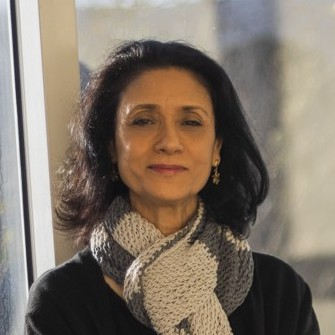
\includegraphics[width=0.85\linewidth]{revistas/002/imaxes/PHOTO-2025-04-30-18-18-48.jpg}
    \captionof{figure}{Ana Ulla Miguel, astrofísica e catedrática na Universidade de Vigo.}
\end{center}

Dende 1997 é docente do Departamento de Física Aplicada da Universidade de
Vigo, sendo a investigadora principal do Grupo AS1 de Astronomía e Astrofísica
da UVIGO dende a súa creación no ano 2005 ata outubro de 2017. Dende 2022 é
catedrática de astronomía e astrofísica do mesmo departamento e investigadora
do grupo GEOMA (\textit{Xeoloxía Mariña e Ambiental}) integrado no CIM
(\textit{Centro de Investigación Mariña}) da UVIGO. Os seus intereses de
investigación inclúen, entre outros temas, a evolución estelar en fases avanzadas, os exoplanetas ou a astrobioloxía. Forma parte do grupo galego da misión Gaia, da ESA, xunto con outros compañeiros da Universidade da Coruña (UDC) e a Universidade de Cantabria (UNICAN).

\subsection*{Entrevista}

\paragraph{Gemma:} En primeiro lugar, Ana, moitas grazas por participar na nosa
revista e acceder a contestar unhas preguntas para coñecer máis sobre ti e
sobre o teu traballo. É un grande orgullo poder contar co teu testemuño. Para
comezar, poderías contarnos como xurdiu o teu interese por estudar Física e
posteriormente Astrofísica?

\paragraph{Ana:} Grazas a vós por convidarme para esta entrevista e parabéns pola
iniciativa da vosa revista.

Dende a adolescencia souben que quería entender o mundo e o universo, ou
intentalo polo menos. Buscando información (e daquela non había nin Internet,
nin móbiles nin ordenadores) descubrín que, para formarme como astrofísica, o
camiño natural era estudar física primeiro e especializarme en astrofísica
despois. Ao final, isto pasaba por escoller o bacharelato de ciencias en Vigo,
física en Santiago e astrofísica en La Laguna. E así fixen.

\paragraph{G:} Ademais formas parte do equipo galego que participa na misión Gaia
da Axencia Espacial Europea. Non parece fácil, pero cal é o camiño para poder
traballar e colaborar coa ESA? Hai facilidades para estudantes de todos os
lugares para poder traballar nun futuro aí?

\paragraph{A:} Os meus primeiros contactos coa ESA foron hai moitos anos, como
observadora cun dos seus históricos satélites, o IUE (\textit{International
Ultraviolet Explorer}), en Madrid, sendo aínda estudante de doutoramento.
Despois, traballei por un período breve no seu centro de ESRIN (\textit{ESA
Centre for Earth Observation}), en Italia, logo traballei co equipo do satélite
ISO no IAC en Tenerife a cargo de Francisco Garzón e, dende aproximadamente
2007, colaboro co grupo de Minia Manteiga, da UDC, no satélite Gaia, que é unha
das grandes misóns da ESA para este século.

Hai moitas posibilidades de colaborar coa ESA, en múltiples formas, e hai
moitas oportunidades para estudantes, especialmente de física ou enxeñarías.
Por exemplo, cunha busca online bastante simple, atopas directamente na web da
ESA  “\textit{Current opportunities for university students}”. Eu animo a todo
o mundo que o queira intentar que busque estas oportunidades, porque na ESA hai
proxectos interesantísimos e con enorme proxección de futuro.

\paragraph{G:} A misión Gaia ten como principal obxectivo mapear
tridimensionalmente a Vía Láctea. No proceso, acádanse novos descubrimentos,
ata o punto de que a propia ESA a describe como a ``máquina de descubrimento
definitiva". Cal é para ti a maior satisfacción da misión Gaia? E a maior
dificultade que presentou ou aínda presenta este proxecto?

\paragraph{A:} O noso grupo intégrase no que se coñeece como DPAC (\textit{Data
Processing and Analysis Consortium}), unha colaboración paneuropea con máis de
catrocentos cincuenta investigadores/as e tecnólogos/as de máis de vinte
países. O obxectivo principal é a produción do catálogo final de datos de Gaia,
cunha enorme complexidade de procesamento, validación e distribución, pero que
quedará realmente como un legado científico de grande valor, para a humanidade.

Para min, só o feito de poder participar nunha colaboración internacional como
esta xa me resulta moi satisfactorio, especialmente traballando con colegas da
UDC e da UNICAN. E, ao mesmo tempo, considero que a complexidade de
funcionamento deste proxecto imparte moitas leccións importantes sobre a
colaboración científica e humana en xeral, que ben poderiamos extrapolar a
outros campos do coñecemento ou do traballo. Agora que o satélite, despois de
máis de once anos, xa non pode adquirir máis datos científicos, traballar cara
a elaboración do catálogo final é o reto definitivo, e bastante complexo, que
nos queda por abordar.

\begin{center}
    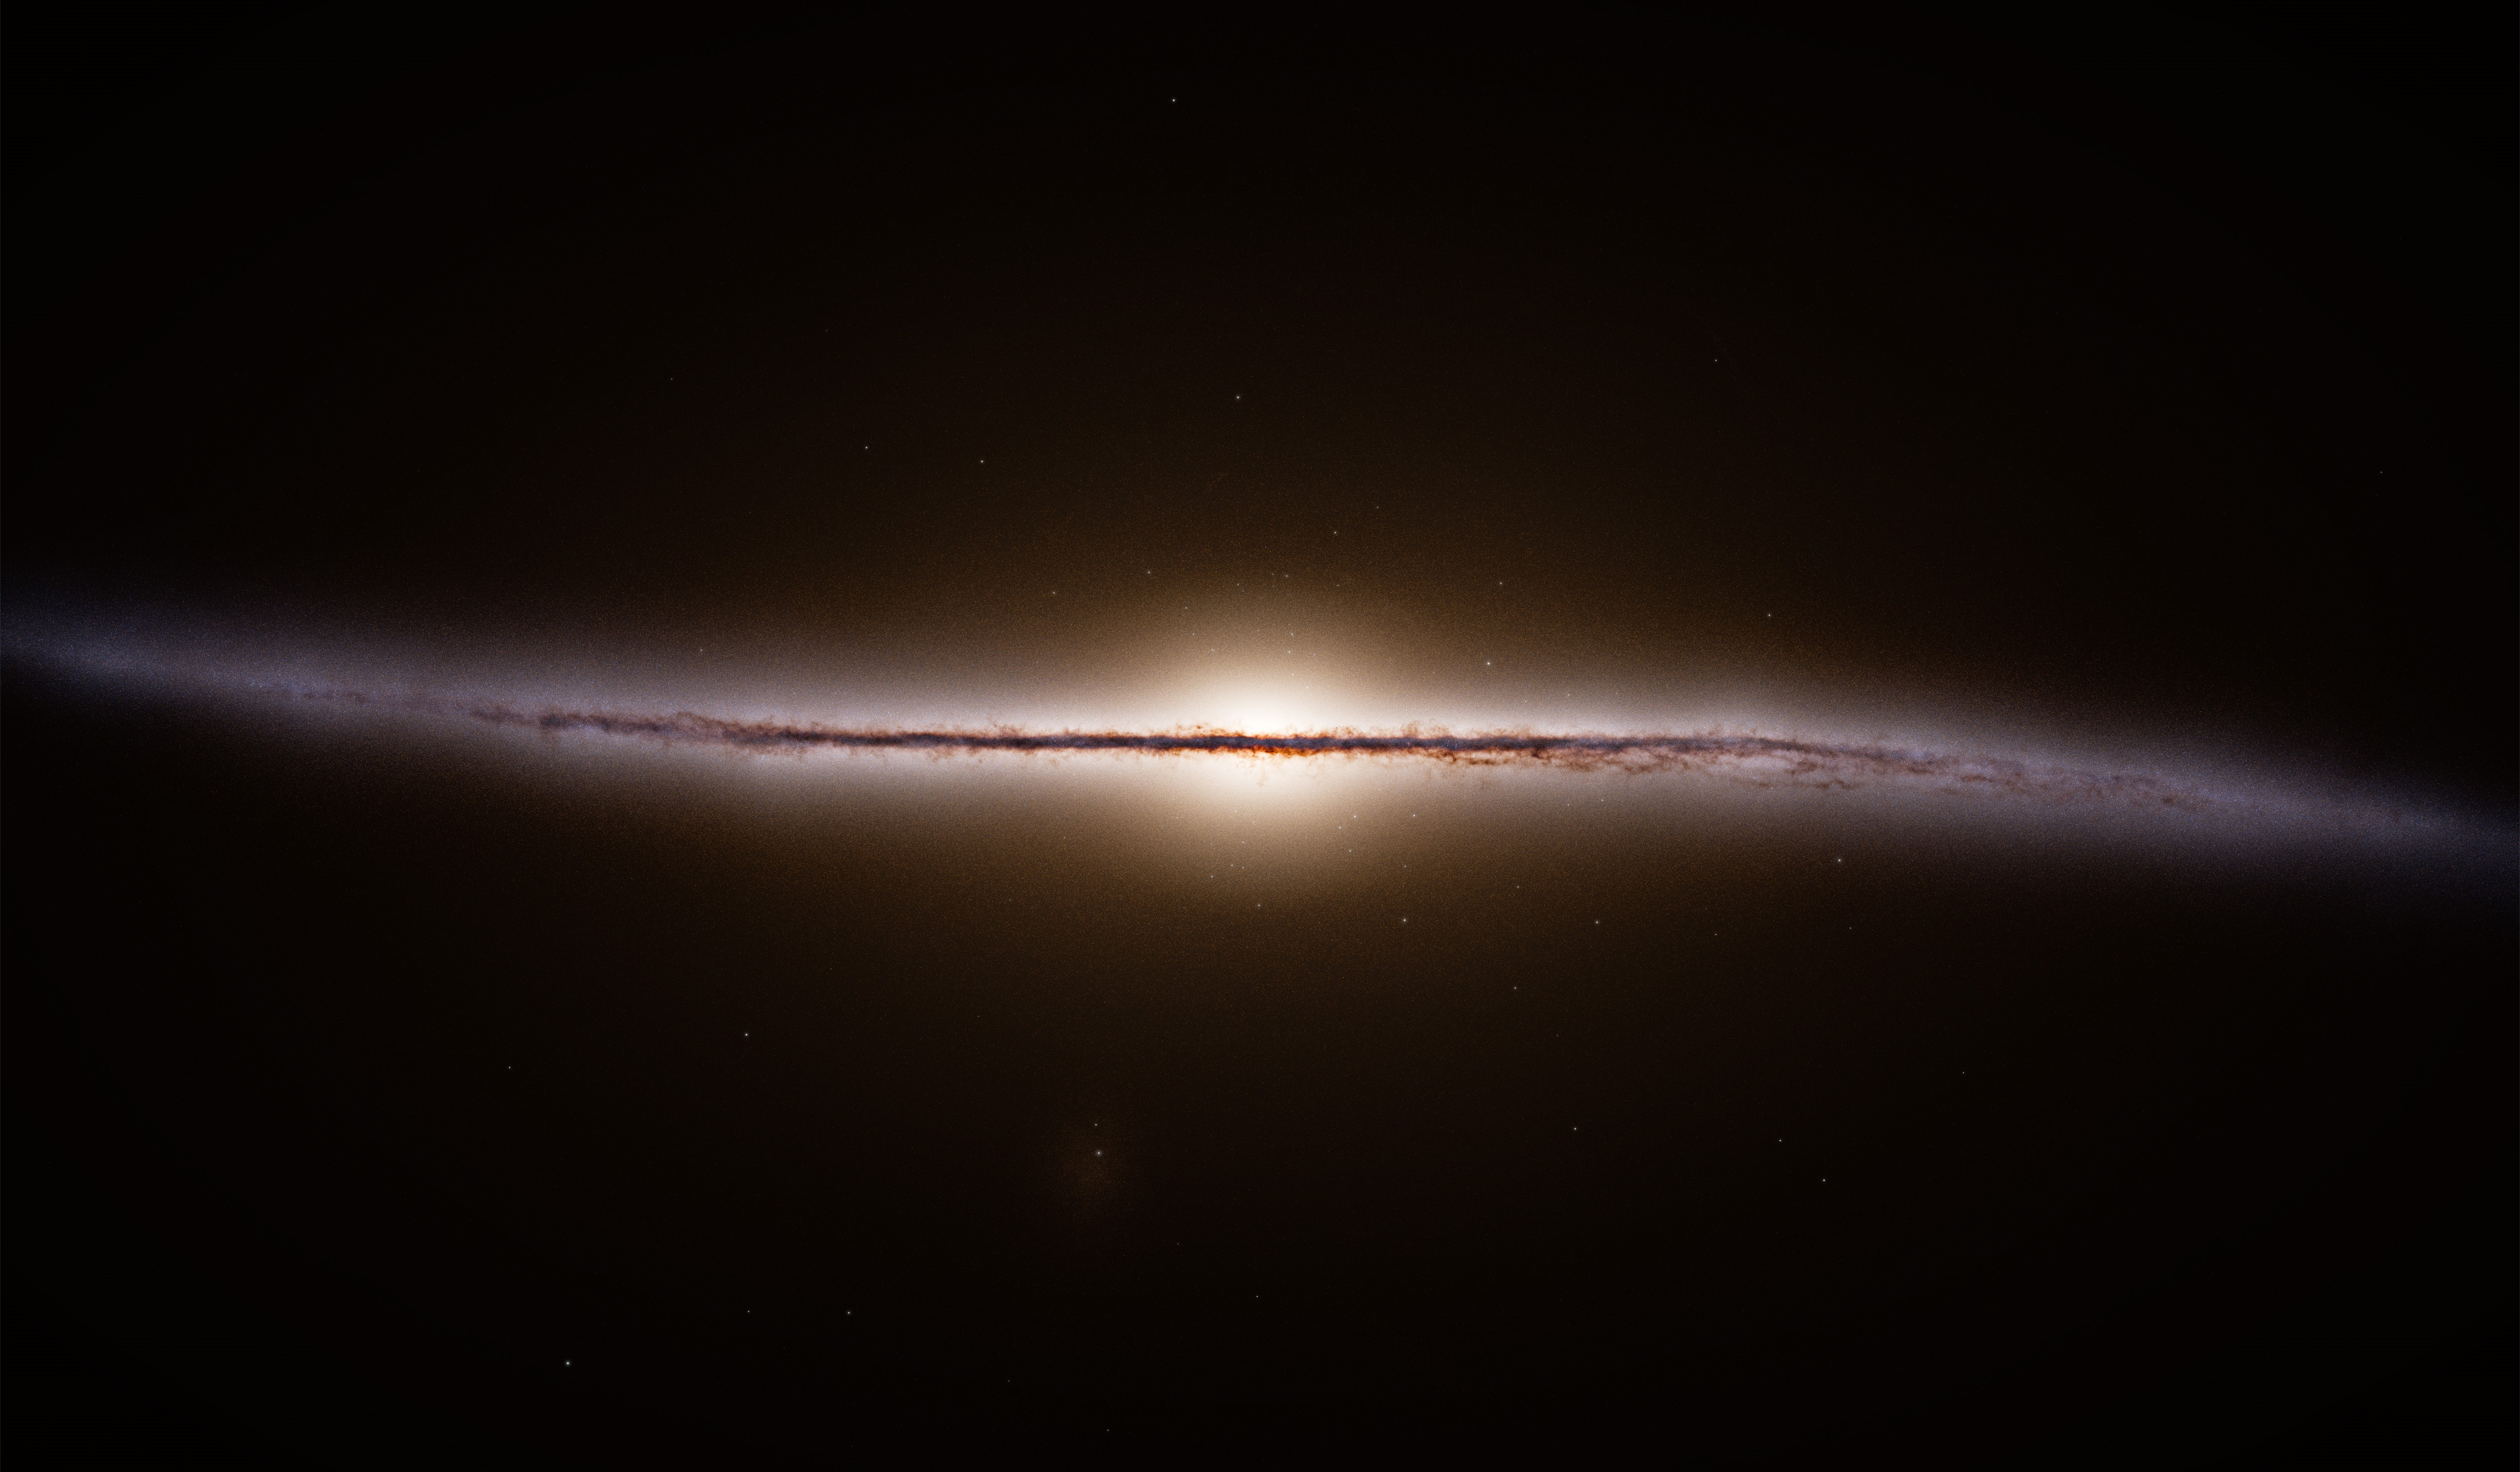
\includegraphics[width=1\linewidth]{revistas/002/imaxes/vialactea.jpg}
    \captionof{figure}{Foto da Vía Láctea polo proxecto Gaia. Fonte: ESA/Gaia/DPAC, por Stefan Payne-Wardenaar}
\end{center}

\paragraph{G:} O ano pasado foi bastante notoria a noticia de que descubrirades un
buraco negro bastante masivo na Vía Láctea. Ti participaras neste achado, cal é
o proceso ata obter os resultados? Sodes partícipes durante todo o proceso do
que se está a descubrir ou analizades os datos a cegas? Que información aportan
estes buracos negros para comprender mellor a galaxia?

\paragraph{A:} Todos os datos de Gaia procésanse masivamente e de xeito
sistemático para depurar resultados espurios e logo facer clasificacións por
categorías, etc. E de cando en vez hai sorpresas ou verdadeiros descubrimentos,
coma no caso deste buraco negro estelar que, de momento, é o máis masivo na
galaxia. No procesado global dos datos traballamos todo DPAC en grupos de
traballo e, dentro destes grupos, un equipo particular foi o que fixo a análise
detallada do descubrimento.

Este tipo de buracos negros (BNs) correspóndense cos estadíos evolutivos finais
das estrelas máis masivas, que morren violentamente en forma de supernovas. E
as estrelas, coa súa evolución, en xeral moldean a evolución química das
galaxias que as conteñen; iso como mínimo. En particular, os BNs son
laboratorios formidables para avanzar no estudo da relatividade xeral e para
poñer a proba o alcance das leis da física. Tamén, para estudar as súas
posibles diferenzas de comportamento cos buracos negros supermasivos dos
centros galácticos, e para progresar no que se coñece como astronomía
multimensaxeiro que combina información electromagnética e de ondas
gravitacionais. Digamos que son obxectos extremos e exóticos de grande
utilidade e bastante versátil en investigación.

\paragraph{G:} Gustaríame preguntar polas colaboracións internacionais. En
proxectos de tan grande escala a participación de grupos de traballo de
diversos países entendo que é imprescindible: é fácil unir a xente de varios
lugares para traballar en equipo ou é un traballo máis independente? Consideras
que hai unha búsqueda de coñecemento e respostas en todo o mundo ou hai países
máis proclives e outros que non prestan tanta colaboración?

\paragraph{A:} Efectivamente, a colaboración internacional, pero a todas as
escalas en realidade, é imprescindible para a consecución de obxectivos. A
astrofísica leva a colaboración científica implícita no ADN, diría eu. Para min
foi case unha das primeiras ferramentas de traballo que aprendín xa na etapa da
especialización, antes do doutoramento.

E canto máis ambiciosos os obxectivos (exploración espacial, vida
exoplanetaria, expansión acelerada do universo...) maiores e máis amplas
colaboracións que tecemos. Da miña experiencia, e até onde eu sei, en
astrofísica colaboramos de todos os xeitos que se precise e por todas as partes
do mundo, unha vez definido o proxecto e os obxectivos que corresponda. Creo
que só así se pode entender o enorme avance desta disciplina e, paralelamente,
do noso coñecemento do universo dende hai pouco máis dun século.

\paragraph{G:} Unha cuestión que se plantexa máis dalgunha estudiante é se a
ciencia é un espazo igualitario, se a búsqueda do coñecemento está exenta de
estereotipos e se en xeral é un espazo afable. Queda camiño por percorrer ou a
situación é positiva ao respecto?

\paragraph{A:} Eu coñezo moitas colegas con recoñecidísimas traxectorias
profesionais, desenvoltas no espazo científico que hai. Ese espazo e tan
igualitario coma o espazo social e laboral no que se inxira. En España hai
arredor dun 30\% de astrofísicas, pero esta porcentaxe é menor nalgúns paises.
E nas universidades españolas hai aproximadamente un 25\% de catedráticas e un
75\% de catedráticos. Creo que estes números indican algo e si quedan aínda
dificultades por superar. Penso que é labor de todos os elementos da sociedade,
a nivel individual e colectivo, esclarecer por que pasa isto e poñerlle
solución.

\begin{center}
    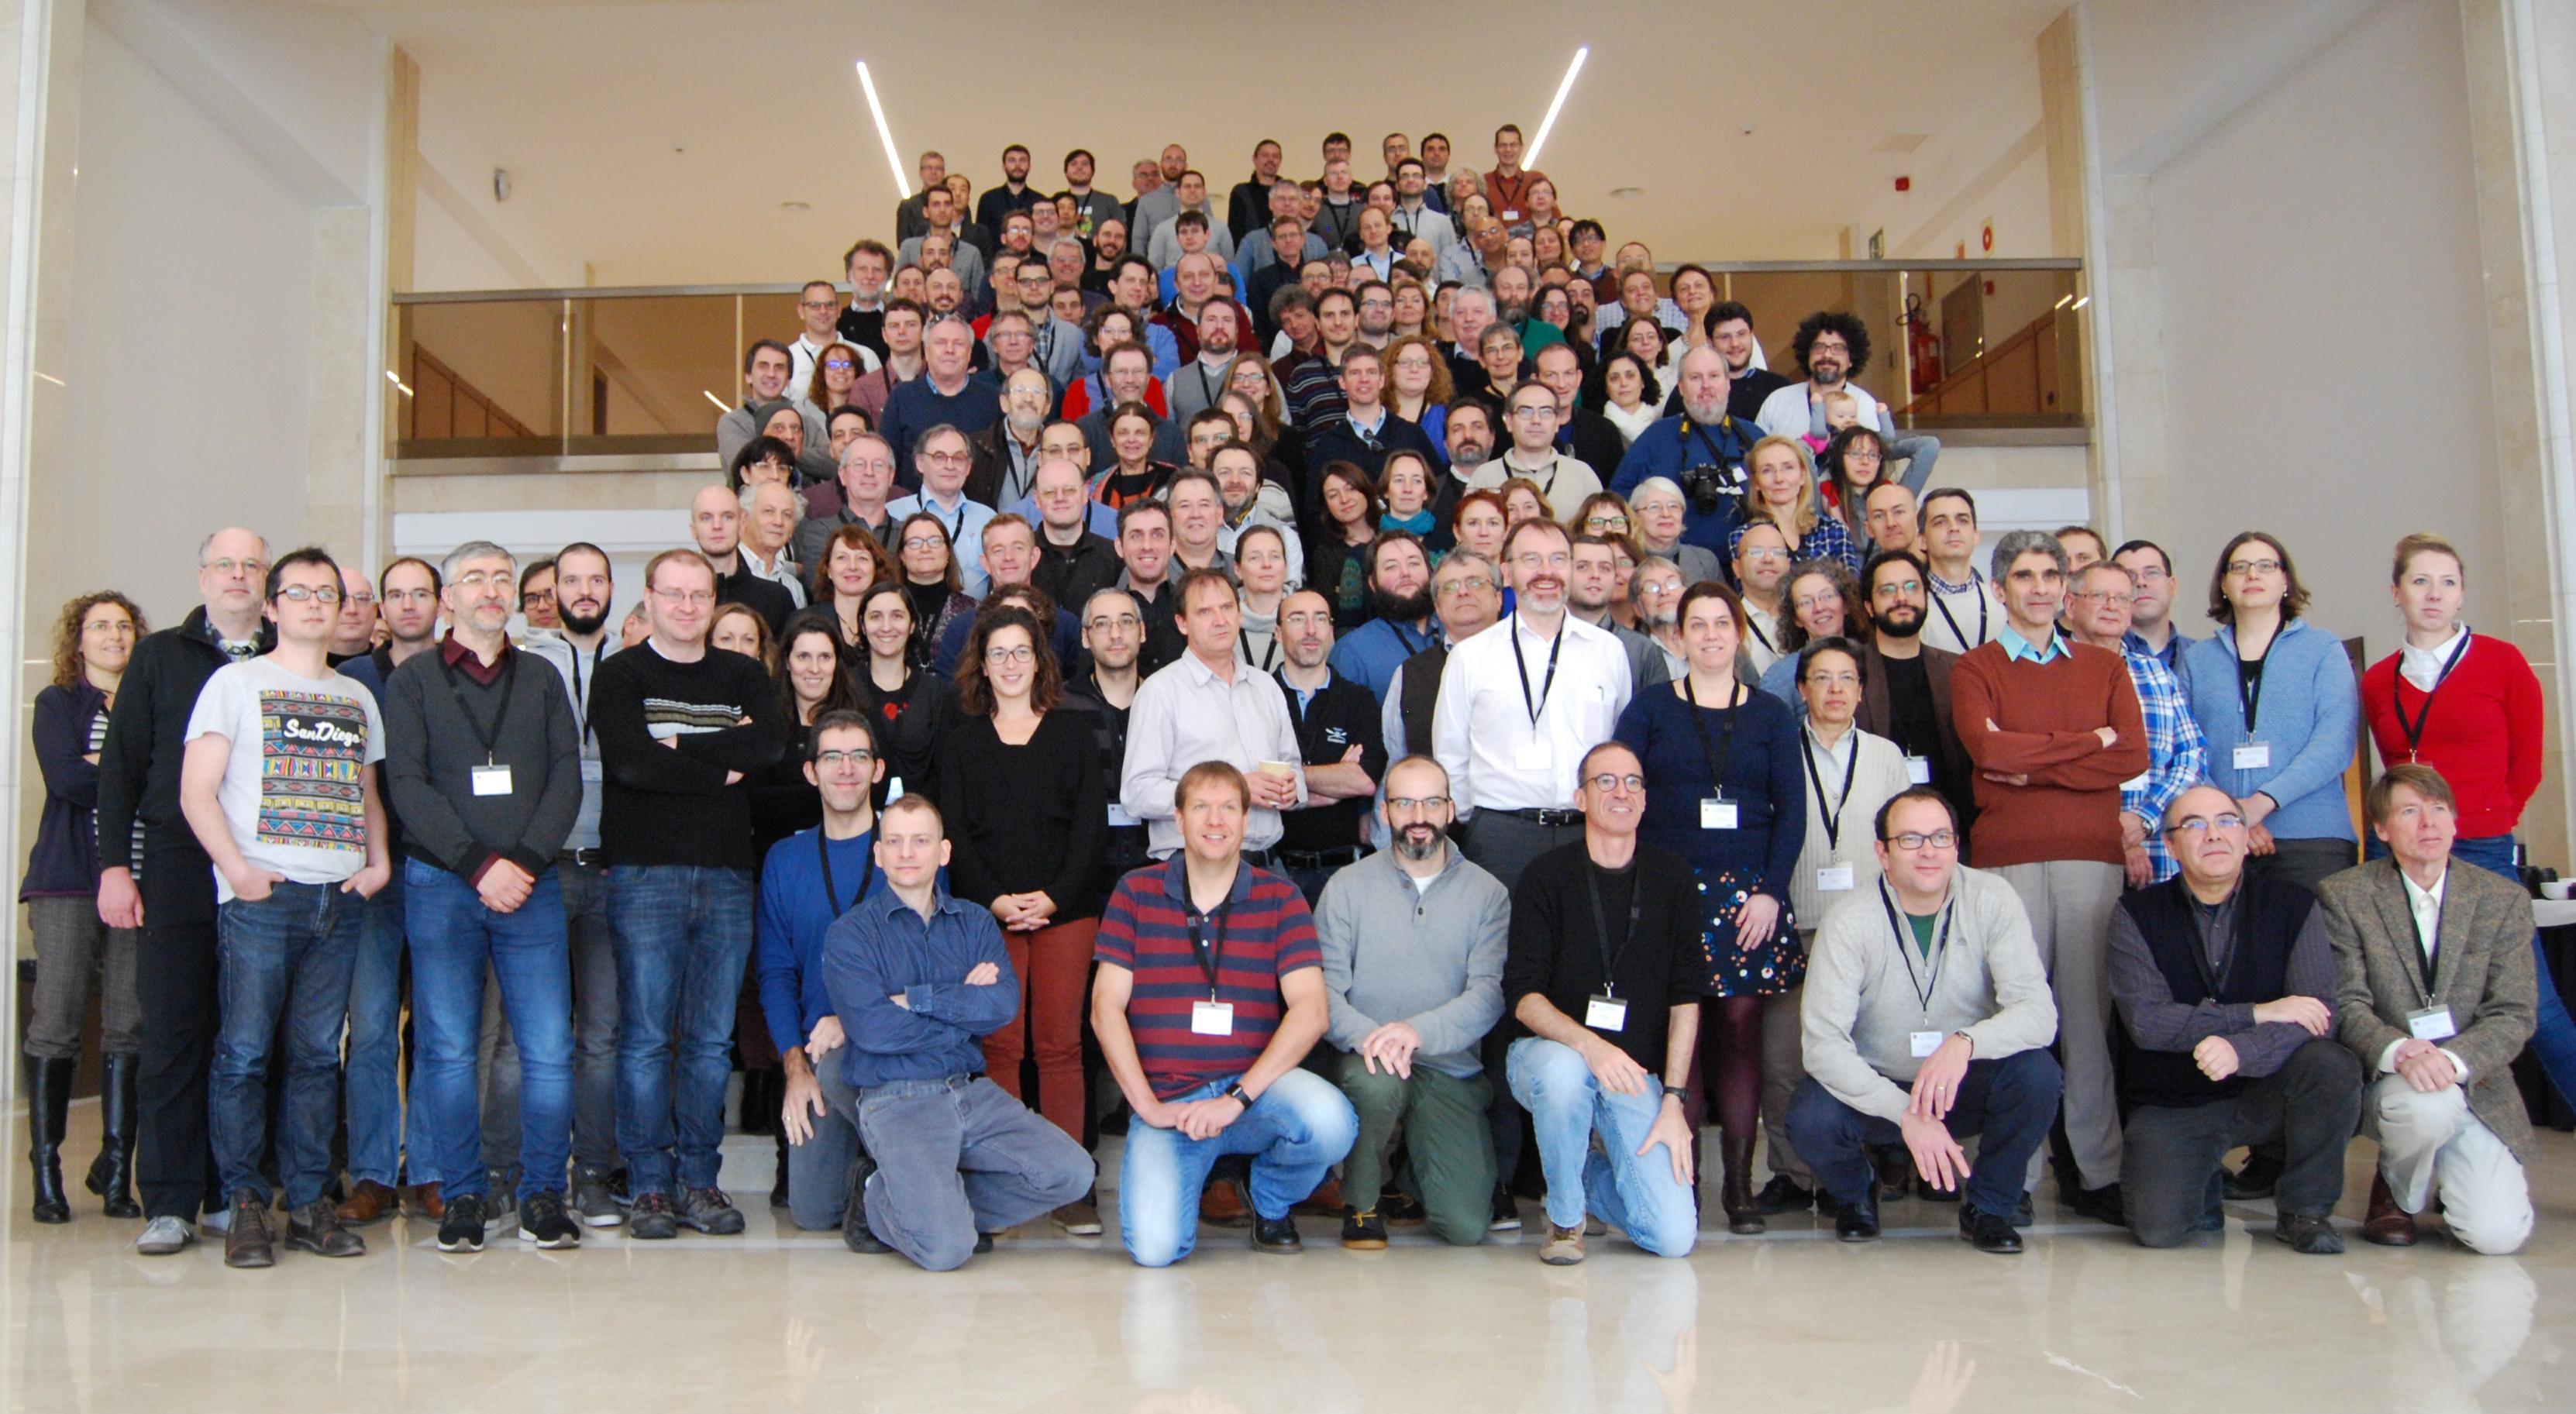
\includegraphics[width=1\linewidth]{revistas/002/imaxes/grupogaia.jpg}
    \captionof{figure}{Participantes da 2ª Reunión do Consorcio DPAC en Sitges, España. Fonte: ESA/Gaia/DPAC}
    %Participants of the 2nd DPAC Consortium Meeting in Sitges, Spain. Image credit:
\end{center}

\paragraph{G:} Nos últimos meses a situación xeopolítica global está cambiando e
as alianzas territorias como a Unión Europea están avanzando a un maior gasto
tecnolóxico, algo que non todo o mundo comprende ou considera necesario. Que
lle dirías a alguén que dubida da importancia de custear proxectos sobre a
exploración espacial? É algo inherente ao ser humano ir en busca de respostas
sobre o Universo ou os intereses residen na utilidade que poida supoñer para os
países?

\paragraph{A:} O universo é todo e abrangue todas as escalas. O investimento en
ciencia e tecnoloxía sempre, antes ou despois, reverte no beneficio das
sociedades que, por este razoamento, son parte do universo. E isto enténdese
mellor se as sociedades teñen un mínimo nivel de cultura científica. Por
exemplo: un software para recoñecer galaxias afastadas é útil para detectar
nódulos difusos de cancro de mama; polo tanto, seguimos investigando as
galaxias, ou gastamos só en recursos médicos? A exploración espacial é
imposible sen as telecomunicacións, e estas son posibles grazas a satélites. Ou
ben, espérase que todo o mundo coñeza El Quijote ou A Gioconda pero que o
obxectivo dun Tokamak sexa producir enerxía limpa e ilimitada por fusión, coma
no interior do Sol, iso a sociedade non ten necesidade de sabelo?

Creo que abondan os exemplos da combinación de perseguir intereses de
coñecemento \textit{per se}, cos de ciencia e tecnoloxía aplicadas. Non son
intereses incompatibles, senón que son beneficiosamente complementarios.

\paragraph{G:} Que valoración farías de como está a astrofísica en España? Cres
que coa incorporación de dous españois ao cadro de persoal de astronautas da
ESA visibilizouse a importancia das misión e investigacións espaciais?

\paragraph{A:} O nivel investigador e tecnolóxico da astrofísica española é moi
alto. Dende que se sentaron as bases dos observatorios de Canarias, Calar Alto
e Sierra Nevada, xunto coa posta en marcha de institutos de investigación
asociados, que hoxe son recoñecidos mundialmente, o avance da astrofísca é
realmente imparable. Polo número e tipo de proxectos, terrestres ou espaciais,
nos que a nosa comunidade está involucrada, dentro e fóra do país, polas
publicacións, pola calidade das teses de doutramento defendidas... por moitos
indicadores, que ademais son parámetros medibles.

Por suposto, é boa nova que a ESA incorpore máis astronautas españois aos seus
equipos, e seguro que iso si contribúe a visibilizar a relevancia das misións e
investigacións espaciais. E espero que tamén contribúa a fomentar novas
vocacións científicas e tecnolóxicas.

\paragraph{G:} Dende a túa experiencia, tes algún consello que poidas compartir
cos estudantes de física e especialmente coas mozas que estén comezando?

\paragraph{A:} O mesmo consello que me deron a min varias mestras e profesores
dende a escola primaria e o instituto, logo investigadores e investigadoras
noutras etapas máis adiante: que o intenten, que non se digan a si mesmos/as
que non van poder con aquilo que queiran conseguir. Ás veces, as cousas non
saen como esperamos, por diversas razóns, así que tamén hai que ter, digamos,
plan B ou C, para continuar no noso camiño.

Pero intentando as cousas nunca quedaremos coa dúbida, ademais de que de todas
as situacións, todas, se pode obter sempre información útil para o presente e o
futuro. Ou, incluso e posiblemente, para reinterpretar o pasado.

\end{multicols}
\end{refsection}
\newpage
\Titular*%
{De onde xorde a ecuación de Schrödinger?}%
{Mauro Garrido Rodríguez}%
{divulgacion}%
{Unha bela relación entre a mecánica clásica, a óptica e a cuántica.}%

\begin{refsection}
\begin{multicols}{2}


Na maioría de libros de texto de mecánica cuántica a ecuación de Schrödinger
introdúcese axiomaticamente; como é posible non dar unha xustificación da pedra
angular da cuántica? Como chegou Schrödinger á súa ecuación? Neste artigo imos
explorar o xeito, elegante e profundo, co que Schrödinger chega a unha das máis
importantes ecuacións da física no seu artigo de 1926, adaptándoo ao lector
para unha exposición máis didáctica.

\subsection*{A analoxía opto-mecánica}

Schrödinger lémbranos como, antes de ser coñecido o fenómeno da difracción da
luz, esta era considerada como transportada por <<raios>>: a luz propagábase en
liña recta nun mesmo medio, e cambiaba a súa pendente ao pasar a outros, mais
mantendo sempre unha propagación rectilínea. Se un físico que só coñecese a
óptica xeométrica (O.X.) quixese explicar a difracción, dinos Schrödinger,
atoparíase con que os raios \textit{xa non serían rectilíneos e influiríanse
uns aos outros dun xeito do máis curioso, en total contradición coas máis
fundamentais leis da óptica xeométrica}. Na macroescala a O.X. pode funcionar,
mais cando os obxectos cos que tratamos vólvense comparables coa lonxitude de
onda da luz (un parámetro que por suposto na O.X. carece de sentido) esta falla
estrepitosamente e temos fenómenos como os de difracción. A raíz disto, e
inspirado no traballo de De Broglie, dinos: \textit{acaso non está un tentado a
investigar se a non-aplicabilidade da mecánica ordinaria a problemas
micromecánicos é quizais do mesmo tipo que a non-aplicabilidade da óptica
xeométrica no fenómeno de difracción ou interferencia?}. Hai acaso unha
formulación da mecánica clásica que teña que ver cun comportamento ondulatorio?
\textbf{Si}, e era coñecida por \textbf{sir William Rowan Hamilton} en 1833.
Este fixouse no parecido do principio de mínima acción mecánico co principio de
Fermat óptico. Lembremos que di cada un:

\begin{itemize}

    \item \textbf{Principio de mínima acción}. Resumidamente, consiste nunha
reformulación da mecánica clásica (a chamada mecánica analítica), onde, de
tódalas traxectorias posibles que pode tomar un partícula, esta só escolle
aquela que fai estacionaria unha determinada cantidade denominada
\textbf{acción} (isto é, que non cambia a primeira orde baixo variacións
pequenas da traxectoria), de xeito que

    \begin{equation}
        \delta S = 0 \rightarrow \frac{d}{dt}\frac{\partial
        \mathcal{L}}{\partial \Dot{q}} - \frac{\partial\mathcal{L}}{\partial q} = 0
    \end{equation}

    onde $\mathcal{L} = T-V$ é o lagranxiano,
$S=\int_{t_0,q_0}^{t,q}\mathcal{L}(q,\Dot{q},t)dt$, e a ecuación que se deriva
do principio de mínima acción é a ecuación de Euler-Lagrange, que é a que rexe
o movemento da partícula, o equivalente a $F=ma$ na mecánica estándar ou
clásica.

    \begin{figure}[H]
       \centering
       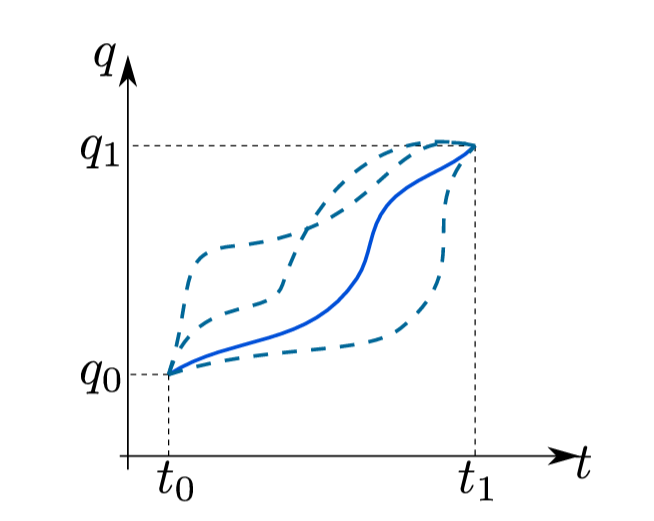
\includegraphics[width=0.7\linewidth]{revistas/002/imaxes/hj2.png}
       \caption{Traxectorias posibles para unha partícula (Fonte: \cite{bahramhouchmandzadeh_2020})}
    \end{figure}

    \item \textbf{Principio de Fermat}. Postula que os raios de luz seguen as
traxectorias de mínimo tempo. Lagrange xeneralizaríao matizando que realmente
as traxectorias que son escollidas son as estacionarias. Ao igual que no caso
mecánico, non sempre se escollen as traxectorias de mínima acción, senón as que
a fan estacionaria. Este principio, de feito, pode facerse equivalente ao
anterior tendo en conta un lagranxiano óptico $\mathcal{L_{op}} = n(s)$ ($n(s)$
é o índice de refracción en cada punto), sendo a nosa condición de <<acción
óptica>> ou <<camiño óptico>> estacionario a seguinte
    \begin{equation}
        \delta S_{op} = \int_A^B\mathcal{L_{op}}ds = 0
    \end{equation}

    Este camiño óptico ten unha interpretación clara: é a distancia que
recorrería a luz no baleiro no tempo que tarda esta en facelo nun medio con
$n(s)$, posto que o índice é unha medida da relación entre as distancias
percorridas nun medio e no baleiro, $n=\frac{c}{v} = \frac{dx_c/dt}{dx_v/dt} =
\frac{dx_c}{dx_v}$. Se resolvemos esta ecuación, atoparemos a \textbf{ecuación
dos raios da óptica xeométrica}.
    \begin{equation}
        \frac{d}{ds}(n\frac{d\vec{r}}{ds})=\nabla n
    \end{equation}

    Así, esta analoxía levou a Hamilton á idea de que o movemento dunha
partícula podería describirse como o análogo a un raio de luz propagándose nun
medio inhomoxéneo ($n(s)$).

    Así, \textbf{de igual xeito que os raios ópticos seguen liñas ortogonais ás
superficies de fase constante} (as frontes de onda da luz), \textbf{as
traxectorias das partículas seguirían liñas ortogonais ás superficies de acción
constante}. A partir desta profunda idea, Hamilton propón que
    \begin{equation}
        p=\frac{\partial S}{\partial q}
    \end{equation}

\end{itemize}

É dicir, que a variación da acción coa posición (xeneralizada) dá lugar ao
momento (xeneralizado) das partículas, que polo tanto se moven ortogonalmente
ás superficies de acción constante.

\begin{figure}[H]
   \centering
   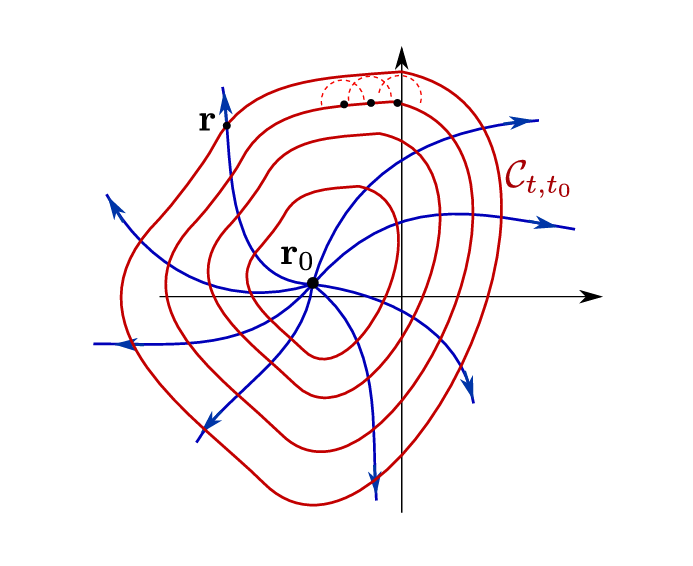
\includegraphics[width=0.6\linewidth]{revistas/002/imaxes/hj1.png}
   \caption{Relación entre as superficies de fase constante e os raios (Fonte: \cite{bahramhouchmandzadeh_2020})}
\end{figure}

Se combinamos este feito co principio de mínima acción, pasando primeiro polas
\textbf{ecuacións canónicas} (reformulación da de Euler-Lagrange facendo o
cambio de dependencia $\Dot{q}\rightarrow p$, onde agora o papel de
$\mathcal{L}$ faino $\mathcal{H}$, o Hamiltoniano), atopamos a ecuación de
\textbf{Hamilton-Jacobi}.

\begin{equation}
    \frac{\partial S}{\partial t} + \mathcal{H}(q,\frac{\partial S}{\partial q},t) = 0
\end{equation}

Esta ecuación, aínda que non o pareza, é clave para entender a ecuación de
Schrödinger. Imos reescribila e ver o caso máis simple para entendela mellor, o
dunha partícula de masa $m$ movéndose nun potencial $V(x,y,z)$, de xeito que
$\mathcal{H}=E=T+V=\frac{1}{2m}(p_x^2+p_y^2+p_z^2) + V(x,y,z)$. Se incluímos
este hamiltoniano na ecuación de Hamilton-Jacobi, e tendo en conta a suposición
de Hamilton $p=\frac{\partial S}{\partial q}$ atopamos que

\begin{equation}
    \frac{\partial S}{\partial t} + \frac{|\nabla S|^2}{2m} + V(x,y,z)=0
\end{equation}

Para simplificar aínda máis esta expresión consideremos un hamiltoniano
independente do tempo, de xeito que obteñamos unha ecuación para partículas con
enerxía constante. Isto determinará a dependencia temporal da acción

\begin{equation}
    \frac{\partial S}{\partial t} = -\mathcal{H} \rightarrow
    \boxed{S=(E)t + f(x,y,z)}
\end{equation}

Deste xeito, executando a derivada temporal de $S$, a ecuación de
Hamilton-Jacobi queda reducida a

\begin{equation}
    |\nabla S| = \sqrt{2m(E-V)}
\end{equation}

Posto que a enerxía cinética é $T=E-V$, isto non é máis que

\begin{equation}
    |\nabla S| =  |\vec{p}| \rightarrow \boxed{\nabla S = \vec{p}}
\end{equation}

O gradiente da acción, perpendicular ás traxectorias, é o momento da partícula.
Esta é a ecuación dos raios-mecánicos, é dicir, das traxectorias, de enerxía
constante.

\subsection*{A analoxía opto-mecano-cuántica}

Schrödinger é consciente de que ata aquí non hai nada novo. O que el propón é
tomarse esta ecuación en serio. Se realmente esta é o equivalente á ecuación
dos raios da O.X., e a óptica é en realidade ondulatoria, emerxendo estes
delas, por que non facer o mesmo para as partículas, para as súas traxectorias?
Tomándonos en serio a analoxía, a ecuación de Hamilton-Jacobi asócialles ás
partículas unha fase, a acción, que debe de ser a fase dunha onda. \textbf{Se a
luz cumpría unha determinada ecuación de ondas, que ecuación de ondas cumprirá
unha partícula material?}

Antes de chegar a ela, temos que ter en claro que tipo de onda é a que ten a
fase da ecuación de Hamilton-Jacobi: posto que provén de esixir unha fase
estacionaria, pódese probar moi facilmente que é equivalente á \textbf{ecuación
da \textit{eikonal}} da óptica, que é válida para \textbf{ondas
localmente planas}, é dicir, ondas cunha variación de fase suave, con frontes
de onda localmente planas.

\begin{figure}[H]
   \centering
   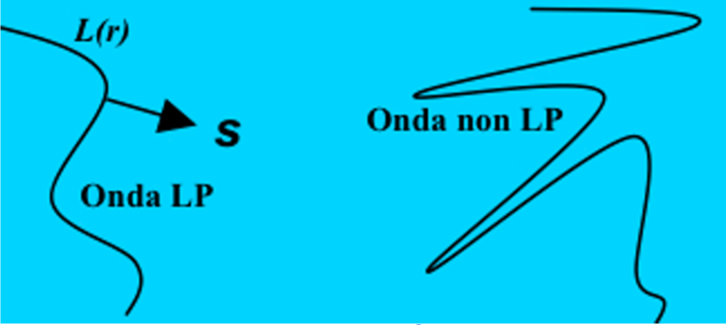
\includegraphics[width=0.7\linewidth]{revistas/002/imaxes/hj3.png}
   \captionof{figure}{Ondas localmente planas (Fonte: \cite{apuntes_optica_2})}
\end{figure}

Na mecánica clásica as únicas ondas consideradas serán localmente planas, que dan
solucións exactas para as traxectorias; pero, en mecánica cuántica, ao igual
que pasaba coa óptica ondulatoria e coa O.X., poderemos ter moitas máis
posibilidades de ondas, \textbf{que darán lugar a movementos inexplicables
mediante o concepto de raios, é dicir, de traxectorias}.

Así, antes de pasar á ecuación de Schrödinger, poremos a proba este concepto de
ondas asociándolle á función de ondas $\Psi$ (o que ondula, cuxo significado
descoñecemos, análogo ao campo electromagnético da luz) dunha \textbf{onda
localmente plana} (polo comentado de que a ecuación de Hamilton-Jacobi só
aplica a estas) a acción $S = Et + f(x,y,z)$ como fase (lembremos que isto
implica E=cte), recordando que debe cumprir $\nabla S=\vec{p}\rightarrow \nabla f(x,y,z) = \vec{p}$. Así,
\begin{equation}
    \Psi = A(x,y,z)e^{i(\frac{S}{B})} = A(x,y,z)e^{i(\frac{E}{B}t + f(x,y,z)/B)}
\end{equation}

onde $B$ é unha constante que permite que o que entra na exponencial sexa
adimensional. Esta é a clase de ondas que corresponden á ecuación de
Hamilton-Jacobi, ondas localmente planas de $E=cte$ cuxas frontes son moldeadas
por $f(x,y,z)$.

Schrödinger di: \textit{un non pode resistir a tentación de supor que $B$ sexa
unha constante universal, porque nese caso}, facendo $B=\hbar$, a frecuencia
desta onda é

\begin{equation}
    \omega=\frac{E}{\hbar} \rightarrow \boxed{E=\hbar \omega}
\end{equation}

A famosa relación de De Broglie enerxía-frecuencia!

\subsection*{A ecuación de Schrödinger}

Para o caso simple que estamos tratando da partícula unidimensional,
Schrödinger propón que $\Psi$ cumpre unha ecuación de ondas ordinaria

\begin{equation}
        \frac{\partial^2 \Psi}{\partial x^2} =
        \frac{1}{u^2}\frac{\partial^2 \Psi}{\partial t^2}
\end{equation}

Agora, asume que estas ondas se moven cunha velocidade de fase dada pola
ecuación de Hamilton-Jacobi ($p=\frac{\partial S}{\partial x} \rightarrow v=
\frac{1}{m} \frac{\partial S}{\partial x}$), asumindo tamén solucións de
enerxía constante (polo tanto, a parte temporal da acción será $S=Et$), o cal
converte a esta ecuación de ondas na \textbf{ecuación de Schrödinger
independente do tempo}. Así,

\begin{equation}
    \boxed{
        -\frac{\hbar}{2m}\frac{\partial^2\Psi}{\partial x^2} +
        V(x,y,z)\Psi = E\Psi
    }
\end{equation}

Que, polo dito anteriormente, é unha ecuación só válida para ondas asociadas a
partículas de enerxía constante. Fixémonos en que agora non se asume unha onda localmente
plana (a ecuación non foi obtida con esa premisa), co que esta ecuación é
valida para ondas arbitrarias que corresponderían ás <<traxectorias>>
cuánticas. Plasmar a importancia desta ecuación neste artigo é unha tarefa
colosal que non pode abarcarse aquí, mais o que fai Schrödinger inmediatamente
despois de conseguila é aplicala ao átomo de Hidróxeno, reproducindo así os
valores cuantificados dos niveis de enerxía, explicando o átomo de Bohr. É de
interese resaltar o feito de que se poidan obter tantos resultados sen darlle á
$\Psi$ unha interpretación aínda.


\nocite{schrodinger.e_1926}
\nocite{schrodinger.e_1926_2}
\nocite{hamilton_optico_mechanical}
\nocite{hamilton_jacobi_equation}

\printbibliography

\end{multicols}
\end{refsection}
\newpage
\Titular%
{O Teorema de Bohr-Van Leeuwen: o segredo está na cuántica}%
{Luis Arcas Morcillo}%
{divulgacion}%
{Da imposibilidade clásica do magnetismo.}%


\begin{refsection}
\begin{multicols}{2}


\textit{Classical magnetism is fake}. Estou seguro de con este artigo a
polémica está servida. Gústame imaxinar que os nosos prezados lectores
dividiranse en dous bandos. Uns entrarán en pánico e ante a afirmación anterior
quererán abolir o estudo da magnetostática clásica en tódalas facultades do
país. Outros, quizais máis cínicos (e con razón), pensarán que ten moito
sentido que o magnetismo é unha consecuencia cuántica. A fin de contas, todo
fenómeno a escala atómica debe rexer as leis da mecánica cuántica. Non
obstante, este feito non era para nada coñecido no comezo do século XX, onde
comeza a nosa historia. Abrochade os vosos cintos, porque avecíñanse curvas.

\subsection*{O magnetismo previo ao átomo}

Supoño que os inicios da teoría do magnetismo son coñecidos pola maioría, pero
en resumidas contas aconteceu máis ou menos así:

Dende tempos inmemoriais, antigas civilizacións xa coñecían a ferrita, un
mineral que posuía a fascinante propiedade de atraer metais. Séculos despois,
científicos renomados como Faraday, Lenz e Maxwell contribuíron ao primeiro
formalismo dunha teoría que actualmente coñecemos como electromagnetismo (EM),
nunha formulación de campos que é de moita utilidade para sentar as bases da
electrodinámica. Así, o ser humano era agora capaz de simular as propiedades da
ferrita a partir de cargas eléctricas en movemento nun circuíto, mostrando o
vínculo profundo entre a electricidade e os imáns. No entanto, quedaba pendente
unha cuestión: por que hai materiais que presentan campos magnéticos propios
permanentes? Que propiedades ten a ferrita e outros materiais presentes na
natureza para actuar como imáns naturais?

O descubrimento do átomo e das primeiras partículas subatómicas tivo unha
grande relevancia non só a nivel experimental, senón tamén conceptual. Os
electróns e protóns teñen carga igual e de signo oposto, pola súa contra, as
masas son distintas, onde claramente é maior a masa do protón. Entón, ten
sentido pensar que estas partículas cargadas en particular, e os átomos en
xeral, son susceptibles individualmente á actuación de campos
electromagnéticos. A enerxía adquirida pola presenza dun campo magnético pode
describirse a partir do momento magnético da partícula cargada: 
\begin{equation}\label{ec.: energia_momento}
    \vec \mu = \frac{1}{2m}(\vec r\times q\vec v)\Longrightarrow E =
    -\vec \mu\vec B = -\mu_zB.
\end{equation}

O signo negativo corresponde ao feito de que a enerxía minimízase cando o
momento magnético $\vec \mu$ está aliñado co campo: $E=E_\mathrm{mín}
\Leftrightarrow \vec \mu \parallel \vec B \Leftrightarrow \vec \mu=\mu \hat z$. 

Sen entrar en moitos detalles, o comportamento dos momentos magnéticos dos
átomos individuais fronte a campos magnéticos permitiríanos describir o
material. Se tódolos momentos están aliñados entre eles, falamos de
\emph{ferromagnetismo}: o material presentaría un comportamento de imán natural
cando se introduce un campo magnético. Se os momentos magnéticos individuais
están desaliñados, de tal xeito que aparentemente opóñense ao campo externo,
falamos de \emph{diamagnetismo}. Sen embargo, se a interacción parece favorable
á dirección do campo, falaremos de \emph{paramagnetismo}.

\subsection*{Langevin e o primeiro modelo atómico do paramagnetismo}

En 1905, o físico francés Paul Langevin foi o primeiro en presentar un modelo
que fose capaz de explicar a escala atómica o comportamento dos distintos
materiais fronte a campos magnéticos. Actualmente estúdase como a \emph{teoría
semiclásica do paramagnetismo} \cite[Sec. 2.1.4.]{blundell.s_2001}. Langevin
propoñía que os átomos tiñan un momento magnético constante apuntando a certa
rexión do espazo segundo a distribución de Boltzmann:

\begin{equation}\label{ec.: bvl_boltzmann}
    dP = \frac{1}{Z}e^{\frac{E}{k_B T}}d\Omega,\,\, Z
    =\int_{0}^{2\pi}\int_{0}^{\pi}e^{\frac{E}{k_B T}}d\Omega,
\end{equation}

onde $d\Omega = \sin(\theta)d\theta d\phi$ é a diferencial do ángulo sólido.
Así, dados $N$ átomos dun material lineal nun volume $V$, a magnetización
resultante do material é a siguiente:

\begin{equation}\label{ec.: blv_langevin}
    M = \frac{N}{V} \int\mu_zdP = \frac{N}{V}\cdot
    L\left(\frac{\mu B}{k_B T}\right),
\end{equation}

onde $L(y) = \coth(y)-y^{-1}$ é a función de Langevin. Dous anos máis tarde, o
tamén francés Pierre Weiss propuxo outro modelo que correxía o de Langevin e
introducía o comportamento ferromagnético de diversos materiais na teoría.

\subsection*{As disertacións de Bohr e Van Leeuwen. Unha nova teoría.}

Os problemas non tardarían en chegar. Xa por 1911, un novo Niels Bohr puxo en
dúbida a teoría de Langevin, achando unha contradición infranqueable se
soamente se empregaban técnicas de Mecánica Estadística. Anos máis tarde, unha
estudante da Universidade de Leiden, chamada Hendrika Johanna van Leeuwen
disertaría sobre o mesmo tema na súa tese doutoral, chegando ás mesmas
conclusións que Bohr. Vexamos cal foi o seu razoamento e as conclusións finais
\cite[Sec. 1.2.2.]{blundell.s_2001}.\\

Consideremos unha mostra paramagnética de $N$ átomos, todos coa mesma masa, no
seo dun campo magnético. Consideraremos exclusivamente o momento debido aos
electróns, sendo o resultado xeral para outras partículas cargadas. Tense entón
que cada electrón ten un momento magnético:
$$\vec \mu = \frac{-e}{2m} ({\vec r}\times \dot {\vec r}) \Rightarrow
\mu_z=\sum_{i=1}^{3N}a_i(q_1,\dots,q_{3N})\dot q_i.$$

É dicir, o momento magnético total nunha dirección (a dirección do campo $\vec
B$) é unha función explícita das velocidades nas coordenadas xerais.

Consideremos ademais que o noso sistema conserva a súa enerxía, de tal feito
que o total correspóndese co hamiltoniano, función de coordenadas xerais, $\vec
q$ e os seus momentos canónicos conxugados, $\vec p$. Para un sistema sometido
a un campo electromagnético caracterizado polos potenciais $(\phi,\vec A)$,
dáse o seguinte hamiltoniano :
\begin{equation}\label{ec.: bvl_hamiltoniano}
    E=H(\vec q,\vec p) = \frac{1}{2m}\sum_{i=1}^N (\vec p_i - e\vec
    A_i)^2 + e\phi(q_1,...,q_{3N})
\end{equation}

Podemos promediar os seus momentos magnéticos para achar a enerxía promedio do
sistema $\braket{E} = -B\braket{\mu_z}$. Segundo a Mecánica Estadística
\eqref{ec.: bvl_boltzmann} e o modelo de Langevin \eqref{ec.: blv_langevin},
podemos calcular este promedio a partir da función de partición $Z$ da mostra:
\begin{equation}\label{ec.: bvl-mec_est}
    \braket{\mu_z} = \int \mu_z\, dP = \frac{1}{Z}\int e^{-\beta
    H(\vec q,\vec p)} \, d^N(\vec q, \vec p),
\end{equation}

onde $\beta^{-1} = k_B T$. Recordando as relacións de conxugación canónica no
formalismo hamiltoniano, temos que $\dot q_i = \frac{\partial H}{\partial
p_i}$, e polo tanto o promedio cumpre que:
\begin{equation}
    \braket{\mu_z} = \frac{1}{Z}\iint\sum_{i=1}^{3N} a_i
    (q_1,...,q_{3N}) \frac{\partial H}{\partial p_i}e^{-\beta
    H}d^{3N}(\vec q,\vec p).
\end{equation}

No entanto, se integrarmos na totalidade do espazo de fases, veremos que o
promedio é igual a cero\footnote{É un bo exercicio para o lector facer os
cálculos, aquí vai unha pista: separe a integral múltiple no producto das
integrais na posición $\vec q$ e o seu momento $\vec p$. O integrando
dependente de $\vec p$ é impar, e polo tanto a integral anúlase.}. Deste modo,
baixo a acción do campo, en promedio estadístico hai tantos momentos aliñados
coma desaliñados: a mostra é diamagnética.\\

En resumidas contas, de ser pola teoría clásica, non habería magnetismo
posible, nunha clara contradición coa realidade experimental. Así, era
necesaria unha nova teoría que fose capaz de explicar a presenza do magnetismo
na natureza. Segundo \citet[pp. 354-355]{van-vleck.jh_1977}, foi este feito o
que motivou a Bohr a introducir a cuantización do momento angular orbital do
electrón ao redor do núcleo de hidróxeno para plantexar o seu famoso modelo
atómico. Así, un pode afirmar que o nacemento da cuántica está moi vinculado ao
magnetismo atómico. 

\subsection*{Conclusións}

En definitiva, aínda que a teoría de Maxwell é moi útil para explicar fenómenos
electromagnéticos clásicos coma a indución magnética ou mesmo a luz (o que
podería dar para outro artigo), a imposibilidade de explicar o fenómeno do
paramagnetismo pon de manifesto que fai falla unha teoría máis completa, que
teña presente o comportamento propio dos átomos. É dicir, que, unha vez máis, a
cuántica está aquí para salvarnos da catástrofe. Un desenvolvemento máis
completo do rol da cuántica no magnetismo pode cursarse na asignatura de
Nanomagnetismo e Nanotecnoloxía desta facultade.

\printbibliography

\end{multicols}
\end{refsection}
\newpage
\Titular%
{O misterio da materia escura}%
{Pablo Falgueras Casarejos}%
{divulgacion}%
{O descubrimento da maior parte da materia do universo e o enigma da súa composición.}%


\begin{refsection}


\begin{multicols}{2}


Dende os anos trinta do século XX sabemos que no universo hai algún tipo de materia invisible aos nosos instrumentos debido aos efectos que esta ten no seu entorno. Un dos primeiros en obter probas firmes sobre este feito foi o físico Fritz Zwicky no ano 1933 mentres estudada o Cúmulo de Coma, un cúmulo formado por unhas mil galaxias na constelación de Coma Berenices, a algo máis de 300 millóns de anos luz. Zwicky mediu as velocidades das galaxias do cúmulo e atopou que eran moito maiores do esperado só tendo en conta a materia visible, de feito, chegaban a superar a velocidade de escape estimada para o cúmulo. En consecuencia, propuxo que debía existir algún tipo de “materia escura” que non podiamos observar responsable do movemento anómalo das galaxias. Non obstante, este achado caeu no esquecemento ata catro décadas despois. Hoxe en día sábese que Zwicky sobreestimou a cantidade de materia escura porque non tivo en conta o gas intergaláctico (aínda non descuberto), o cal aporta a maior parte da masa do cúmulo. 

Xa na década dos 70, a astrónoma Vera Rubin xunto con Kent Ford, analizando a velocidade de rotación de estrelas individuais en galaxias espirais, atoparon o mesmo resultado que Zwicky nas galaxias do Cúmulo de Coma corenta anos antes. A velocidade das estrelas era demasiado alta: en vez de diminuír coa distancia, mantíñase aproximadamente constante. De novo, Rubin pensou que existía máis materia da visible, a cal se acumulaba na rexión exterior (halo) das galaxias. As estimacións da cantidade de materia escura suxerían que podía ser ata dez veces máis abundante que a materia ordinaria (ou bariónica, formada por barións).

Ao longo dos anos, presentáronse novas probas que apuntan á existencia desta materia escura. Por exemplo, estudando a velocidade do gas das galaxias, e non a velocidade das súas estrelas, pódese apreciar unha maior anomalía nela. Isto débese a que o gas exténdese máis aló na periferia da galaxia que as estrelas, aínda que tardou en ser descuberto porque emite principalmente en raios X debido á súa alta temperatura. Outros obxectos do halo galáctico cuxa velocidade presenta a mesma irregularidade son os cúmulos globulares, cúmulos moi antigos formados por decenas ou centos de miles de estrelas.

Por outra banda, dende a publicación da teoría da relatividade xeral de Einstein sábese que unha masa deforma o espazo-tempo, polo que pode curvar a traxectoria da luz producindo un fenómeno coñecido como lente gravitacional. Esto prodúcese cando un obxecto masivo (unha galaxia ou cúmulo de galaxias, por exemplo) interponse entre unha fonte de luz (outra galaxia distante) e o observador. Se é o caso, pódese observar a galaxia distante distorsionada debido ao efecto de lente gravitacional do corpo interposto. Estudando como ese corpo curva a traxectoria da luz pódese estimar a cantidade e distribución de masa que produce a lente gravitacional. Grazas a isto, obsérvase que unicamente a materia bariónica non podería producir as lentes gravitacionais estudadas, senón que é necesaria a presencia de máis masa para conseguilo.\\

\begin{center}
    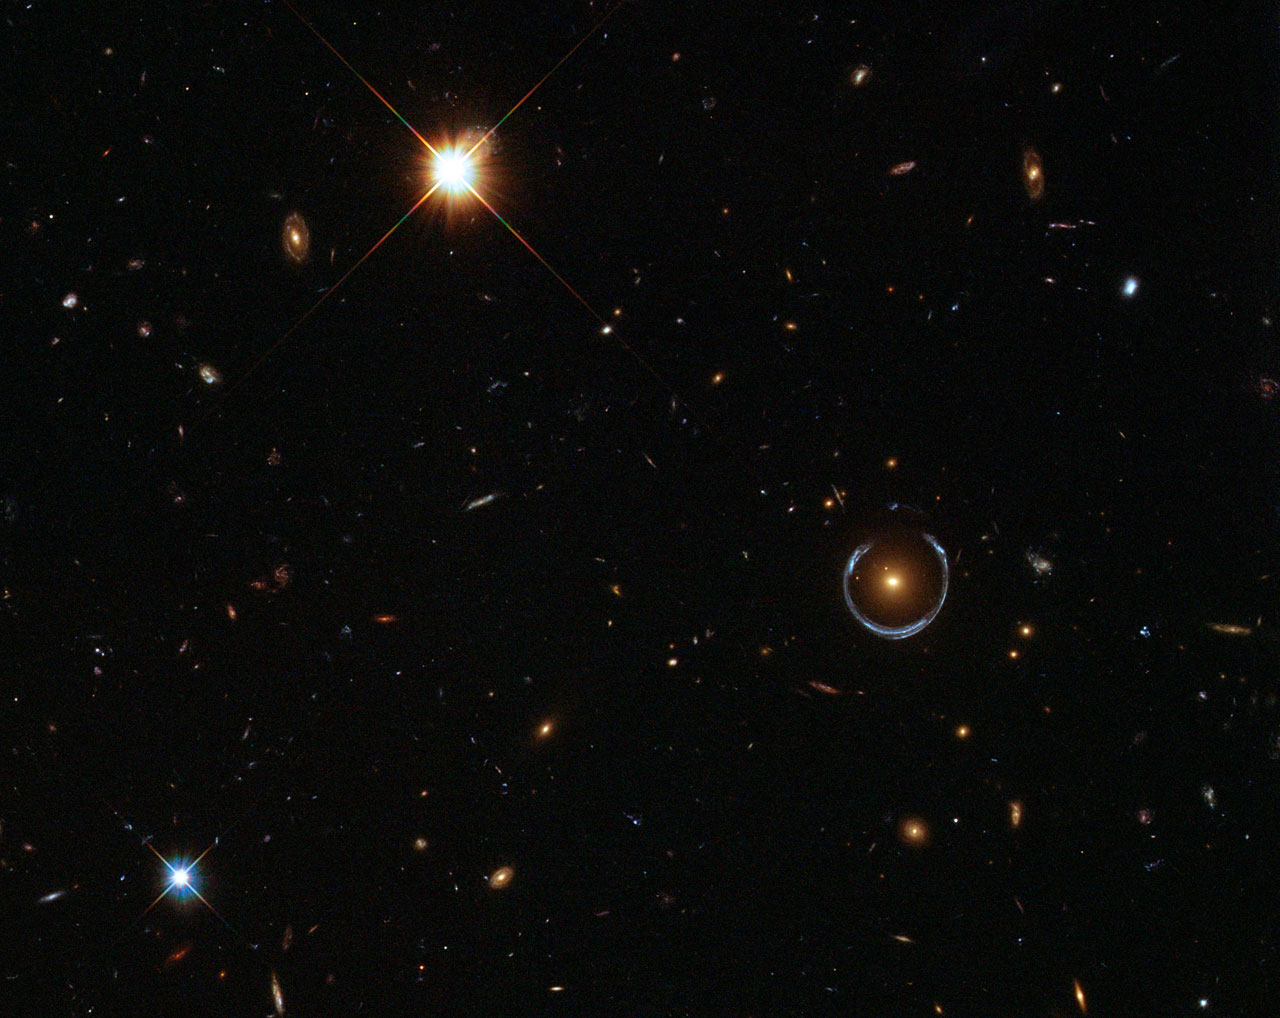
\includegraphics[width=0.9\linewidth]{revistas/002/imaxes/materiaescura1.png}
    \captionof{figure}{LRG 3-757 ou a “ferradura cósmica”, un exemplo das lentes gravitacionais coñecidas como aneis de Einstein \cite{hubbleNASA}.}
\end{center}


Outra proba provén da radiación do fondo cósmico de microondas (Cosmic Microwave Background, CMB, en inglés), radiación emitida durante a chamada “recombinación” uns 380 000 anos despois do Big Bang. Analizando as fluctuacións de temperatura do CMB estímase que a dendisade de materia (escura e ordinaria) do universo atópase en torno ao 32\% da súa densidade crítica, o cal está en perfecto acordo coas observacións, das que se obtén que a materia bariónica supón un 5\% da densidade crítica e a materia escura un 27\%. Por certo, pénsase que a contribución da “enerxía escura” (non materia!) é igual ao 68\% restante, polo que a densidade do universo sería igual á súa densidade crítica e a xeometría deste sería plana.

Sobre as súas características, sábese que a materia escura debe de ser “fría”, é dicir, que a velocidade das súas partículas é moito menor que a velocidade da luz. Se non fose así, o colapso gravitatorio da materia no universo temperán tería sido menos eficiente e non existiría a estrutura a gran escala actual. Tamén debe ser estable, porque a cantidade de materia escura actual debe de ser aproximadamente a mesma que a do universo temperán. Ademais, a materia escura non interacciona coa materia bariónica nin consigo mesma (a excepción da gravidade) ou o fai de forma moi débil. Un claro exemplo preséntase noutro cúmulo de galaxias, o denominado Cúmulo Bala. En realidade, trátanse de dous cúmulos en colisión, os cales xa se atravesaron hai millóns de anos. A partir de observacións en raios X, apréciase que o gas intergaláctico (en vermello na Figura 2) está rezagado respecto aos cúmulos, o cal prodúcese pola fricción das nubes de gas  ao chocar. O interesante é que debido aos efectos de lente gravitacional pódese saber a distribución de materia escura (en azul), que si está superposta ao cúmulo (non rezagada). Isto quere dicir que cando os cúmulos colisionaron, a materia escura atravesou as nubes de gas e a si mesma sen apenas interaccionar, doutro xeito tamén se retrasaría como o gas. \\

\begin{center}
    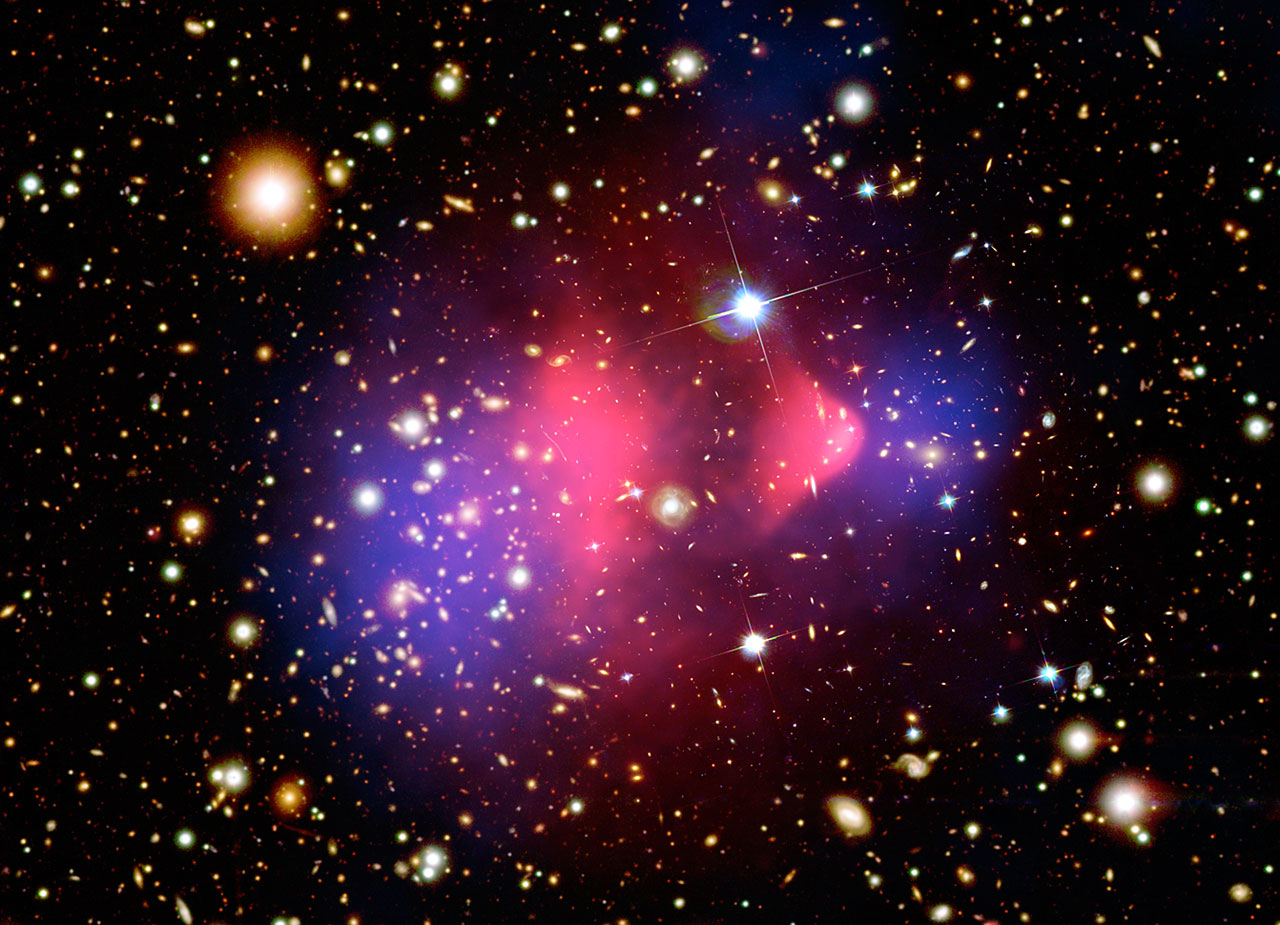
\includegraphics[width=0.85\linewidth]{revistas/002/imaxes/materiaescura2.png}
    \captionof{figure}{O Cúmulo Bala na constelación de Carina. En vermello, a emisión en raios X do gas intergaláctico; en azul, a distribución de materia escura obtida a través dos efectos de lente gravitacional \cite{hubbleNASA2}.}
\end{center}

Iso si, se ben parece estar bastante claro que a materia escura existe aínda que non a vexamos, no que respecta á súa composición a situación é moi distinta. A día de hoxe non se coñece con certeza de que está feita, mais hai moitos candidatos a materia escura. En primeiro lugar, poderíamos preguntarnos se se trata de materia ordinaria que por algunha razón resulta invisible, o cal xa está prácticamente descartado. Por exemplo, quizais sería algún obxecto compacto coma un MACHO (Massive Astrophysical Compact Halo Object), isto é, buracos negros, planetas errantes, asteroides, etc., mais os seus efectos gravitacionais serían diferentes aos da materia escura (o caso dos buracos negros primordiais aínda se está a estudar). Tampouco poden ser nubes de gas escuras (como as nebulosas escuras), pois absorberían a luz de estrelas ou galaxias distantes, o cal non observamos; a materia escura é transparente á luz. Os neutrinos descartámolos igualmente porque debido á súa ínfima masa terían velocidades moi altas e serían “quentes”, non fríos.

Algúns dos candidatos máis prometedores son os WIMPs (Weakly Interacting Massive Particle, ou partículas masivas que interactúan debilmente), dos cales o neutralino é un bo exemplo. Os neutralinos son as partículas supersimétricas máis lixeiras e posúen características interesantes compatibles coas da materia escura. Outras partículas moi estudadas son os axións, que aparecen en propostas para resolver o problema CP forte na cromodinámica cuántica. Iso si, debemos recordar que neutralinos ou axións son aínda partículas hipotéticas non detectadas experimentalmente. En realidade, para responder que é a materia escura atopamos dende partículas exóticas cuxa existencia non ten demasiado apoio teórico ou a posibilidade de que haxa dimensións extras, ata a simple ausencia de materia escura. Estas últimas teorías (chamadas MOND) suxiren unha modificación no comportamento da gravidade a grandes distancias, o cal explicaría as altas velocidades das estrelas ou galaxias xa comentadas. Non obstante, estas teorías non poderían explicar os efectos de lente gravitacional observados.

En definitiva, temos moitas probas da existencia da materia escura e coñecemos algunhas das súas características, mais o seu constituínte é incerto. Aínda que xa están descartados algúns candidatos e moitos outros probablemente descartaranse no futuro, terase que seguir investigando para resolver este enigma


\nocite{alberto2021materiaescura}
\nocite{krauss5esencia}
\nocite{hubbleNASA}
\nocite{hubbleNASA2}
\printbibliography


\end{multicols}
\end{refsection}\newpage
\Titular% 
{Donnie Darko: ciencia para estadounidenses?}%
{Emilia Prado Senlle}%
{divulgacion}%
{Breve disertación sobre a ciencia no filme \textit{Donnie Darko}.}%

\begin{refsection}
\begin{multicols}{2}


Existen moitas películas que tratan de incorporar a física nas súas tramas. O
exemplo máis notable é, probablemente, \textit{Interstellar}, coas súas viaxes
polo tempo e distintas realidades. Ademais, algo que adoitan compartir estes
filmes é a súa constante presenza en vídeos con títulos coma: <<\textit{10
películas que che farán explotar a túa mente!!!!}>> Que se viaxes no tempo, se
universos paralelos… Un lío. Claro que a confusión e a intelixencia non son
sinónimos, e o público xeral non tende a ser un bo crítico da rigurosidade
científica. Polo tanto, ao veren estes filmes que tanto xogan co espectador, a
pregunta real debería ser: é confuso porque é intelixente, ou simplemente
porque é estúpido?\\

\begin{centering}
    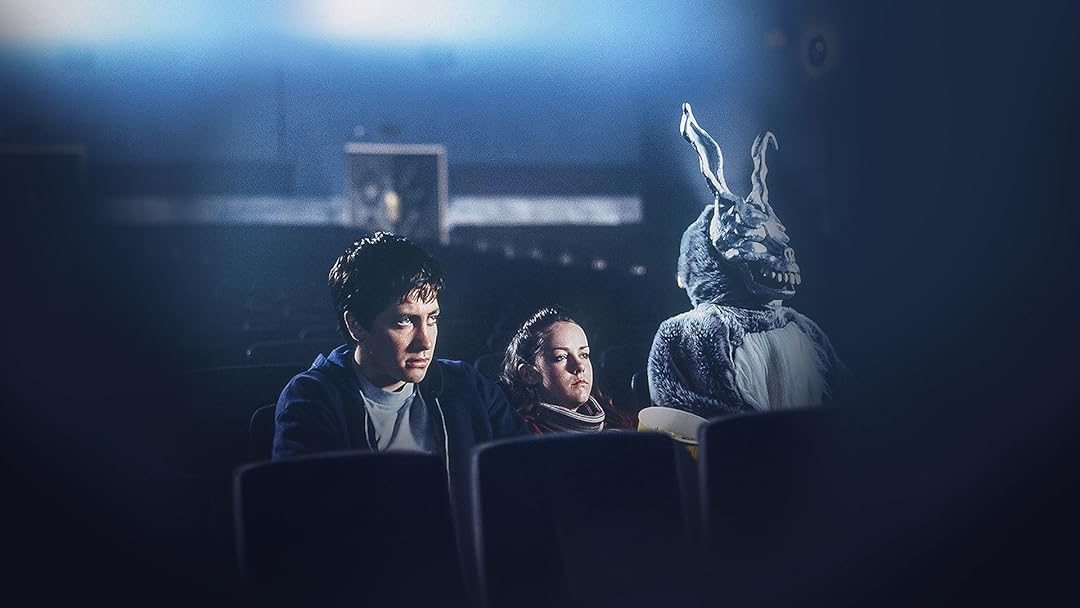
\includegraphics[width=1\linewidth]{revistas/002/imaxes/DONNIE-DARKO.jpg}
    \captionof{figure}{Fotograma, Donnie e Frank. \cite{donnie_darko}}
\end{centering}

Cando buscas Donnie Darko na Internet, a maior parte dos resultados van ser
unha versión de: <<\textit{final de \textbf{Donnie Darko} explicado con
\textbf{CIENCIA}!!!!}>>. Trátase dunha película comunmente coñecida polo seu
final confuso e a súa enrevesada cronoloxía. Foi dirixida por Richard Kelly e
rematou sendo considerada unha película de culto estadounidense tralo seu seu
lanzamento en 2001 e, máis tarde, en 2004, de \textit{Donnie Darko: The
Director’s Cut}, significativamente máis extensa ca a orixinal. A trama segue a
Donnie Darko, un adolescente que sofre de importantes problemas psicolóxicos e
comeza a alucinar cun coello xigante chamado Frank. Este coello salva a súa
vida dun accidente e avísao da inminente chegada do fin do mundo. A partir de
entón, Donnie vese obrigado a cumprir coas ordes de Frank, o que produce unha
serie de actos violentos ata o final, no que casualmente viaxa no tempo para
salvar o seu mundo da destrución.

A explicación máis común en vídeos de YouTube adoita ser unha: Donnie, ao
sobrevivir ao incidente, entrou nun universo paralelo que colapsará en pouco
tempo. Antes que iso poida ocorrer, viaxa a través do tempo ata o seu universo
de orixe, morre, e salva os seus amigos da apocalipse. Soa un pouco estúpido de
primeiras, mais o certo é que, se indagamos un pouco, podemos dar nas bases do
filme con nomes do mundo da física.

\subsection*{\textit{Donnie Darko} explicado con ciencia!}

Un concepto en que esta obra insiste moito é na de destino e determinismo, que
se presenta visualmente na forma dunha masa que se extende dende o peito de
cada ser ata o lugar onde vai estar no futuro; e aínda que semella estraño,
este é un concepto físico existente, aínda que algo reinterpretado. Os físicos
David Deutsch e Michael Lockwood explican que a vida forma unha especie de
``verme’' de 4 dimensións, cunha cola que representa a orixe da vida, e unha
cabeza na que se atopa a morte \cite{deutsch.m_1994}. Así, un obxecto como
o vemos no presente non é máis que a intersección nun espazo tridimensional
entre este e o seu ``verme'’.  Por suposto, a película céntrase máis no aspecto
filosófico desta cuestión; se podemos ver o futuro, significa que é inevitable?
Existe o destino? Está xa decidido que vou ser un fracasado? O cal é unha
pregunta moi interesante, e moi explorada dende tempos do determinismo
mecanicista do Renacemento ata a actualidade. Con todo, esta cuestión
científica e filosófica vese rapidamente destruída polo propio guión. Donnie,
en resposta ás dúbidas filosóficas do seu profesor de ciencias, di: <<non [está
decidido] se quedas na Canle de Deus>>\cite{donnie_darko}.
Así, fácil. Deus.\\

Podería opinarse que este intento por explicar o físico mediante o místico, ou
de incluír a Deus dunha forma tan repentina e fóra de lugar no argumento,
pódese ignorar un pouco ao ter en conta que o filme supón, en grande medida,
unha crítica á mentalidade cerrada e tradicionalmente relixiosa dos suburbios
americanos. Ademais, ao recurrir á versión de corte do director da película,
ofrécesenos unha explicación sobre o universo de Donnie moito máis completa ao
incluír extractos do libro de Roberta Sparrow, outra personaxe da película.
Este leva o nome de \textit{A Filosofía das Viaxes no Tempo}, e fala sobre a
formación de Universos Tanxentes extremadamente inestables a partir de
incidentes no Universo Primario. Iso explicaría todo o tema da fin do mundo,
pero… realmente ten sentido?

É obvio que os universos paralelos ou múltiples non son un tema inexplorado
pola física moderna. Por exemplo, para explicar a `superposición’ das
partículas subatómicas en múltiples estados instantáneos, Hugh Everett refírese
ao que posteriormente se bautizou como a \textit{Interpretación de Mundos
Múltiples}. Esta describe que cada un dos estados nos que atopamos unha
partícula ocorren simultaneamente, só que en distintas ramas do universo e cada
vez que tratamos de observala, o universo divídese en distintas realidades
paralelas \cite{gribbin2004historia}. É claro que esta non é unha tese demasiado
consolidada no mundo científico, xa que non hai forma de demostrala
experimentalmente. Pero existe e é obvio que Donnie Darko bebe destas ideas;
nun universo, Donnie está vivo, e noutro, morto.

Pois, entón, estas realidades non deberían interactuar de ningunha forma, non
si? Como pode ser que Donnie volva ao seu universo orixinal ao final da
película? Ou que Frank, que é en realidade o amigo morto de Donnie, volva atrás
no tempo para avisar da fin do mundo? Pois ben, a película realmente non o
explica. O libro de Roberta Sparrow menciona as viaxes no tempo, mais cunha
explicación vaga e demasiado mística para ser científica, <<\textit{A Auga e o
Metal son os elementos chave para as Viaxes no Tempo. A Auga é o elemento
barreira para a construción de Portais de Tempo que conectan Universos no
Vórtice Tanxente}>> \cite{donnie_darko}.\\

Con todo, na física, existe quen tratou estes problemas. Por exemplo, Kurt
Gödel e a súa métrica de Gödel, coa que pretendeu solucionar as ecuacións de
campo de Einstein. Esta presenta a existencia de cadeas causais pechadas, nas
que o evento orixinal se causa a si mesmo \cite{nunez.r_2021}. Claro que esta é unha
teoría que se cuestiona profundamente como verdadeira (véxase o paradoxo do
avó). Aínda así, é algo interesante de explorar; a pesar de que a película nin
tan sequera trate de facelo, máis aló de referirse a unha viaxe no tempo
inexplicable, a partir dun buraco no espazo-tempo inexplicable, e cunhas
consecuencias… dubidosas. É obvio que así vai quedar un final, como mínimo,
confuso.

\subsection*{Cine e... ciencia?}

Por suposto, isto non significa que unha película deba ofrecer unha explicación
pormenorizada, argumentada e cun sentido científico riguroso. Ao final, é
ficción, e perdería un pouco a graza se houbese que incluír unha bibliografía
citada en Harvard ao final dos créditos. E o certo é que a trama ten as súas
bases, ata certo punto. Con todo, resulta dubidoso cando unha obra trata de
parecer profundamente complexa e intelixente cando non é máis que uns cantos
conceptos físicos empregados ao servizo do guión; e cando a conversación máis
científica que podemos escoitar nela é a explicación dun profesor de instituto
sobre o que son os vectores no espazo. Ao final do día, tampouco se pode culpar
disto a un filme tan claramente feito para o público estadounidense xeral.

\nocite{deutsch.m_1994}
\nocite{donnie_darko}
\nocite{gribbin.j_2020}
\nocite{nunez.r_2021}
\nocite{wisecrack_2019}

\printbibliography

\end{multicols}
\end{refsection}
\newpage
\Titular%
{O efecto Dzhanibekov}%
{Martín Alberto Häderli Revuelta}%
{divulgacion}%
{Un fenómeno físico que conecta aos mongois, Euler e... a fin do Mundo?}%

\begin{refsection}
\begin{multicols}{2}


É o turno de adentrarse nunha das conexións máis curiosas da física: como
poderían conectarse o Imperio mongol, a fin da carreira espacial entre a URSS e
os EUA, a apocalipse e, como non, Euler? Prepárate, porque quizais terminamos
dando... algunha que outra volta; imos, pois, falar do \textit{\textbf{Efecto
Dzhanibekov}}.

\subsection*{A historia}

O punto de partida da nosa aventura é o 11 de febreiro de 1985, no medio da que
é popularmente recoñecida como a etapa máis tensa da Guerra Fría. Os sistemas
de control da estación espacial soviética Salyut 7 fallaron e perdeuse o
contacto coa nave. Ao non haber tripulantes nese momento, a estación espacial
comezou a vagar sen control, rotando sobre o seu eixo axial, que é o eixo
principal con menor momento de inercia. Isto foi crucial, dado que segundo a
dinámica do corpo ríxido o movemento dun corpo que xira sobre un dos seus eixos
principais é estable sempre e cando teñan asociados ou o menor ou o maior
momento de inercia (recordaremos isto máis adiante). Consecuentemente, aínda
existía unha pequena posibilidade de iniciar unha misión espacial para tentar
reparar os fallos e recuperar o control sobre a Salyut 7. Porén, era necesario
recrutar os cosmonautas adecuados e aí é onde entra en escena o noso
protagonista: \textbf{Vladimir Aleksandrovich Krysin}.\\

\begin{centering}
    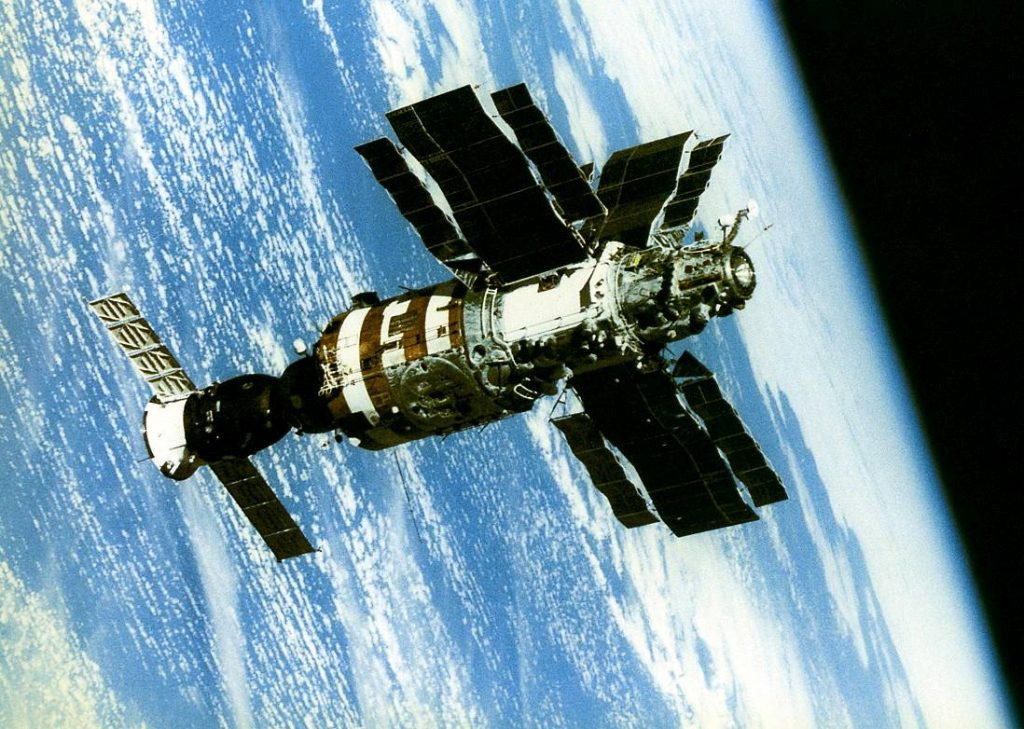
\includegraphics[width=0.8\linewidth]{revistas/002/imaxes/img1.jpg}
    \captionof{figure}{Estación espacial Salyut 7.}
    \label{fig:salyut}
\end{centering}\vspace{10pt}

Vladimir naceu no actual Uzbekistán e estudou física na Universidade de
Leningrado para posteriormente graduarse como instructor de voo nas Forzas
Aéreas Soviéticas, onde logo foi seleccionado como cosmonauta. Á idade de 22
anos casou con Liliya Dzhanibekova, descendente directa de Janibeg, un líder
medieval dun dos reinos que quedaron logo da disolución do Imperio Mongol. Como
consecuencia de que o pai de Liliya non tiña fillos varóns, Vladimir decidiu
adquirir o apelido da súa muller como forma de honrar aos seus ancestros e
continuar coa liña de descendencia, pasando a chamarse \textbf{Vladimir
Dzhanibekov}. Durante os seguintes anos, Dzhanibekov participou en cinco
misións espaciais, e foi nesta última onde descubriu o efecto que toma o seu
apelido, mais non nos adiantemos.

Regresemos ata o 6 de xuño de 1985 no cosmódromo de Baikonur, actual
Kazakhstán. Ás 06:39:52 dese mesmo día despegou de alí a nave Soyuz-U2, a bordo
con Dzhanibekov e un enxeñeiro de voo co fin de recuperar a Salyut 7. Dado o
feito de que o xiro da estación era estable, os soviéticos puideron facer as
manobras para se aproximaren o suficiente á nave e facer coincidir as rotacións
conseguindo finalmente recuperar o control da estación espacial, así
converténdose esta nunha das fazañas máis notables da astronáutica. Unha vez
comprobaron que o aire era respirable, os cosmonautas entraron na estación e
comezaron a facer as reparacións necesarias. Dezanove días despois, ocorrería o
achado. Mentres Dzhanibekov desempacaba a subministración do envío espacial
Progress-24, unha porca con dúas ás saíu xirando do seu sitio. O problema viu
cando logo duns segundos, este elemento cambiou de orientación e puxérase a
xirar noutro sentido como se de maxia negra se tratase. O cambio de orientación
na rotación dun obxecto que en principio non estaba a xirar nese eixo é o que
actualmente se denomina como \textbf{efecto Dzhanibekov} ou tamén
\textbf{teorema da raqueta de tenis}.\\

\begin{centering}
    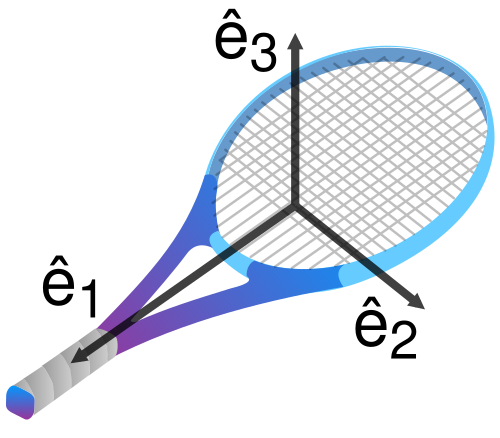
\includegraphics[width=0.6\linewidth]{revistas/002/imaxes/Tennis_racquet.png}
    \captionof{figure}{Eixos principais dunha raqueta de tenis.}
    \label{fig:raqueta}
\end{centering}\vspace{10pt}

No noso día a día podémolo visualizar facilmente, por exemplo, se colles o teu
tubo de pasta de dentes, o agarras dende o lado oposto á tapa (co logo cara
arriba) e o lanzas sobre sí mesmo, se tes a maña necesaria (moita) para volvelo
agarrar, verás que agora está boca abaixo. Este fenómeno é moito máis visible
nas raquetas de tenis, de aí o seu nome. Un posible efecto secundario é que o
coñecedor do fenómeno vai pasarse unha semana lanzando obxectos co fin de
comprobalo, e co fin de evitalo, imos tentar explicar a física do asunto.


\subsection*{A física do fenómeno: Por que?}

Co obxectivo de explicar o porque deste fenómeno temos que desempolvar os nosos
apuntamentos de Mecánica Clásica II e recordar que o movemento xiratorio dun
obxecto (sólido ríxido en términos físicos) depende principalmente da dirección
en que xiremos o corpo e o ``esforzo'' que supón manter a rotación neste eixo.
É dicir, custa menos enerxeticamente xirar un cilindro sobre o seu eixe axial
que se o xiramos sobre un eixe perpendicular a este coa mesma velocidade
angular. As ferramentas matemáticas que nos dan esta información son o vector
de velocidade angular ($\vec{\omega}$) e o tensor de inercia ($\mathbb{I}$).
Pero aínda queda a parte máis importante: obter o movemento do obxecto (as
ecuacións do movemento), que se conseguen unha vez se resolvan as ecuacións de
Euler que relacionan as compoñentes da velocidade angular e do tensor de
inercia (tamén chamados momentos de inercia) nun determinado sistema de
referencia. Como estamos a traballar nun espazo de 3 dimensións, as compoñentes
da velocidade angular e momentos de inercia tamén serán 3, por simplicidade:
$\omega_1, \omega_2, \omega_3$ e $I_1, I_2, I_3$.\\

En principio, este sistema de ecuacións diferenciais pode ser sinxelo de
resolver se o obxecto é moi simétrico, pero este non é o caso da porca ou da
raqueta de tenis, polo que temos que esforzarnos máis para obter información
destes movementos. Como xa adiantamos anteriormente, se consideramos un xiro
maioritario nun dos eixos principais e xiros minoritarios nos outros eixos,
chegamos a que as ecuacións de Euler nos din que o movemento naquel eixo
principal asociado ao momento de inercia intermedio ($I_1>I_2>I_3$, por
exemplo) é inestable, feito que explica a aparición do efecto Dzhanibekov.
\textit{Pero entón non temos unha solución analítica para o movemento?} Si
existen, o problema é que involucran ferramentas matemáticas máis profundas,
como as funcións elípticas de Jacobi \cite{RouthDynamics} ou o elipsoide de
Poinsot \cite{VanDamme2017}, polo que non imos entrar en detalles.

\subsection*{Aplicacións e consecuencias: Apocalipse?}

Unha das razóns polas que o goberno soviético ocultou este fenómeno foi
principalmente polo medo a que a Terra, ao ser un corpo que non é perfectamente
simétrico, puidese sufrir este mesmo efecto, o que, evidentemente, sería
catastrófico. Non obstante, a masa da Terra está disposta tal que xira sobre o
seu eixo de menor inercia e polo tanto, de forma estable, evitando a
apocalipse. Igual que coa Terra, ocorre o mesmo cos demais planetas, polo que é
xusto preguntarnos por que os planetas xiran sobre o seu eixo de menor inercia
e isto é consecuencia directa da conservación do momento angular herdado do
disco protoplanetario que formou o Sistema Solar. Aínda así, detectáronse unha
serie de lúas orbitando aos planetas gaseosos que si amosan este efecto e, máis
interesante aínda, publicouse recentemente que unha variedade de púlsar chamado
magnetar tamén pode sufrir este mesmo efecto por culpa do seu campo magnético
extremo e provocar ondas gravitacionais \cite{Kantor2023}. Finalmente, tamén se
teorizou coa posibilidade de empregar este efecto para a construción de naves
que aproveiten o fenómeno para cambiar o sentido da viaxe, o que reduciría
considerablemente o peso e o combustible necesario para estas misións
\cite{Ono2022}.

\printbibliography

\end{multicols}
\end{refsection}
\newpage
\Titular%
{Memorias de Moscova}%
{Carlos Merino}%
{divulgacion}%
{Dpto. Física de Partículas - Facultade de Física, IGFAE\\
Universidade de Santiago de Compostela}%

\begin{refsection}
\begin{multicols}{2}

\subsection*{En homenaxe a Alexei B. Kaidalov}
%\subsection*{\small Compostela, 4 de maio de 2025}

O estudo da Física Hadrónica e da interacción forte responsable de manter aos nucleóns (protóns e neutróns) dentro do núcleo atómico e aos quarks (as partículas fundamentais que sinten esta interacción) confinados nos hadróns ten sido unha das líneas de investigación máis importantes na Física dende o fin da da Segunda Guerra Mundial e durante estas primeiras décadas do século XXI. Os avances asombrosos neste campo débense tanto ao traballo teórico máis fundamental e punteiro, como aos fitos experimentais acadados polas grandes colaboracións experimentais internacionais que en laboratorios como o Centre Européen pour la Recherche Nucléaire (CERN), de Xenebra (Suíza), desafían cada día os límites tecnolóxicos e de obtención e análise de datos. Esperamos nos conduzan a novos horizontes e retos científicos, entre eles o da obtención sistemática e completa descripción dun novo estado da materia, o plasma de quarks e gluóns (QGP), unha fase na que os quarks e gluóns están deconfinados, e que recupera o estado da materia no universo instantes despois do Big-Bang e antes da formación da materia hadrónica.

O grupo de Fenomenoloxía do Departamento de Física de Partículas e do Instituto de Física de Altas Enerxías (IGFAE) da Universidade de Santiago de Compostela leva traballando moitos anos no desenvolvemento de modelos fenomenolóxicos que permitan avanzar na predición e descrición dos datos experimentais dende a perspectiva teórica da Cromodinámica Cuántica (QCD). Esta é a teoría cuántica de campos basada no grupo de Lie non-abeliano $SU(3)$, que describe a interacción forte no Modelo Standard no que se codifica o coñecemento certo que, hoxe en día, co consenso da comunidade científica, e ratificado polo experimento, temos da realidade física e material do Universo.

En moitas ocasións, este labor de investigación das/os físicas/os do grupo de Santiago de Compostela tense levado, e segue a levarse a cabo agora mesmo, en colaboración con facultades, laboratorios e centros de investigación punteiros de moitos outros países como Alemaña, Armenia, China, Estados Unidos de América, Francia, Portugal, Ucraína, etc.

Neste senso, unha colaboración especialmente frutífera ten sido a desenvolta con grupos da antiga Unión Soviética, berce dunha das grande escolas e tradicións da Física do século XX, apoiada en algunhas das figuras máis insignes da historia da Física, como Lev Davidovich Landau, que tiveron que levar adiante o seu labor de investigación e maxisterio nunhas circunstancias vitais marcadas por uns tempos difíciles e moitas veces tráxicos.

Unha figura capital na Física Hadrónica desta escola rusa foi Alexei Borisovich Kaidalov (1940-2010), do Intituto de Física Teórica e Experimental (ITEP), de Moscova. Coñecín persoalmente a Alexei Kaidalov durante os últimos anos da década dos 80 do século pasado, durante a preparación da miña tese de doutoramento baixo a dirección de Alfóns Capella (o Profesor Carlos Pajares era codirector da tese na USC), no Laboratoire de Physique Théorique  et des Hautes Énergies (LPTHE) da Université de Paris-Sud, Paris XI, en Francia, onde Alexei realizaba unha estadía de investigación para traballar con Alfóns e con Jean Tran Than Van. Lembro que dende o primeiro momento Alexei me causou unha grande impresión, que se viu reforzada pola paciencia e o tempo que investiu en discutir de Física co xoven estudante de doutoramento que era eu nese momento.

\begin{center}
    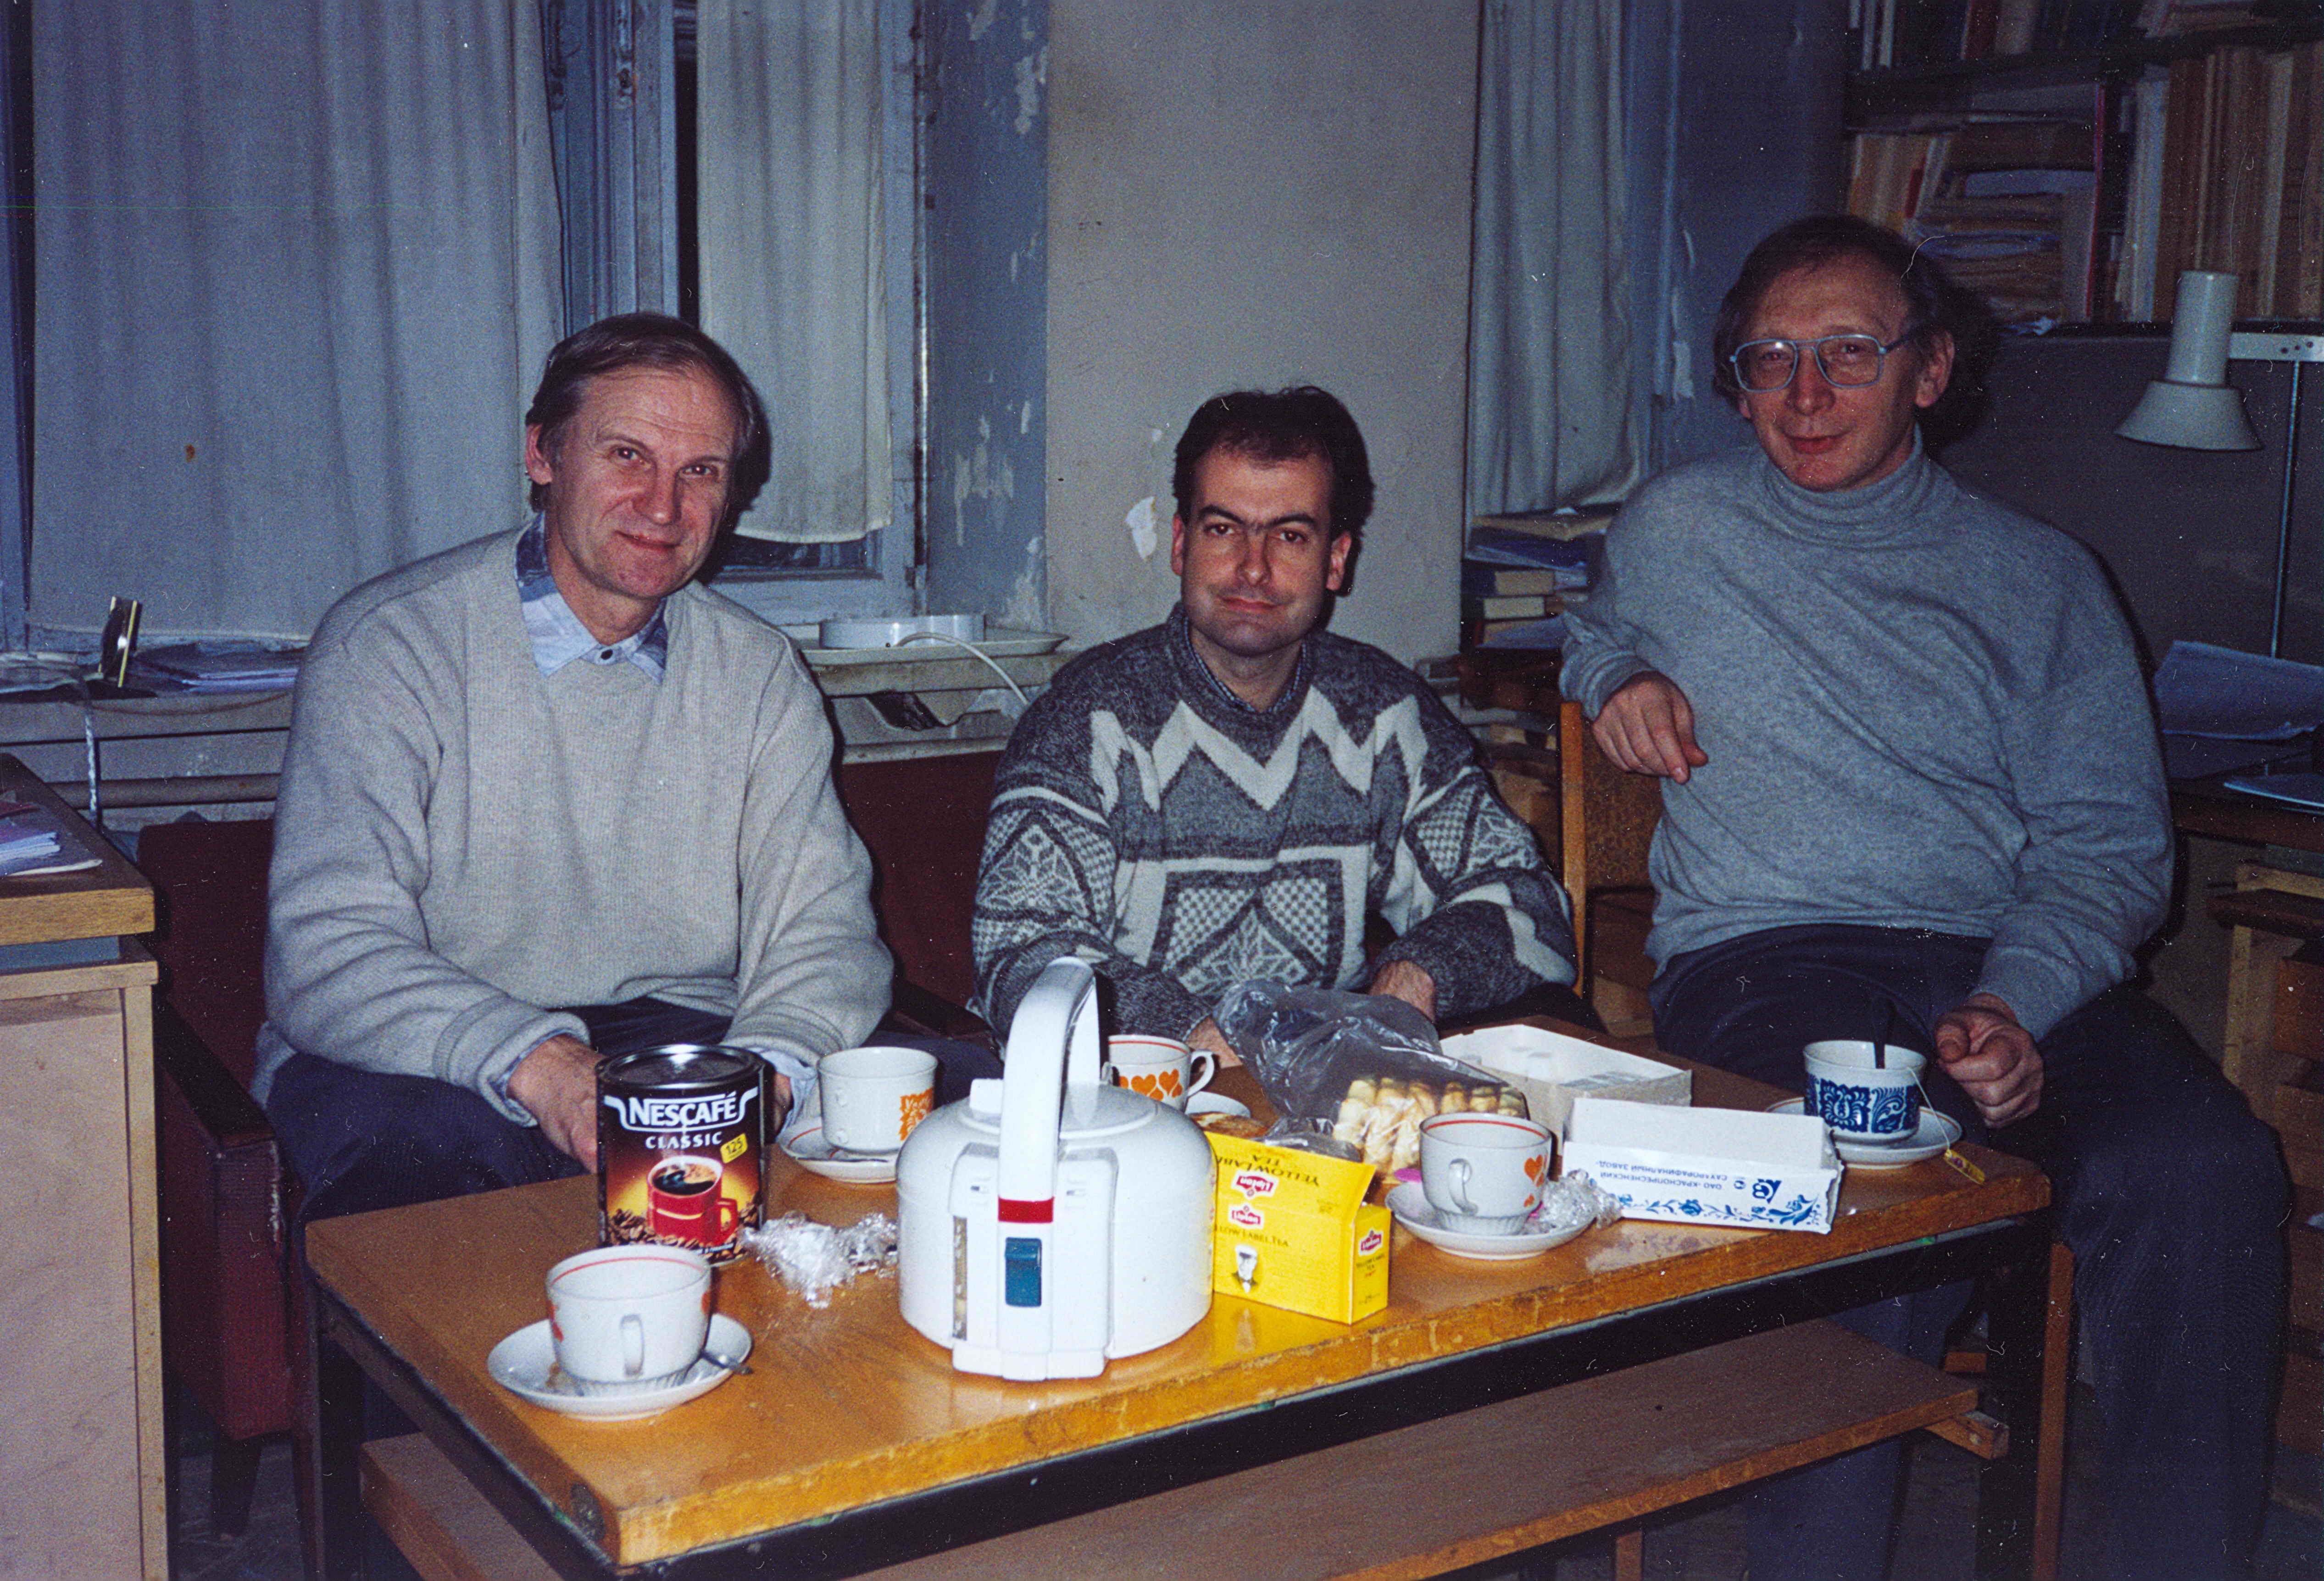
\includegraphics[width=0.9\linewidth]{revistas/002/imaxes/Kaidalov_Picture.jpg}
    \captionof{figure}{Alexei B. Kaidalov, Carlos Merino e Konstantin G. Boreskov durante unha pausa para o café/té no ITEP de Moscova (Rusia), nalgún momento en xaneiro-febreiro de 1993 (foto do arquivo de Carlos Merino).}
\end{center}    

Algún tempo despois da defensa da miña tese de doutoramento, Alexei veu a Compostela para participar, xunto con Konstantin G. Boreskov e o grande Karen A. Ter-Martirosian (alumno de Landau, e mestre de Alexei, pero tamén de Gribov, Polyakov, Migdal, Zamolodchikov, e tantos outros), no XXII International Symposium on Multiparticle Dynamics, organizado polo Profesor Carlos Pajares. O feito de que físicos con tanta sona e dunha institución tan prestixiosa como o ITEP estiveran na nosa Facultade resultou moi inspirador nese momento para as/os novas/os doutoras/es que estábamos a comenzas as nosas carreiras científicas. Durante a conferencia, Alexei e Konstantin invitáronme a visitar  ITEP, onde pasei un mes en xaneiro-febreiro de 1993. Ademáis da extraordinaria experiencia de estar nqueles tempos nunha institución tan importante na historia da física teórica durante o século XX, e de poder apreciar de primeira man o legado de figuras extraordinarias como Isaak Yakovlevich Pomeranchuk (do que recibe o seu nome o Pomerón, a traxectoria de Regge cos números cuánticos do baleiro que explica o aumento da sección eficaz hadrónica coa enerxía), do que Alexei foi o último alumno de doutoramento, puiden gozar dunha introdución entrañable á cultura rusa, e das invitacións a compartir vodka e sakuska (os entrantes fríos que se serven como parte da comida imprescindible para acompañar a inxesta de vodka).

Vodka é o diminutivo da palabra rusa voda, que significa auga. O vodka foi durante moito tempo un piar económico fundamental do sistema zarista, pero a finais do século XIX a producción masiva sen ningún control, nin no procedemento nin nos ingredientes, dou lugar a unha crise de falecementos, casos de ceguera, etc. que decidiu ao Zar a tomar medidas, aínda coa perda que esto podía causar ás finanzas do estado e da casa imperial. Como consecuencia desta decisión, se lle encargou a Dmitri Ivánovich Mendeléyev que atopara un método para fixar a producción reglada e evitar a proliferación de vodkas nocivos para a saúde. Mendeléyev descubriu que se se lle prendía lume a estas bebidas alcohólicas destiladas, estas ardían por enriba dos 40º de alcohol, e estableceu este criterio para definir o vodka legal, que dende ese momemto non pode ter unha concentración máis grande de alcohol. A partir dese momemto, os funcionarios do estado visitaban as granxas e as destilerías nas que se producían a bebida destilada, e simplemente lle prendían lume: se a concentración de alcohol era superior aos 40º o líquido ardía e o destilador perdía o que producira. O que non ardía era o que despois a xente podía beber, pero afeitos a concentracións de alcohol moito máis grandes, ao catalo o bebedor os rusos reaccionaban decindo vodka! (auguiña!). Sexa como for, a inmensa maioría dos rusos concordan en que a Táboa Periódica foi a segunda contribución máis importante de Mendeléyev á Humanidade (a primeira, foi, sen dúbida, o vodka).

Nunha desas ocasións nas que fun invitado a unha reunión no apartamento dun dos membros do ITEP para falar, beber vodka e comer sakuska, recordo que cando chegábamos ao lugar do encontro a media tarde, despois de saír do laboratorio, e Konstantin G. Boreskov e eu facíamos os últimos metros a pé, a temperatura era moi baixa (varios graos por debaixo de cero graos celsius), e a sensación térmica era de moito frío. Despois, ao cabo de varias horas, xa de noite arredor da medianoite, ao saírmos do edificio para coller o último metro de volta a Profsoiuznaia (Unións Profesionais-Sindicatos), a estación no suroeste do Moscova máis cercana á residencia na que me aloxaba, aínda que a temperatura era moito máis baixa, e o aire era glacial, tiven a impresión de non sentir tanto frío como á chegada, e comenteillo a Boreskov, que cun sorriso na boca, e alzando o dedo índice da man dereita cuberta pola luva, díxome: "Querido Carlos, agora xa entendes por que os rusos bebemos vodka!".

Máis tarde, a principios de 1994, cando eu estaba a realizar un postdoc no LPTHE, Alexei veu pasar uns meses no laboratorio. A súa presenza tivo un impacto inmediato na actividade investigadora do grupo dirixido por Alfóns Capella, o que se traduciu na publicación de varios papeis adicados á descripción da física de baixo-$x$ e publicados en revistas internacionais de primeiro nivel, e dos que tiven o privilexio de ser co-autor.

Nestes anos en París, que Alexei visitou máis veces, e durante moitos anos despois, coincidín con Alexei en moitas conferencias e meetings, en particular en Les Reancontres de Moriond, organizados cada mes de marzo por Jean Tran Than Van nos Alpes, ben en Les Arcs ou Méribel (Francia), ben en La Thuile (Italia), e onde as fazañas no esquí de Alexei case igualaban a brillantez das súas charlas de Física. Sempre me admirou como Alexei era quen, despois de adicar as tardes a esquiar, e de pasar moitas horas a discutir coas/os participantes teóricos e experimentais na conferencia que viñan pedirlle a súa opinión e o seu consello sobre os problemas máis diversos nos que estaban a traballar, de preparar unha charla final tan precisa e completa, que proporcionaba unha imaxe clara e total da actividade e dos resultados científicos presentados durante a conferencia, e das súas perspectivas de futuro. É ben coñecida a anécdota de cando no instante despois de finalizar e enviar para a súa publicación, con outros colegas, un papel moi importante que tiña requerido un esforzo moi grande, mentres os outros colegas respiraban relaxados, Alexei, sen solución de continuidade, simplemente se dirixiu ao seu escritorio, colleu (antes da existencioa dos ordeadores personais) papel e lápis , e empezou a escribr, impasible, o seguinte artigo, que tiña xa redactado de principio a fin na súa cabeza.

Colaborei con Alexei durante case vinte anos, en funcións de estructura, disociación difractiva, diffracción hard, producción de barións estraños, funcións de estructura nuclear, etc, e somos co-autores dunha decena de papeis, pero son plenamente consciente de que esta bagaxe representa unha parte mínima do labor titánico e dos logros fundamentais que Alexei Kaidalov ten aportado á Física de Partículas. Posiblemente Alexei foi o maior experto mundial en difracción, e unha lista moi breve das súas contribución máis importantes podería ser a seguinte: 1. A consideración das desintegracións non-leptónicas e radiactivas de hiperóns; 2. A identificación das sinaturas dos cortes running de reggeóns nos datos experimentais; 3. A reformulación do modelo de intercambio de un pion no marco do enfoque reggeónico, e as consecuencias cuantitativas na descrición dunha grande cantidade de datos experimentais; 4. A análise dos procesos de disociación difractiva a altas enerxías; 5. O desenvolvemento das regras de suma para a dispersión reggeón-hadrón, que permite predecir algunhas resonancias de espín elevado; 6. A formulación do Modelo de Cordas Quark-Gluón (QGSM) para a multiprodución a enerxías altas e moi altas, que permitiu a descrición cuantitativa dunha grande cantidade de datos experimentais en colisións hadrón-hadrón, hadrón-nucleo, e núcleo-núcleo; 7. A descrición da produción de partículas en colisións de ións pesados, e dos efectos de apantallamento nuclear inelástico; 8.A análise dos quarks pesados a da produción de pares de leptóns en colisións sobre albos nucleónicos e nucleares.

Ao longo da súa extraordinaria carreira Alexei Kaidalov foi autor e co-autor de máis de trescentos artigos científicos publicados, dos que máis de vinte teñen cen ou máis citas, mantivo colaboracións con moitos grupos doutros países, e foi membro da colaboración experimetal ALICE, do CERN. As/os profesoras/es Néstor Armesto, Elena González Ferreiro e Carlos A. Salgado, do Departamento de Física de Partículas da Facultade de Física e do IGFAE da USC, traballaron tamén con Alexei Kaidalov, e son co-áutoras/es con el de artigos publicados en revistas especializadas.

Alexei Kaidalov foi un mestre respectado e admirado por colegas e amigos de todo o mundo, primeiro
polas súas moitas e moi importantes, a miudo fundacionais, orixinais achegas ao campo da Física de Partículas, pero tamén en especial pola súa grande xenerosidade ao transmitir ás novas xeracións de físicas e físicos, a través de explicacións claras, intuitivas e rigurosas, o seu profundo coñecemento dos principios e regras que rixen os procesos físicos. Ademáis da súa adicación en corpo e alma á Física, Alexei foi unha persoa optimista (maravilloso cantante do repertorio populas ruso), de mente cultivada e aberta, que valoraba moito a familia e a amizade, e que estaba moi orgulloso do seu país e da súa cultura\footnote[1]{Curiosamente, cando no ano 2013, os organizadores do 1st International Kaidalov Workshop on the Phenomenology of High Energy Particle Physics, adicado a memoria de Alexei, me pediron que escribira unha semblanza [1] (en inglés) sobre el, os amigos e colegas rusos que leron o manuscrito antes da súa publicación pedíronme que non utilizara o termo cosmopolitan, que nas demáis linguas ten unha connotación positiva e eu empregaba como un eloxio, porque en ruso, e dende os primeiros anos da Revolución Bolchevique, kosmopolitichnyy ten o sentido negativo de axente extranxeiro, persoa decadente, ou traidor.}.

Colaborar con Alexei Borisovich Kaidalov ten significado para min o poder aproximarme á excelencia na Física, e a apreciar un exemplo de ética no traballo e de integridade na vida, que nos debe guiar na seriedade e xenerosidade cara aos demáis no noso labor académico e de investigación, e que, ademáis, nos debe reafirmar no convencemento da valía das/os graduadas/os na Facultade de Física da USC para, a través do traballo persoal, colaborar activamente de xeito positivo coas físicas e físicos de calquera outra universidade ou centro de investigación do mundo.

\subsection*{Agradecementos}

O autor quere felicitar aos membros da DAF polo seu traballo a prol da vida e actividade da Facultade, e pola súa iniciativa de recuperar a revista da Facultade, plataforma na que compartir experiencias e inquedanzas, alumnas/os, profesoras/es e persoal de administración e servizos, que desexo se vexa refrendada polo éxito. Agradezo a Sebastián Táboas e a todo o Comité Editorial da revista, a súa invitación a contribuír con este artigo neste segundo número, e a súa paciencia á hora de ser indulxentes co prazo de entrega do mesmo, e a Belén Merino a súa revisión do texto. Espero que este segundo número de MOMENTUM teña continuación en moitos máis números no futuro. 

\nocite{Merino_2015}

\printbibliography

\end{multicols}
\end{refsection}\newpage
\Titular*%
{Viaxeiros espaciais. Oda á Voyager 1}%
{Celia Álvarez Álvarez}%
{historia}%
{De como a Voyager 1 partiu dende a Terra ata o espazo profundo.}%

\begin{refsection}
\begin{multicols}{2}

\subsection*{\textit{Na beira do océano cósmico}.}

<<\textit{A superficie da Terra é a beira do océano cósmico. Dela aprendemos a
maior parte do que sabemos. Recentemente metémonos un pouco no mar, vadeando o
xusto para mollarnos os dedos dos pés ou, como moito, para que a auga nos
chegase aos nocellos. A auga parece convidarnos a continuar. O océano chámanos.
Hai unha parte de nós que sabe que vimos de alí. Desexamos volver. Non creo que
estas aspiracións sexan irreverentes, mesmo se poden desagradar aos deuses,
sexan cales foren os posibles deuses.}>> 

%\vspace*{-1mm}
%\begin{flushright}
%Carl Sagan, \textit{Cosmos} (adaptación).
%\end{flushright}
\hfill Carl Sagan, \textit{Cosmos} (adaptación). \\

A misión de investigación espacial Voyager, fundada pola NASA, está constituída
por dúas sondas interestelares irmás: a Voyager 1 e a Voyager 2.

Durante a travesía do Voyager 1 tiveron lugar investigacións exploratorias dos
sistemas planetarios xoviano e saturniano e do medio interplanetario. O estudo
abrangueu a mellora na nosa comprensión das dinámicas atmosféricas de Xúpiter e
Saturno, dos seus campos gravitatorios, das súas magnetosferas, das
interaccións dos satélites con todos estes factores, das composicións
atmosféricas e superficiais de satélites como Titán ou os catro satélites
galileanos: Io, Europa, Ganímedes e Calisto, da Gran Mancha Vermella de Xúpiter
ou dos aneis de Saturno.

Para iso, a Voyager 1 levou a bordo instrumentos para desenvolver once
investigacións científicas, entre elas: o \textit{Imaging Science System}
(ISS), que permitiu capturar espectaculares imaxes do sistema solar; o
\textit{Infrared interferometer spectrometer and radiometer} (IRIS), que
permitiu obter perfís de enerxías e temperaturas; o \textit{Triaxial Fluxgate
Magnetometer} (MAG), que investiga os campos magnéticos de planetas e do espazo
interplanetario; o \textit{Low Energy Charged Particle Instrument} (LECP), que
mide propiedades de electróns ou ións de plasma detectados; ou o \textit{Plasma
Wave Subsystem} (PWS), que tamén se utiliza no estudo de magnetosferas e da
interacción local onda-partícula. Actualmente só o MAG, o LECP e o PWS se
atopan activos.

A sonda obtén a súa enerxía de tres xeradores termoeléctricos de radioisótopos,
que funcionan grazas á desintegración do óxido de plutonio. Estes xeradores
converten calor producido na desintegración radioactiva en enerxía eléctrica. A
potencia dos xeradores diminúe co tempo debido á semivida do combustible e á
degradación dos termopares, polos cales se converte enerxía térmica en
eléctrica mediante o efecto Seebeck. Durante a navegación utilízanse sinais do
rastreador solar e estelar para conservar a antena de radio do Voyager
orientada cara á Terra activando pequenos propulsores do sistema de propulsión
da Voyager.

\subsection*{Viaxe. Navegando polo sistema solar.}

Dúas naves Voyager ían ser lanzadas durante a ventá % igual hai que darlle
voltas a esa expresión dun mes que comezaba a finais de agosto de 1977,
coincidindo cun aliñamento especial  dos planetas exteriores que permitiría o
uso dos seus campos gravitacionais para cambiar a velocidade e dirección da
sonda e así facilitar a súa viaxe dun cara ao seguinte.

Orixinalmente programada para partir doce días despois da Voyager 2, a Voyager
1 tivo o seu despegue a bordo do vehículo de lanzamento \textit{Titan IIE} tras
ser aprazado en dúas ocasións para previr os problemas que sucederan tralo
lanzamento da Voyager 2. A partida definitiva da sonda sucedeu o 5 de setembro
de 1977 ás 12:56:00 UTC dende a Estación da Forza Espacial de Cabo Cañaveral
(Florida, EEUU), cun lanzamento impecable e preciso. O 6 de setembro, un día
despois da partida, a Voyager despediuse da Terra e da Lúa mandando a súa
primeira foto do noso hogar e o seu único satélite.

Pouco despois da saída da Voyager da órbita terreste todos os instrumentos
científicos acendérose para aproveitar as características que se comparten a
Terra e a Lúa con Xúpiter, Saturno e os seus satélites; realizáronse
observacións útiles para a súa calibración. Trinta días despois do lanzamento
comeza oficialmente a fase de cruceiro ata o encontro con Xúpiter. Os
instrumentos para o estudo de campos e partículas na Voyager investigaron
durante este tempo a rexión interplanetaria Terra-Xúpiter. A Voyager 1 adiantou
á Voyager 2 tras adentrarse no cinto de asteroides.

Ointenta días antes do encontro con Xúpiter comezaron as observacións do
planeta e dos satélites galileanos. A esta distancia a cámara ISS da Voyager
pode obter unha resolución comparable ou mellor que a alcanzable na Terra. A
Voyager 1 alcanza o seu achegamento máis próximo a Xúpiter o 5 de marzo de
1979: a sonda sobrevoou o satélite xoviano Amaltea, descubrindo a súa forma
alongada; seis horas despois, a Voyager atoparase a uns 350.000 km do centro de
masa de Xúpiter para logo sobrevoar Io, Europa, Ganímedes e Calisto.

\begin{center}
    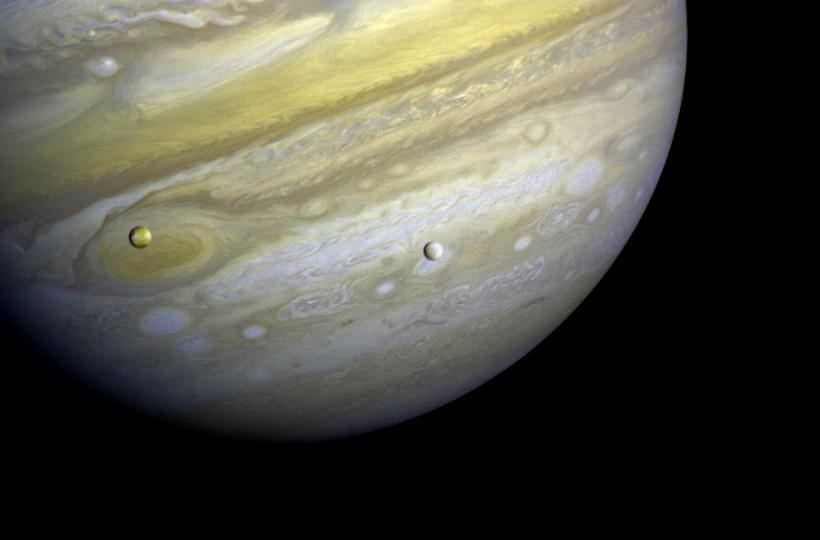
\includegraphics[width=0.9\linewidth]{revistas/002/imaxes/jupiter.jpg}
    \captionof{figure}{Xúpiter cos satélites Io (esquerda) e Europa.}
\end{center}

Descubríronse o sistema xoviano de aneis e dúas lúas, Thebe e Metis, detectouse
o primeiro relámpago nun mundo máis aló da Terra, desvélase que a Gran Mancha
Vermella se trata dunha grandísima tormenta que recorda a un ciclón e avístanse
en Io os primeiros volcáns activos fóra da Terra. A Voyager 1 comeza a súa
viaxe cara Saturno deixando ao redor de 180.000 fotografías do sistema xoviano,
incluíndo películas a cor das dinámicas das nubes xovianas.

\begin{center}
    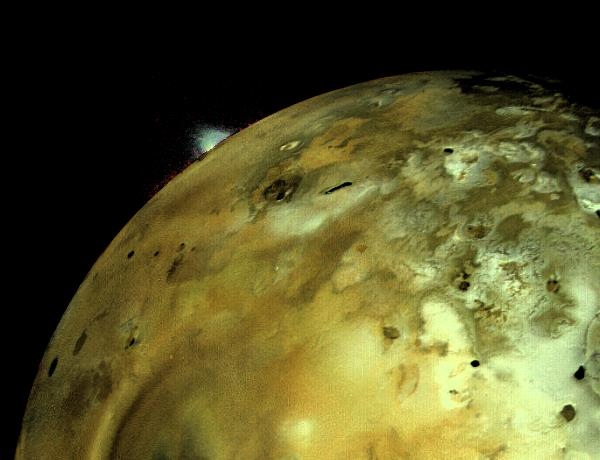
\includegraphics[width=0.8\linewidth]{revistas/002/imaxes/io.jpg}
    \captionof{figure}{Explosión do volcán Loki en Io.}
\end{center}

O 9 de novembro de 1980 sucede o encontro coa lúa máis grande de Saturno,
Titán, e co propio Saturno. Descúbrense Atlas, Prometeo e Pandora, tres
``pequenas'' lúas das máis de duascentas que actualmente se coñecen orbitando
este xigante gaseoso. As órbitas de Prometeo e Pandora ao redor dos aneis F de
Saturno confirman a teoría da existenca de ``satélites pastores'' que producen
ocos nos aneis e fixan gravitacionalmente os seus bordos. Recóllense vistas da
brillante superficie de Encélado e obsérvanse formas enigmáticas nos aneis de
Saturno que se pasarían a denominar radios, cuxa orixe non se comprende
completamente na actualidade.

\begin{center}
    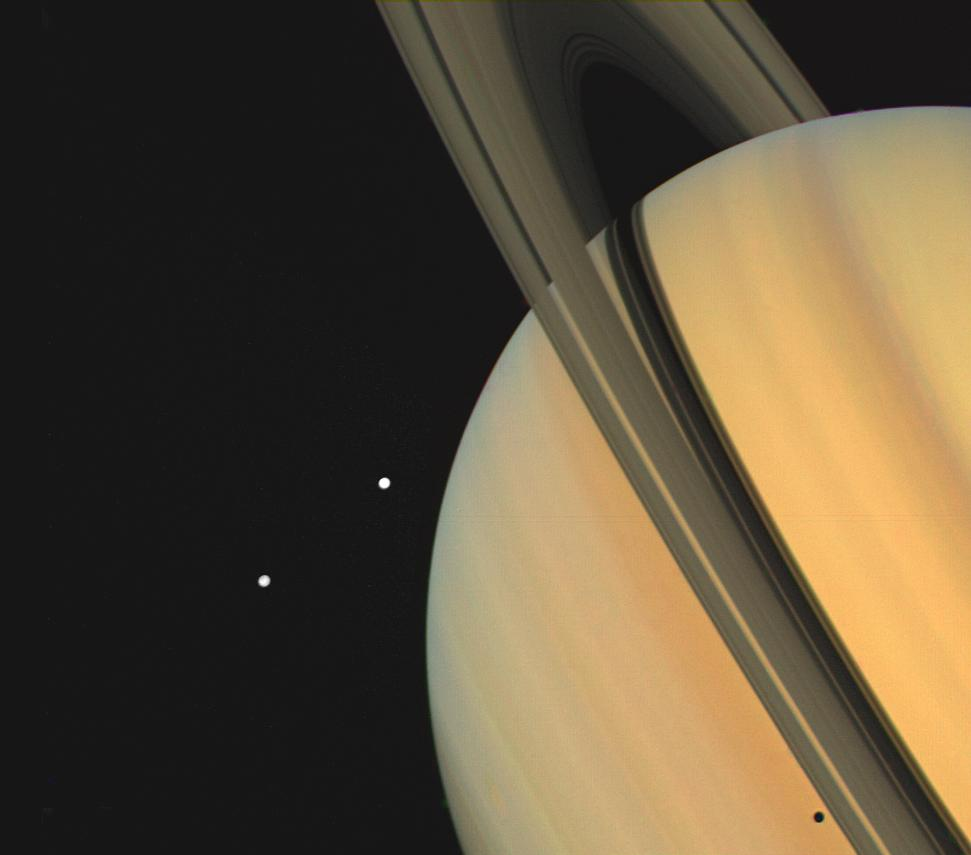
\includegraphics[width=0.8\linewidth]{revistas/002/imaxes/saturno.jpg}
    \captionof{figure}{Saturno con Tetis (arriba-dereita) e Dione. As
    sombras dos aneis e de Tetis proxéctanse nas nubes do planeta.}
\end{center}

\textbf{\textit{Life on Titan?}}

Titán é a segunda lúa máis grande do sistema solar tras Ganímedes e tamén é o
único lugar do sistema solar á parte do noso planeta en cuxa superficie se pode
atopar líquido estable en forma de ríos, lagos e mares. A súa densa atmosfera
neboenta e dourada está composta principalmente por nitróxeno e pequenas
cantidades de metano e etano. Os sinais de radio recibidos da Voyager 1
permitiron descubrir a existencia dunha superficie xeada en Titán, baixo a cal
existe un océano formado principalmente por auga que podería albergar formas de
vida, quizais a escala microscópica. Tan igual de plausible é que non haxa vida
en Titán. A misión \textit{Dragonfly} enviará unha aeronave rotatoria robótica,
será lanzada en xullo de 2028 e chegará a Titán en 2034.
\begin{center}
    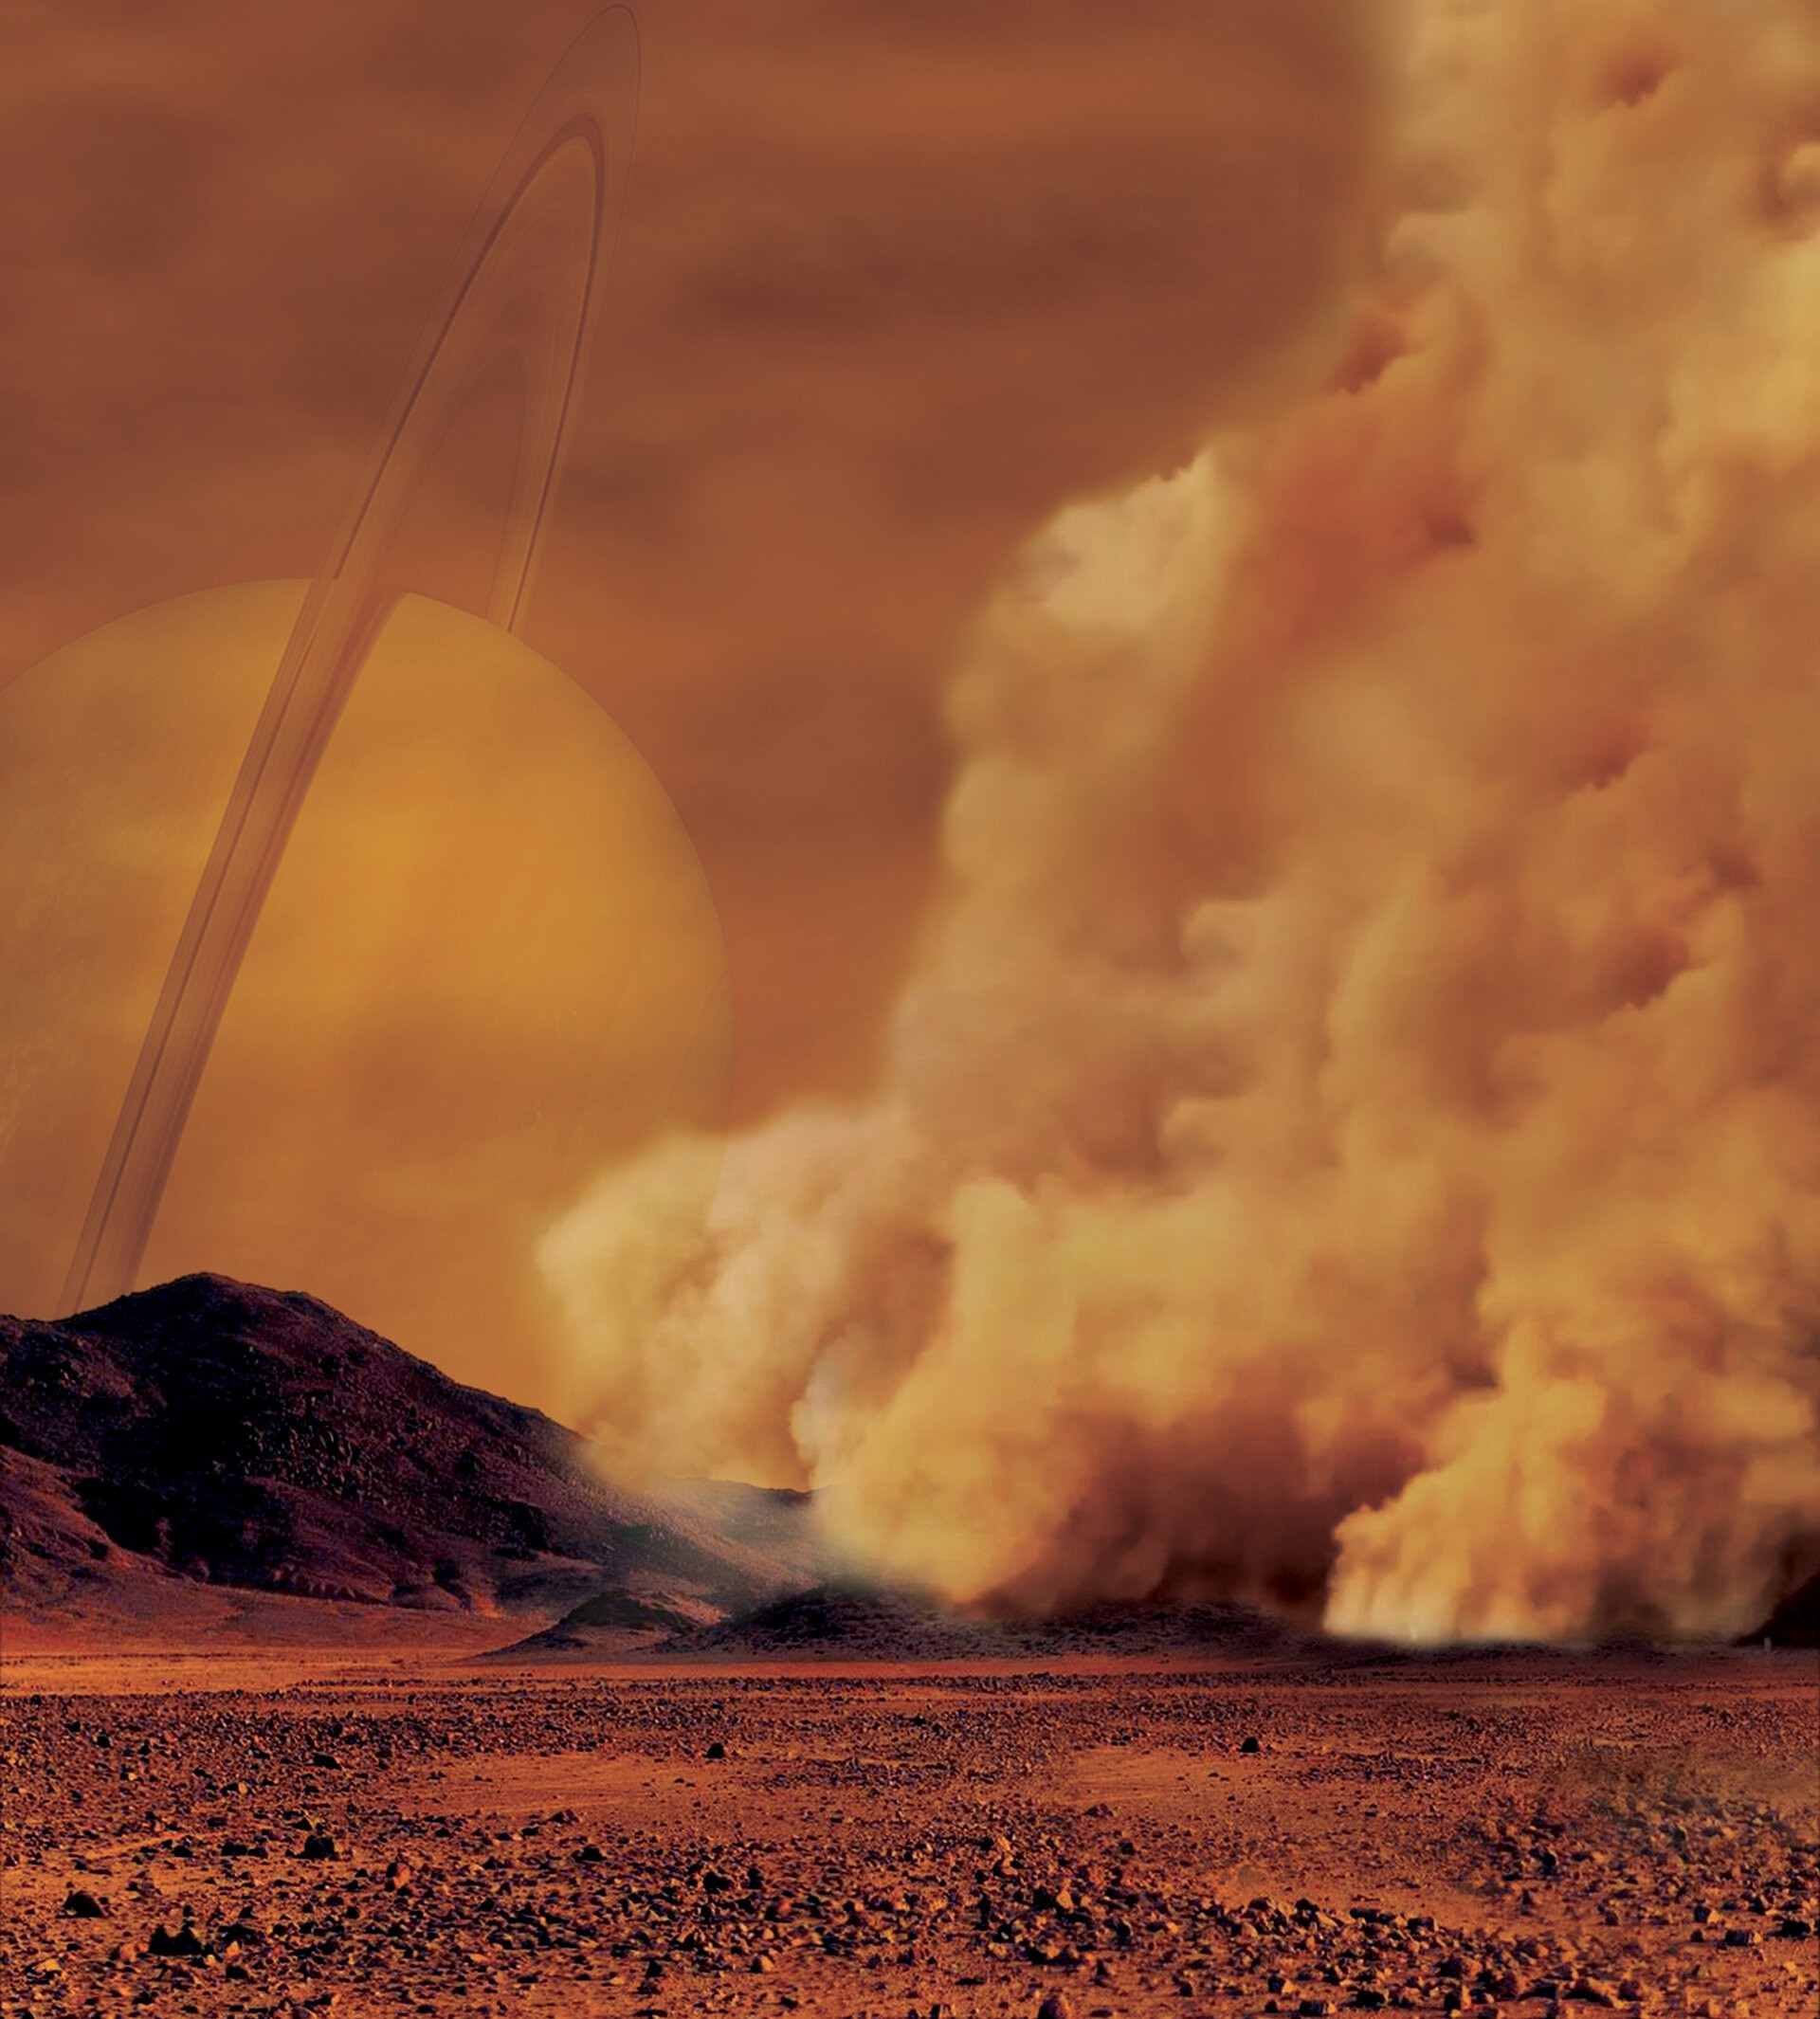
\includegraphics[width=0.6\linewidth]{revistas/002/imaxes/Dust_storm_on_Titan_pillars_corte.jpg}
    \captionof{figure}{Concepción artística de unha tormenta de pó en Titán con Saturno de fondo.}
\end{center}


\subsection*{Misión estendida. Saíndo do sistema solar.}



O 14 de novembro de 1980 comeza a misión extendida da Voyager 1. Recibindo un
impulso gravitacional, a sonda comeza a alonxarse do plano da eclíptica do
sistema solar e dez anos máis tarde, o 14 de febreiro de 1990, toma o
\textit{Retrato de familia} do sistema solar a petición do astrónomo Carl
Sagan: un mosaico composto de sesenta cadros individuais, as últimas imaxes
capturadas pola Voyager 1 antes de apagar a súa cámara ISS para sempre. A
Voyager 1 xa non voará preto de ningún outro obxecto astronómico en todo o
tempo no que durará o seu subministro enerxético polo que se prioriza o uso
deste en tarefas de recolección de datos do vento solar e do espazo
interestelar. A estas alturas, os febles sinais das sondas Voyager son
capturadas pola \textit{Deep Space Network} da NASA, con complexos en Goldstone
(California), Madrid e Canberra (Australia) que albergan grandes antenas de ata
setenta metros de diámetro.

\begin{center}
    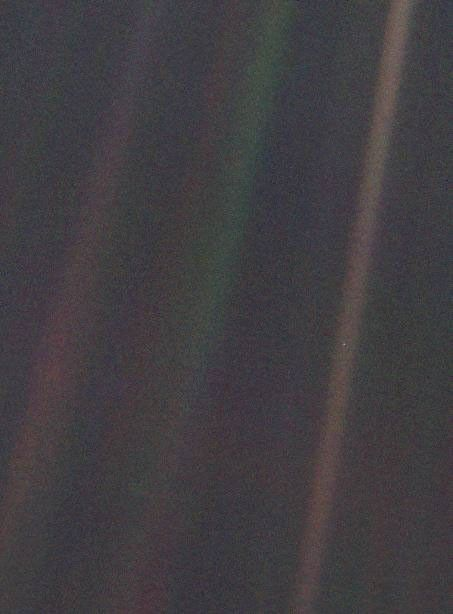
\includegraphics[width=0.6\linewidth]{revistas/002/imaxes/PaleBlueDot.jpg}
    \captionof{figure}{\textit{Pale Blue Dot}: imaxe da Terra tomada
        pola Voyager 1 para o \textit{Retrato de familia}. A Terra, vista
        a unha distancia de seis mil millóns de quilómetros, aparece coma
    un pequeno punto azulado na franxa vermella da dereita. }
\end{center}

O 17 de febreiro de 1998 a Voyager 1 sobrepasa a distancia do Pioneer 10 e
convírtese no obxecto feito polos humanos máis afastado da Terra, a unha
distancia de dez mil millóns de quilómetros. En decembro de 2004 a Voyager
alcanza a fronte de choque de terminación. Este é o límite coa última gran
rexión de dominio do vento solar, a heliosfera. O 25 de agosto de 2012 a
Voyager 1 convértese no primeiro obxecto humano no espazo interestelar
atravesando a fronteira da heliosfera, coñecida co nome de heliopausa. A
Voyager 1 ``escoitou'' os \textit{sons interestelares}. Vibracións do denso
plasma interestelar permitiron medir por primeira vez a densidade do medio
interestelar. Grazas á nosa tecnoloxía podemos transformar esas vibracións
eléctricas do plasma en zumbidos agudos e inquedantes que provocan calafríos.

Entre 2021 e 2024 a Voyager enfrentou varios desafíos relacionados coa
corrupción de datos e a súa transmisión á Terra, probablemente pola degradación
da aparataxe
% como dicía na nota, esta palabra non existe e en tal caso sería masculina
tras décadas de exposición á radiación espacial. Deste ano nunha década se
espera que a Voyager xa non dispoña de enerxía para alimentar ningún dos
instrumentos a bordo e perderemos o seu sinal para sempre.\\

\textbf{\textit{Message in a bottle.}}\\
Agárdase que a Voyager 1 entre na nube de Oort nuns trescentos anos. Esta é a
rexión de procedencia dos cometas de período longo e está situada a case un ano
luz do Sol e a un cuarto da distancia deste a \textit{Próxima Centauri}, a
estrela máis cercana ao sistema solar. A sonda tardará uns trinta mil anos en
saír dela sen rumbo particular cara a ningunha estrela. Estará destinada a
errar por toda a eternidade a través da Vía Láctea. Pasará moito tempo
viaxando, lonxe de ningunha illa estelar e portando o \textit{Golden Record}.
As Voyager son un primeiro grito cheo de esperanza que a humanidade lanzou
dende a beira do océano cósmico para darse a coñecer, unha mensaxe que di
\textit{hai alguén aí?}. \\

<<\textit{Quizais os rexistros nunca sexan interceptados. Quizais ninguén en
cinco mil millóns de anos os atope. Cinco mil millóns de anos é moito tempo. En
cinco mil millóns de anos, todos os seres humanos extinguiranse ou
evolucionarán noutros seres, ningún dos nosos artefactos sobrevivirá na Terra,
os continentes alteraranse ou destruiranse de forma irrecoñecible e a evolución
do Sol queimará a Terra ata convertela en} `crumble' \textit{ou a reducirá a un
remuíño de átomos.\\ Lonxe do fogar, intactas por estes acontecementos remotos,
as Voyagers, portadoras das lembranzas dun mundo que xa non existe, seguirán
voando.}>>

\hfill Carl Sagan, \textit{Pale Blue Dot} (adaptación).  

 % ao igual que antes hai que cambiar a cita


\nocite{oliver-berry.dmagmmvs_2019}
\nocite{sagan.c_2014}
\nocite{science_nasa_mission_voyager_timeline}
\nocite{photojournal_jpl_voyager_1}
\nocite{nasa_nssdc_gsfc}


\printbibliography

\end{multicols}
\end{refsection}
\newpage
\Titular%
{Robert Hooke. Nunca vaias contra Newton}%
{Pablo Duarte López}%
{historia}%
{Sobre como se pode pasar de ser a gran figura da túa época a ser case esquecido.}

\begin{refsection}
\begin{multicols}{2}


A todos nesta facultade sóannos os grandes científicos da historia, levamos
escoitando falar dalgúns deles dende o instituto, ou incluso antes, Newton,
Hooke, Boyle e tantos máis levan anos roldando nas nosas mentes, mais coñecemos
realmente algo deles aparte dun par de fórmulas co seu apelido? Se quizais
nunca vos parastes a pensar na vida que hai detrás destas figuras, pódovos
asegurar que agochan historias moito máis interesantes do que un imaxinaría.
Neste pequeno artigo mostrareivos a vida de Robert Hooke porque, crédeme, fixo
moito máis ca estudar resortes.

\subsection*{Quen foi Robert Hooke?}

Seguro que este científico inglés non é ningún descoñecido para vós, despois de
todo, se estades nesta facultade nalgún momento tivestes que ver a famosa lei
da elasticidade que leva o seu nome: $F= -k\cdot\Delta x$. Malia que sexa a
principal razón pola que é coñecido pola maioría de nós a día de hoxe, a súa
contribución á ciencia do século XVII non foi cousa menor. Dende o seu traballo
como principal axudante nos laboratorios de Boyle ata a súa inestimable axuda á
hora de reconstruír a cidade tralo gran incendio de Londres de 1666, pandora

tamén pola astronomía e a cronometría; Hooke deixou a súa pegada nas distintas
áreas da ciencia e da enxeñaría do momento e ata chegou a ser nomeado
presidente da Royal Society.

\begin{figure}
    \centering
    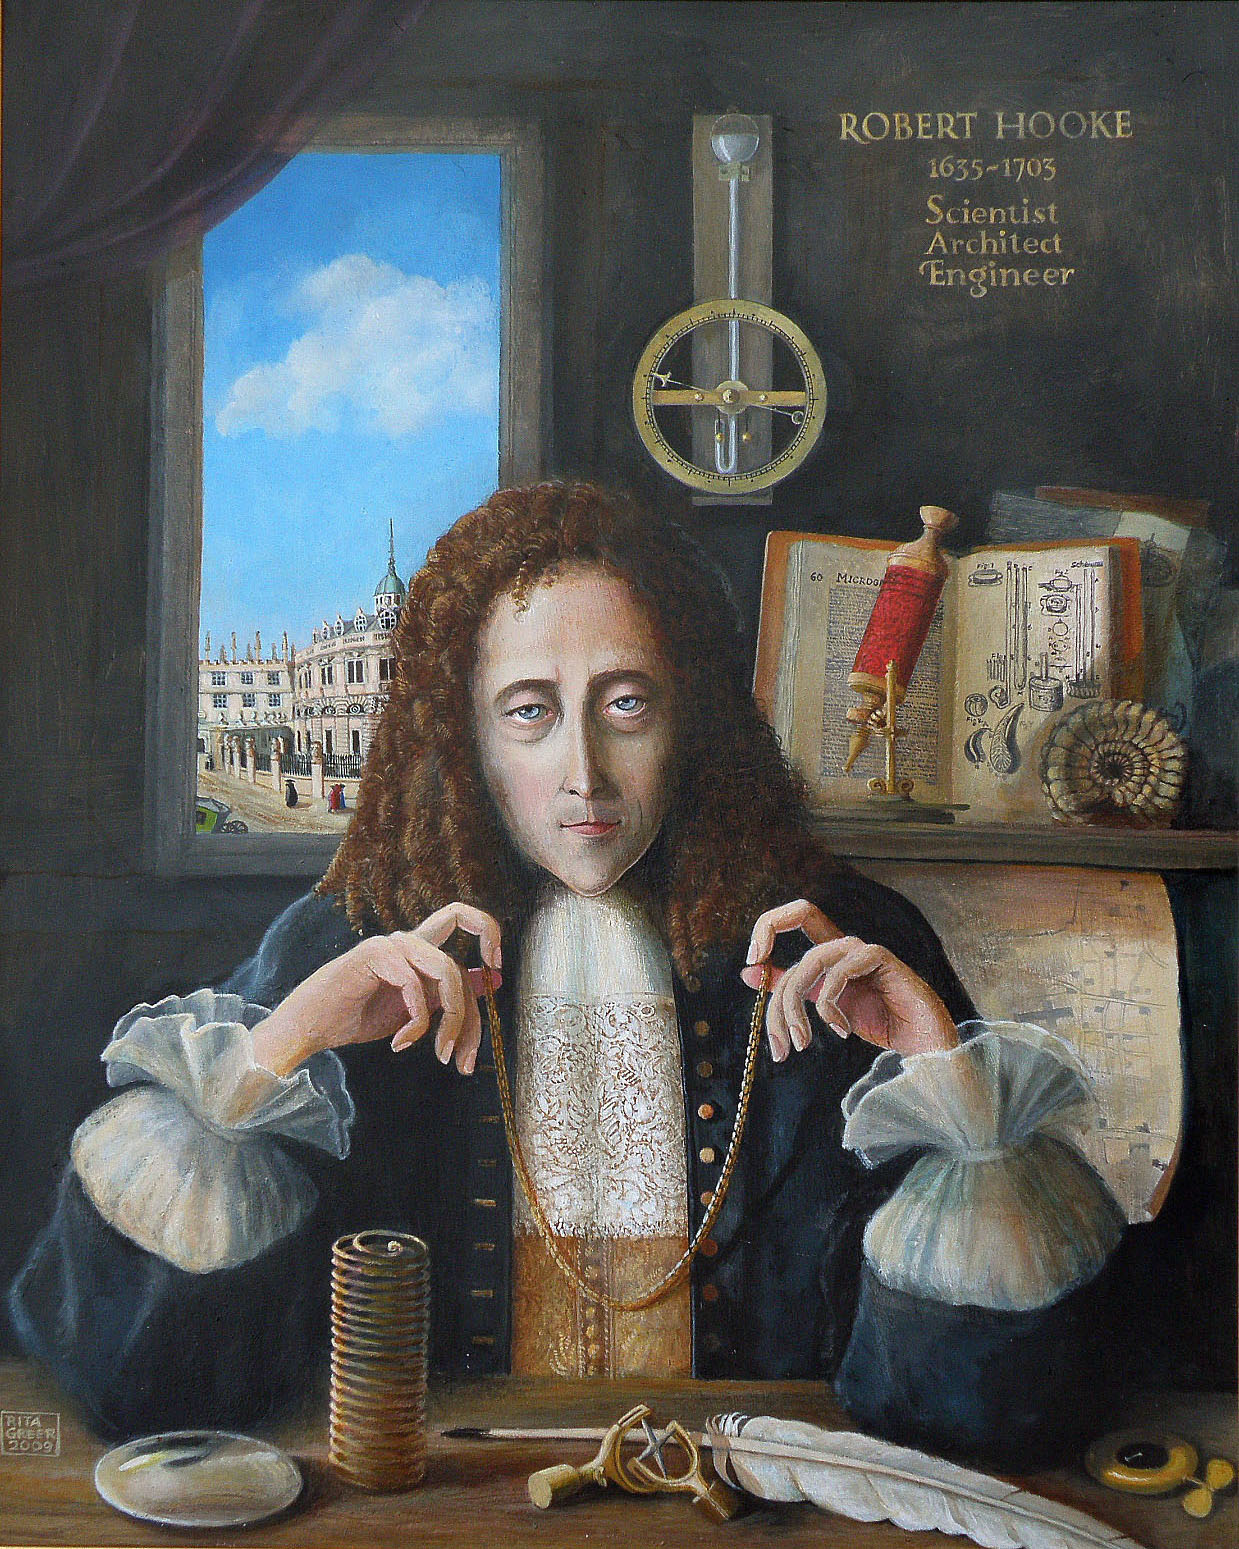
\includegraphics[width=0.8\linewidth]{revistas/002/imaxes/17_Robert_Hooke_Engineer.jpg}
    \captionof{figure}{Retrato póstumo de Robert Hooke. Rita Greer, FAL, via Wikimedia Commons}
\end{figure}

A súa \textit{magnum opus}, \textit{Micrographia}, supón un antes e un despois
no que a microscopía se refire, nela detállanse cincuenta e sete observacións
realizadas cun microscopio que o mesmo Hooke construíu, acompañadas por
detallados debuxos. Quizais, a achega máis destacada (e a razón pola que o
coñecerán os compañeiros e compañeiras da facultade de bioloxía) sexa que en
\textit{Micrographia} é onde se emprega por primeira vez o término ``célula''
ao describir unhas estruturas presentes nun anaco de cortizo. Esta obra, ao
estar escrita en inglés, na lingua vernácula (algo totalmente inusual para a
época), e non en latín, foi un escrito que recebiría a atención dos seus
coetáneos facilitando a accesibilidade; converteuse no primeiro \textit{best
seller} científico de todos os tempos.

\subsection*{Rivalidade con Newton}

Sereivos franco, se comecei a facer un artigo sobre a vida de Hooke non foi
polas súas múltiples achegas á ciencia, por moi interesantes e variadas que
estas fosen, senón pola continuada rivalidade que el tivo con nin máis nin
menos que Isaac Newton.

Todo comezou cando, pouco despois da publicación de \textit{Micrographia},
Newton comezou os seus propios experimentos coa luz, en concreto, o que fixo
botar chispas foi o estudo por parte de Newton do mesmo fenómeno que estudara e
describira Hooke por primeira vez na súa obra mestra. Este fenómeno trátase
dunha serie de aneis concéntricos que xorden ao pór en contacto dúas
superficies translúcidas, unha plana e outra curva.\footnote{Curiosamente, este
fenómeno coñécese como aneis de Newton, malia que non foi o primeiro en
describilos.} Isto non houbera suposto ningún problema de non ser porque Newton
en ningún momento lle deu a Hooke o crédito que este merecía por ser el o
descubridor do fenómeno. Foi así como iniciou a súa rivalidade, por unha banda,
Hooke, esixindo o crédito que merecía; pola outra, Newton, demasiado orgulloso
como para recoñecer que o seu traballo non foi totalmente orixinal. A situación
escalou durante anos, ata que a Royal Society, organización á que ambos
pertencían e da cal Hooke era presidente, veuse obrigada a intervir para evitar
que caese a reputación da mesma, polo que fixo que ambos tiveran unha
reconciliación pública. Foi neste contexto onde Newton, nunha carta a modo de
desculpa, escribe a súa tan aclamada frase <<Se puiden ver máis aló, foi porque
me encontraba sentado sobre os ombreiros duns xigantes>>.

Ben, paremos por un momento, porque isto foi o que me fixo escribir este artigo
nun primeiro lugar. Para dar contexto, Robert Hooke era un home pequeno,
corcovado e cunha deformación no lombo á raíz de diversos problemas na súa
infancia. Pois ben, disque, cando Newton escribiu a frase antes mencionada,
quixo tirar un último ataque público a Hooke, recoñece que toma o coñecemento
que achegaron os grandes sabios do pasado, eses ``xigantes'' dos que fala, pero
nunca de alguén coma Robert Hooke, quen, fisicamente, era de todo menos
xigante. Un pensaría que esta historia remataría aquí, cunha desculpa pública
de ambos e Newton tendo a última palabra, pero non, non será así.

\subsection*{Trala súa morte}

No momento en que morre Hooke, suceden dúas cousas: por unha banda, Newton
convértese en presidente da Royal Society; pola outra, publícase
\textit{Opticks}, unha extensa obra escrita por Newton sobre óptica, a cal
levaba varios anos sen publicar, agardando a morte de Hooke, para evitar
calquera posible crítica por parte deste\footnote{Newton defendía un modelo
corpuscular da luz mentres Hooke defendía o modelo ondulatorio, o que levou a
máis debates entre eles.}. Por se non for pouco, durante o cambio da sede da
Royal Society, supervisado por Newton, trasladáronse os cadros dos múltiples
presidentes que esta tivera; curiosamente, o único que nunca volveu a aparecer
foi o de Robert Hooke. Este era o único retrato que existía del, polo que non
se conserva ningunha imaxe del en vida.

Trala morte de Hooke, a súa figura como gran científico foi desaparecendo pouco
a pouco e as súas achegas fóronse minimizando ou atribuíndo a outros durante os
séculos posteriores. Non foi ata tempos relativamente recentes cando algúns
científicos e historiadores comezaron a reivindicar de novo a importancia da
súa figura na ciencia e na enxeñería, chegando a darlle o título de ``O
Leonardo da Vinci inglés''.

\begin{center}
    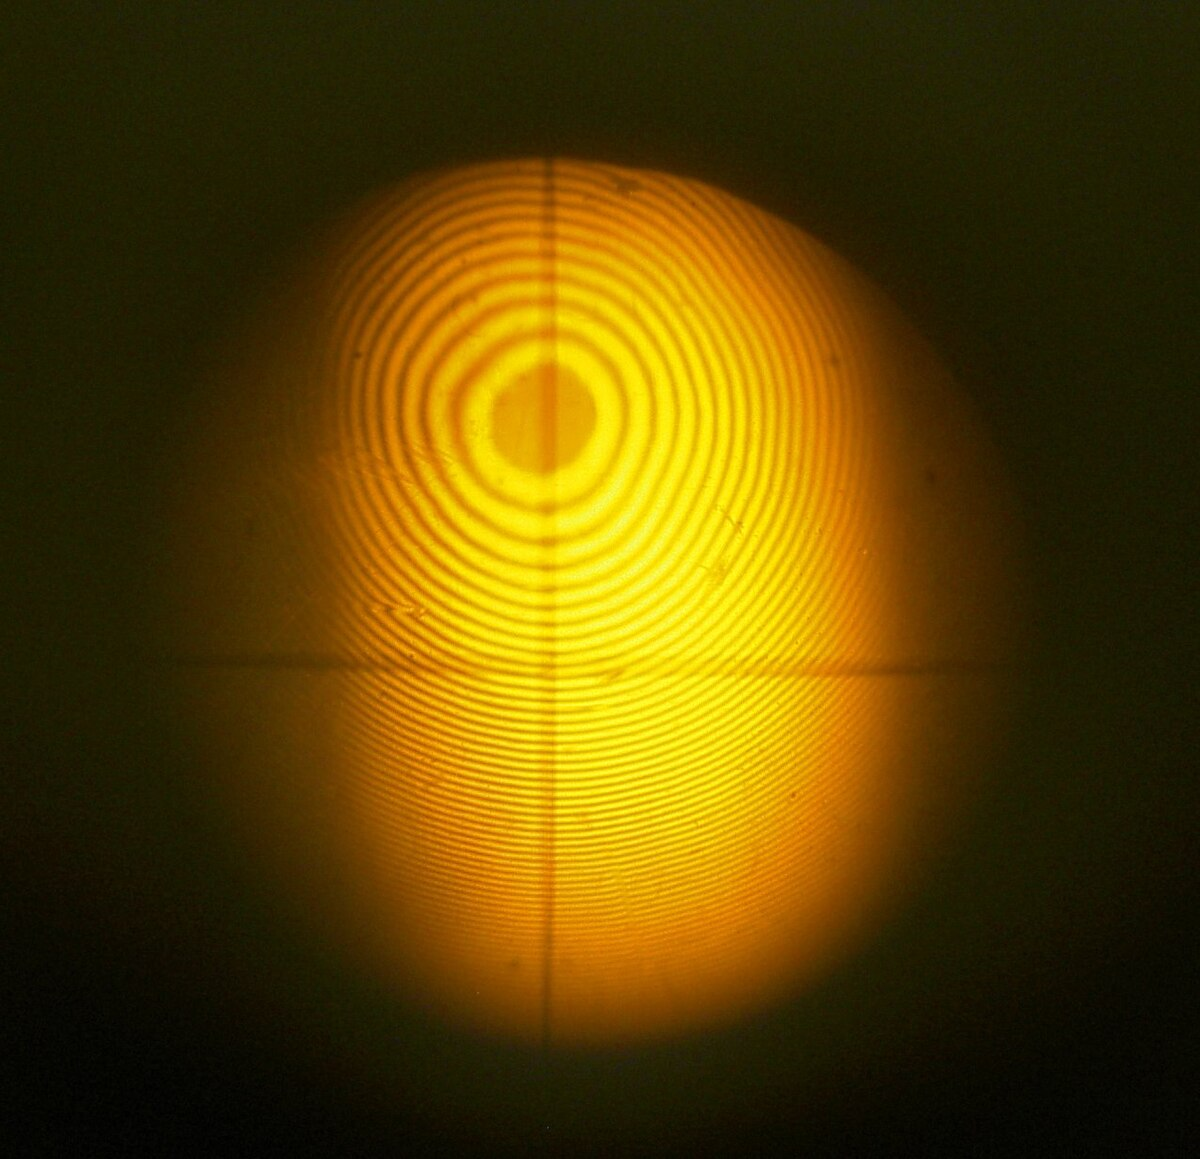
\includegraphics[scale=0.2]{revistas/002/imaxes/Newton-rings}
    \captionof{figure}{Exemplo dos \textit{aneis de Newton}. Imaxe de Wikipedia}
\end{center}

\nocite{gribbin2004historia}
\printbibliography

\end{multicols}
\end{refsection}
\newpage
\Titular%
{\textit{Strike, you're out!} Bombas, Heisenberg e un catcher}%
{Santiago González Gómez}%
{historia}%
{As vidas dun beisbolista e dun dos pais da Física Cuántica, cruzadas por unha
historia de espías e o proxecto atómico da Alemaña nazi.}%

\begin{refsection}
\begin{multicols}{2}

\subsection*{Heisenberg e o \textit{proxecto Uranio}}

Cando en setembro de 1939 estourara a Segunda Guerra Mundial, Werner
Heisenberg, un dos pais da física cuántica, foi requirido polo goberno nazi
xunto con outros destacados físicos alemáns. O estudo da fisión nuclear
atopábase en auxe e Alemaña quería estudar a viabilidade de construír unha
bomba que empregase este novo campo como elemento destrutivo. Comezaba así o
\textit{proxecto Uranio}, o análogo alemán ao \textit{proxecto Manhattan}
estadounidense.

A posición de Heisenberg era delicada. Aínda que se opoñía ao réxime nazi,
tamén era un fervente patriota alemán, e temía que unha derrota de Alemaña na
guerra resultase nunha ocupación soviética de Europa, algo que consideraba
bastante peor que o dominio nazi. Por outra banda, tampouco tiña moita elección
sobre a súa participación no proxecto; non só pola posibilidade de perder o seu
traballo, senón porque a súa relación con científicos xudeus antes da guerra
facíao sospeitoso a ollos de moitos nazis.

\begin{centering}
    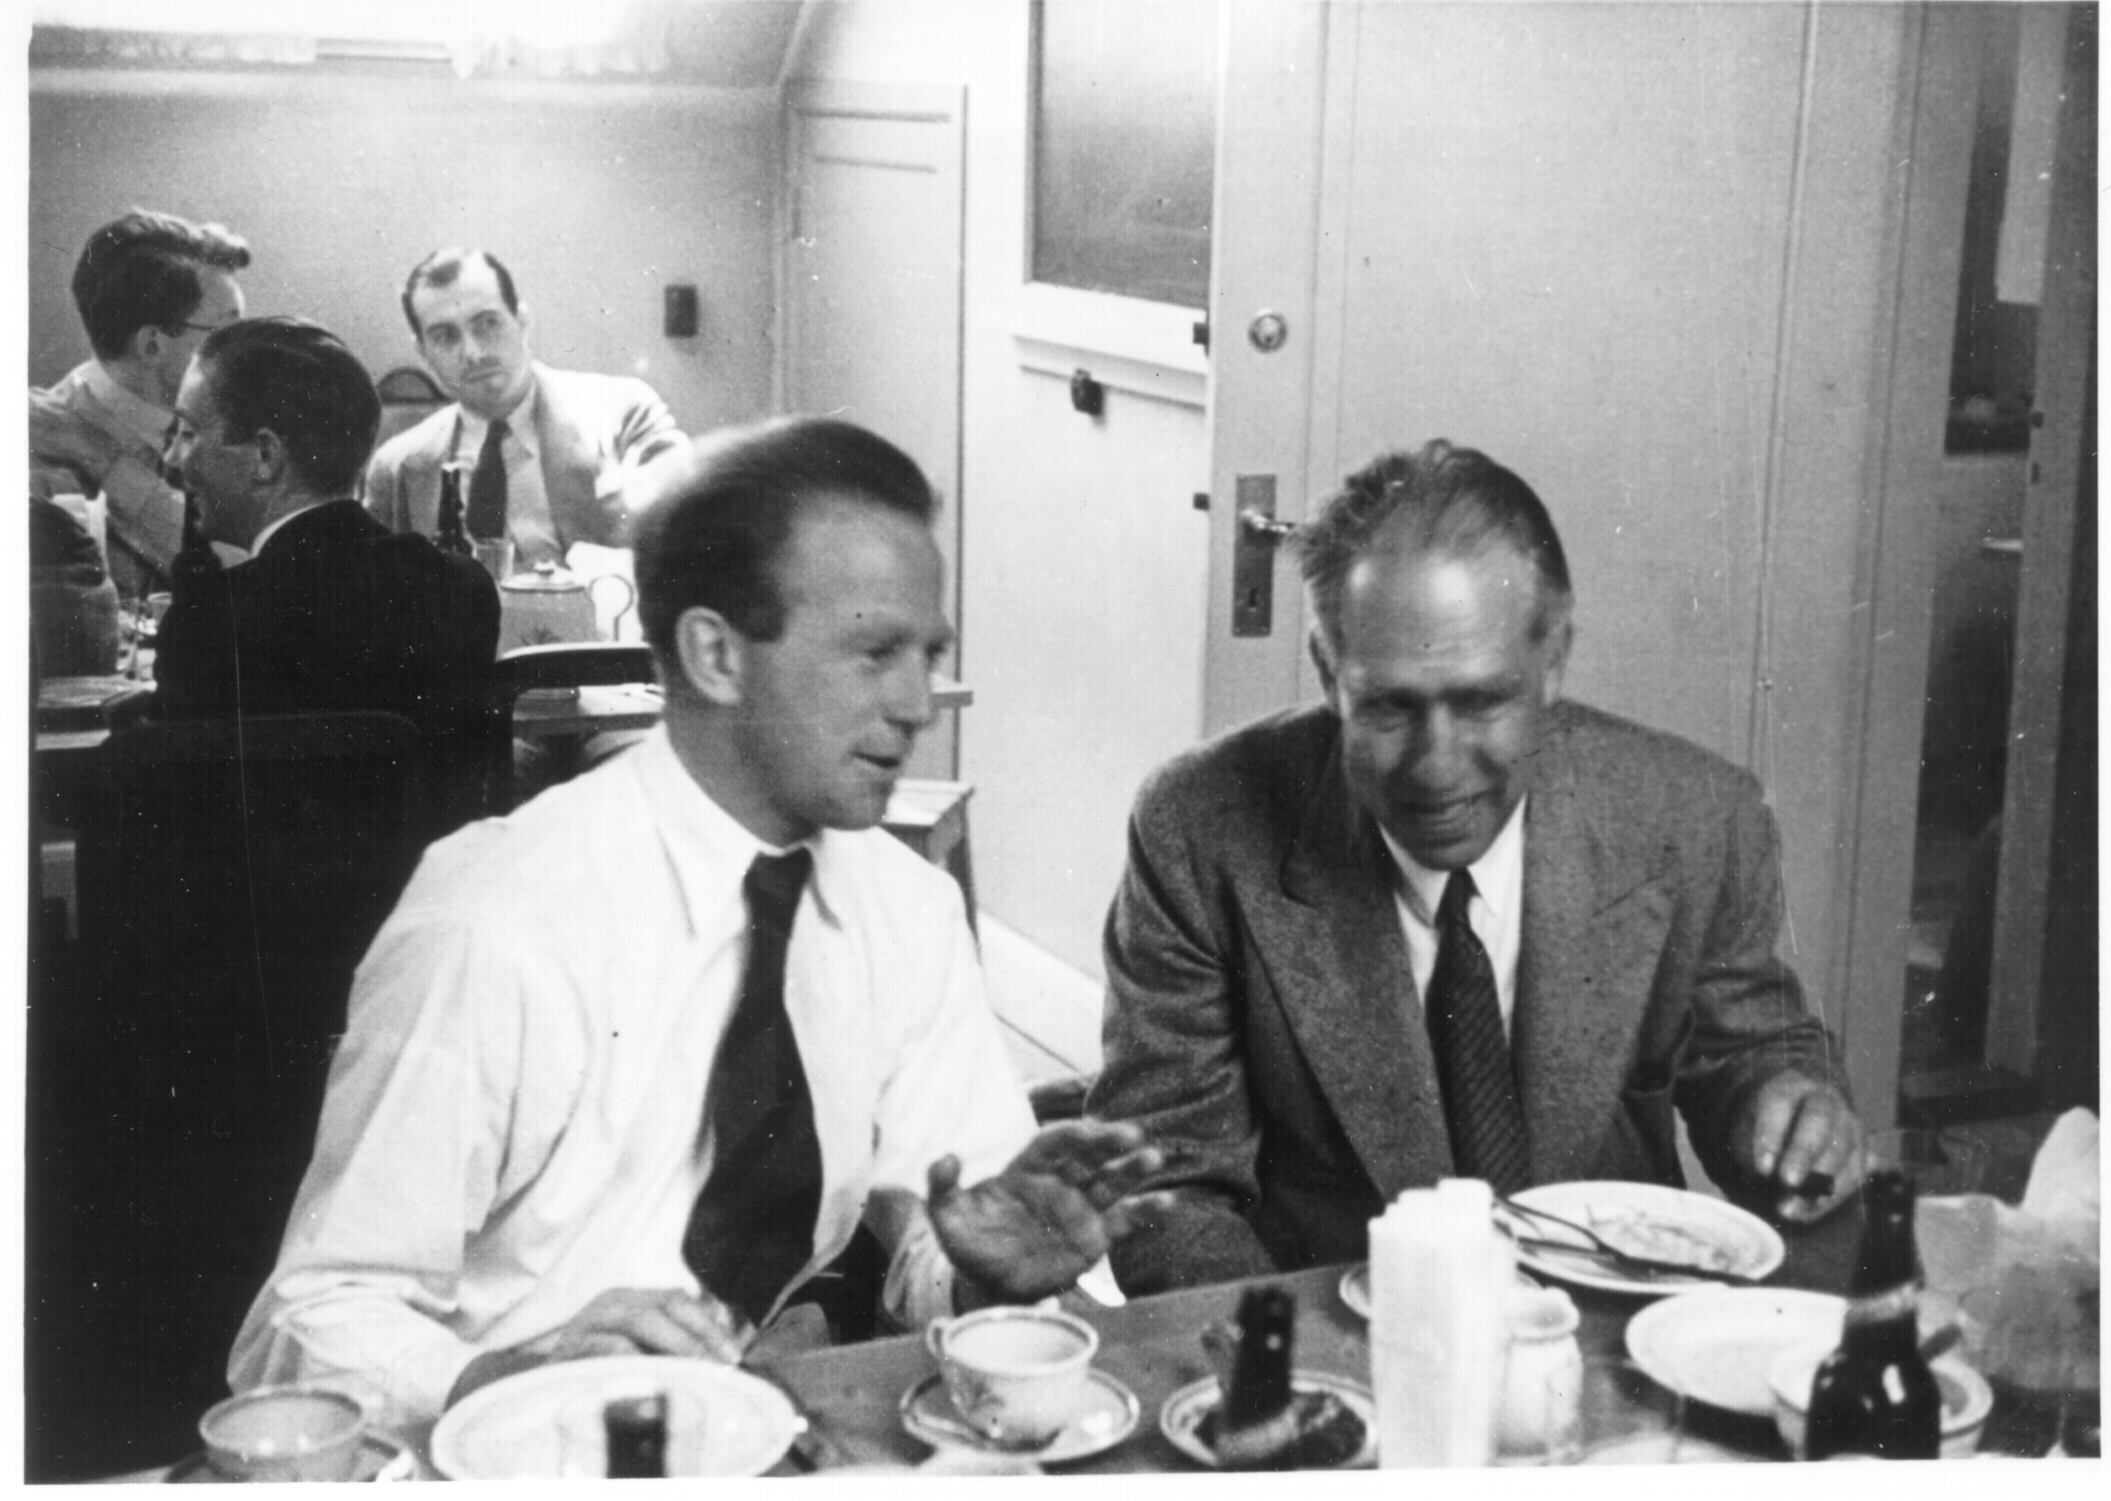
\includegraphics[width=0.65\linewidth]{revistas/002/imaxes/bohr.jpg}
    \captionof{figure}{Heisenberg e Bohr nun encontro en 1941. Imaxe do Niels Bohr Archive.}
\end{centering}

Sexa como for, Heisenberg pasara dous anos investigando intensamente ata
concluír, en 1941, que malia ser posible construír a bomba (tanto de uranio
como de plutonio), esta levaría demasiado tempo e consumiría demasiados
recursos alemáns. Heisenberg consideraba ademais que os rivais de Alemaña
chegarían ás mesmas conclusións. Os líderes nazis aceptaron a súa opinión e o
\textit{proxecto Uranio} pasou a investigar a posibilidade de construír un
reactor nuclear que producise enerxía eléctrica.

Para Heisenberg, o posible desenvolvemento dunha bomba nuclear supuña un dilema
moral importante, así que chegar a esta conclusión foi, dende logo, un alivio.
Porén, a idea (ou mellor dito, o medo) de ter que construír unha bomba nuclear
nun futuro nunca abandonou a súa cabeza. Aproveitando unha visita a Dinamarca,
deixou caer ao seu vello mentor Niels Bohr as súas dúbidas morais sobre a
producción de armamento atómico. Bohr creu que Heisenberg lle estaba a tender
algún tipo de trampa deseñada pola Gestapo e preferiu cambiar de tema.

\subsection*{``O home máis intelixente do béisbol''}

Para o ano 1942 e, ao outro lado do Atlántico, os Estados Unidos iniciaban o
seu propio programa atómico: o \textit{proxecto Manhattan}. Pero remontémonos
algo máis atrás no tempo...

En 1934, un equipo de \textit{all-stars} do béisbol estadounidense fixo unha
xira por Xapón, onde o béisbol comezaba a ser un deporte cada vez máis popular.
Xunto a todas as estrelas, viaxou co equipo un \textit{catcher} mediocre, que
levaba anos saltando de equipo a equipo na liga sen destacar especialmente: Moe
Berg. Berg, de orixe xudía, ten sido descrito como ``o beisbolista máis estraño
da historia'' ou ``o home máis intelixente do béisbol''. Aínda que non era un
xogador especialmente destacado, si era tremendamente astuto, e tiña unha
habilidade innata para os idiomas, de aí que estudara a fondo polo menos sete
diferentes. Precisamente, a razón pola que Berg viaxara a Xapón en 1934 era
pola súa capacidade para falar xaponés.

Cando os Estados Unidos entraran na Segunda Guerra Mundial, Berg alistouse e
pasou por varios destinos lonxe da fronte. En 1943, uniuse á OSS, a precursora
da actual CIA, onde fora moi valorada a súa capacidade para os idiomas. Berg
realizou primeiramente varias misións como espía en Iugoslavia, onde
investigaba grupos partisanos que os Estados Unidos consideraba apoiar.

Cara a 1943, Berg comezou a traballar no \textit{proxecto Larson}, unha
operación cuxo obxectivo inicial era reclutar a físicos italianos e levalos aos
Estados Unidos para que colaborasen no \textit{proxecto Manhattan} e outras
misións armamentísticas. Berg acabou por percorrer varios lugares de Europa
entrevistando a físicos, non só para tentar convencelos de que se mudasen aos
Estados Unidos, senón tamén para obter información sobre Heisenberg. Os
estadounidenses sospeitaban que Heisenberg dirixía un proxecto atómico para os
alemáns, e despois de que Bohr, a quen os aliados sacaron de Dinamarca en 1943
e levaron a Reino Unido para que colaborase con eles, comentase as
conversacións que Heisenberg tivera con el en 1941; era indispensable
determinar como de preto estaba o alemán de desenvolver a temida bomba. A OSS
chegou a considerar a posibilidade de secuestralo, pero isto nunca chegou a
suceder.

\begin{centering}
    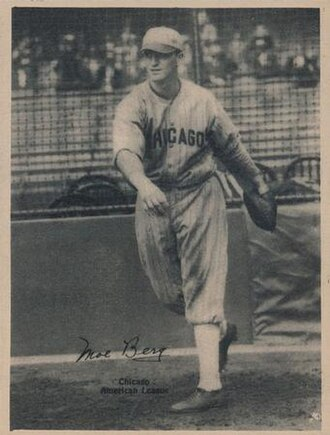
\includegraphics[width=0.55\linewidth]{revistas/002/imaxes/bergChicago.jpg}
    \captionof{figure}{Cromo de Berg mentres xogaba para os Chicago White Sox. Imaxe de Wikipedia.}
\end{centering}

En 1944, a OSS soubo que Heisenberg ía dar unha conferencia en Zürich,
territorio neutral. A Berg, que por suposto falaba alemán, asignóuselle a
misión de asistir á dita conferencia e tentar determinar se este estaba preto
de construír a bomba atómica. Se o espía contara coa máis mínima sospeita de
que Heisenberg supoñía un perigo, tiña ordes de levantarse no medio da
conferencia e dispararlle.

Berg non só acudira á conferencia facéndose pasar por estudante de física,
senón que tamén estivo presente nunha festa á que o teórico alemán asistira na
súa estancia en Zürich. O beisbolista saíu do evento á vez que Heisenberg e
entablou diálogo con el no camiño de volta; non houbo nada nestas conversas que
fixese sospeitar a Berg. O patriota alemán admitira durante a festa que a
guerra estaba perdida para os alemáns, algo que Berg xulgou que non diría
alguén que estaba a piques de rematar unha bomba atómica. Tamén reflexionou
que, aínda que tería sentido matar a Heisenberg en 1942 nos inicios dun suposto
proxeto de bomba atómica alemá, para o 1944 xa sería demasiado tarde.
Finalmente, decidiu non asasinar a Heisenberg e as súas vidas separáronse para
non volver a atoparse nunca máis.

\subsection*{Unha granxa en Cambridge}

Moito se ten discutido sobre o papel de Heisenberg no \textit{proxecto Uranio},
considerando que o \textit{proxecto Manhattan} si foi exitoso. De verdade
tentou fabricar a bomba e simplemente non o conseguiu por incompetencia? Ou
saboteou o \textit{proxecto Uranio} por motivos morais, convencendo ao resto
dos seus integrantes da imposibilidade de construír a bomba?

Esta dúbida tamén asaltou aos estadounidenses cando en 1945 capturaron a
Heisenberg e o resto de físicos alemáns do \textit{proxecto Uranio}. Todos eles
foron trasladados á \textit{Farm Hall}, unha mansión campestre inglesa preto de
Cambridge que estaba infesta de micrófonos para espiar as súas conversas. O 6
de agosto, os aliados aseguráronse de que Heisenberg e os demais escoitasen a
transmisión de radio do bombardeo de Hiroshima. Heisenberg inicialmente negouse
a crer que a bomba fose atómica, argumentando que a masa crítica (a masa mínima
de material radioactivo necesario para soster a reacción nuclear) necesaria
para unha bomba desas características debía ser dúas toneladas polo menos,
imposible de fabricar para os estadounidenses. Para decatarse do errado desta
afirmación, nótese que a bomba detonada posteriormente sobre Nagasaki contiña
64 kg de uranio enriquecido.

Que ocorreu? Mentía Heisenberg ao réxime nazi dando un valor falso da masa
crítica para impedir a fabricación da bomba? Non é tan sinxelo. Días despois,
fixo os cálculos e expuxo aos seus compañeiros como cría que os estadounidenses
fabricaran a bomba, estes cálculos resultaron ser moi correctos. Os físicos do
\textit{proxecto Manhattan} concluíron que o alemán simplemente \textit{nunca
antes realizara os cálculos} da masa crítica. Heisenberg estaba moito máis
interesado no desenvolvemento dun reactor que no dunha bomba e, imaxinándose un
valor desorbitado para a masa crítica, simplemente decidiu non facer os
cálculos. Posiblemente prefiría vivir no descoñecemento a afrontar o dilema
moral da construción da bomba.

Dende logo, ás veces é abrumador pensar como as decisións do individuo menos
esperado son capaces de cambiar o rumbo da historia.

\nocite{gottstein.k_2016}
\nocite{dawidoff.n_2011}

\printbibliography

\end{multicols}
\end{refsection}
\newpage
\Titular*%
{Pasatempos}%
{Luis Arcas, Víctor Díaz Díaz}%
{pasatempos}%
{}%
\vspace*{-6mm}
\section*{\textcolor{Resalte}{Encrucillado \#1}, Luis Arcas}

%{\CorResalte Encrucillado}
% Descomentar para entrar no modo solución
% No modo solución todos os puzzles saen resoltos
% \PuzzleSolution
\begin{Puzzle}{27}{16}
|[1]P  |{}    |{}    |{}    |{}    |{}    |{}    |{}    |{}    |{}    |{}    |{}    |{}    |{}    |{}    |{}    |{}    |[2]P  |{}    |{}    |{}    |{}    |{}    |{}    |{}    |{}    |{}   |{} |.
|É     |{}    |{}    |{}    |{}    |{}    |{}    |{}    |{}    |{}    |{}    |{}    |{}    |{}    |{}    |{}    |{}    |O     |{}    |{}    |[3]C  |{}    |{}    |{}    |{}    |[4]F  |{}   |{} |.
|N     |{}    |{}    |[5]L  |U     |[6]Z  |{}    |{}    |{}    |{}    |{}    |{}    |{}    |{}    |{}    |{}    |{}    |[7]I  |N     |T     |E     |N     |S     |I     |D     |A     |D    |E  |.
|D     |{}    |{}    |{}    |{}    |E     |{}    |{}    |{}    |{}    |[8]C  |{}    |{}    |{}    |{}    |{}    |{}    |S     |{}    |{}    |R     |{}    |{}    |{}    |{}    |S     |{}   |{} |.
|U     |{}    |{}    |[9]É  |T     |E     |R     |{}    |{}    |[10]G |R     |I     |F     |[11]F |I     |T     |H     |S     |{}    |{}    |N     |{}    |{}    |{}    |{}    |E     |{}   |{} |.
|L     |{}    |{}    |{}    |{}    |M     |{}    |{}    |{}    |{}    |I     |{}    |{}    |Í     |{}    |{}    |{}    |O     |{}    |{}    |{}    |{}    |{}    |{}    |{}    |S     |{}   |{} |.
|[12]O |S     |[13]C |I     |L     |A     |D     |O     |R     |E     |S     |{}    |{}    |S     |{}    |{}    |{}    |[14]N |E     |W     |T     |O     |N     |{}    |{}    |{}    |{}   |{} |.
|{}    |{}    |U     |{}    |{}    |N     |{}    |{}    |{}    |{}    |T     |{}    |{}    |I     |{}    |{}    |{}    |{}    |{}    |{}    |{}    |{}    |{}    |{}    |{}    |{}    |{}   |{} |.
|{}    |{}    |A     |{}    |{}    |{}    |{}    |{}    |{}    |{}    |A     |{}    |{}    |C     |{}    |{}    |{}    |{}    |{}    |{}    |{}    |{}    |{}    |{}    |{}    |{}    |{}   |{} |.
|[15]V |E     |N     |U     |S     |{}    |{}    |{}    |[16]V |O     |L     |F     |R     |A     |[17]M |I     |O     |{}    |{}    |[18]C |{}    |{}    |{}    |{}    |{}    |{}    |{}   |{} |.
|{}    |{}    |T     |{}    |{}    |{}    |{}    |{}    |{}    |{}    |{}    |{}    |{}    |{}    |O     |{}    |{}    |{}    |{}    |A     |{}    |{}    |{}    |{}    |{}    |{}    |{}   |{} |.
|{}    |{}    |O     |{}    |{}    |{}    |{}    |{}    |{}    |{}    |{}    |{}    |{}    |[19]U |M     |A     |{}    |{}    |{}    |U     |{}    |{}    |{}    |{}    |{}    |{}    |{}   |{} |.
|{}    |{}    |{}    |{}    |{}    |{}    |{}    |{}    |{}    |{}    |{}    |{}    |{}    |{}    |E     |{}    |{}    |{}    |{}    |S     |{}    |{}    |{}    |{}    |{}    |{}    |{}   |{} |.
|{}    |{}    |{}    |{}    |{}    |{}    |{}    |{}    |{}    |{}    |{}    |{}    |{}    |[20]I |N     |E     |R     |C     |I     |A     |{}    |{}    |{}    |{}    |{}    |{}    |{}   |{} |.
|{}    |{}    |{}    |{}    |{}    |{}    |{}    |{}    |{}    |{}    |{}    |{}    |{}    |{}    |T     |{}    |{}    |{}    |{}    |{}    |{}    |{}    |{}    |{}    |{}    |{}    |{}   |{} |.
|{}    |{}    |{}    |{}    |{}    |{}    |{}    |{}    |{}    |{}    |{}    |{}    |{}    |{}    |O     |{}    |{}    |{}    |{}    |{}    |{}    |{}    |{}    |{}    |{}    |{}    |{}   |{} |.
\end{Puzzle}

\begin{PuzzleClues}{\textbf{Vertical}}
\Clue{1}{PÉNDULO}{O legado de Foucault na facultade}
\Clue{2}{POISSON}{Probablemente un peixe manchado}
\Clue{3}{CERN}{Centro de investigación europeo máis internacional}
\Clue{4}{FASES}{Son lunares ou diagramas}
\Clue{6}{ZEEMAN}{Ver dobre en cuántica débese a este efecto}
\Clue{8}{CRISTAL}{Disposición atómica ordenada}
\Clue{11}{FÍSICA}{Rama científica especializada no estudo da natureza e comportamento da materia, así como a forza e a enerxía}
\Clue{13}{CUANTO}{Canta enerxía?}
\Clue{17}{MOMENTO}{Teno esta revista}
\Clue{18}{CAUSA}{Precede ao efecto non relativista}
\end{PuzzleClues}

\begin{PuzzleClues}{\textbf{Horizontal}}
\Clue{5}{LUZ}{Onda e corpúsculo}
\Clue{7}{INTENSIDADE}{Voltaxe = ... $\times$ Resistencia}
\Clue{9}{ÉTER}{Se non se sabe o que é, posiblemente é isto}
\Clue{10}{GRIFFITHS}{O gran libro (polo menos en EM)}
\Clue{12}{OSCILADORES}{En esencia, todo son ... (pl.)}
\Clue{14}{NEWTON}{Físico nacido en Natividad}
\Clue{15}{VENUS}{Afrodisíaco planeta}
\Clue{16}{VOLFRAMIO}{Elemento W}
\Clue{19}{UMA}{Unidad de masa atómica}
\Clue{20}{INERCIA}{Principio de ..., o primeiro de tres}
\end{PuzzleClues}

%Causa • CERN • Cristal • Cuanto • Fases • Física • Griffiths • Inercia •
%Intensidade • Luz • Momento • Newton • Osciladores • Poisson • Péndulo • UMA •
%Venus • Volframio • Zeeman • Éter

% Solucions cifradas con rot13 (movendo os caracteres 13 adiante) 
% Pnhfn PREA Pevfgny Phnagb Snfrf Sífvpn Tevssvguf Varepvn Vagrafvqnqr Yhm
% Zbzragb Arjgba Bfpvynqberf Cbvffba Céaqhyb HZN Irahf Ibysenzvb Mrrzna Égre

\section*{\textcolor{Resalte}{Colgando cadros}, Víctor Díaz Díaz
}

% Título
%Colgando cadros
%
% Autor
%Víctor Díaz Díaz

% Corpo
\begin{refsection}
\begin{multicols}{2}

\subsection*{Enunciado}

Queremos colgar un cadro dunha parede empregando $n$ cravos, de xeito que
quitando \textbf{un único cravo calquera} o cadro caia polo seu peso, ignorando
fricción. Para o caso $n=1$, a solución sería a mostrada na figura \textbf{AQUI
HAI QUE POÑER A FIGURA CA SOLUCION}
% \ref{fig:sol_n1}.

\begin{itemize}
    \item[$\bullet$] Nivel básico: $n=2$.
    \item[$\bullet$] Nivel avanzado: $n=3$.
    \item[$\bullet$] Nivel experto: $n$ arbitrario.
\end{itemize}


\subsection*{Criterios de éxito}

\begin{itemize}
    \item[$\bullet$] Nivel básico: solución gráfica ou solución formal.
    \item[$\bullet$] Nivel avanzado: solución gráfica ou solución formal.
    \item[$\bullet$] Nivel experto: solución formal.
\end{itemize}

Nótese que hai varias solucións posibles para o Nivel experto.

\subsection*{Solucións}

\subsubsection*{Solucións gráficas}

\begin{itemize}
    \item[$\bullet$] Nivel básico: véxase a figura 1(b) de \cite{Demaine_2013}.
    \item[$\bullet$] Nivel avanzado: véxase a figura 4(c) de \cite{Demaine_2013}.
    \item[$\bullet$] Nivel experto: ningunha.
\end{itemize}

\subsubsection*{Solución formal}

A solución ao problema fai uso de conceptos de teoría de grupos, concretamente
de grupos libres. Todo o que se vai discutir a continuación foi extraído de
\cite{Demaine_2013}.

Dado un conxunto de $n$ elementos $C(n) = {x_i / i=1,2,...,n}$, denominados
\textit{xeradores}, contrúese un \textit{grupo libre} $F_C = (C(n),\cdot)$ a
partir de todas as palabras que se poden formar operando os xeradores $x_i$ e
os seus inversos $x_i^{-1}$. Deste xeito tamén definimos a identidade como $e =
x_i \cdot x_i^{-1}, \forall i$ (en adiante omitiremos o símbolo da operación).

No noso caso, $n$ será igual ao número de cravos e cada elemento de $C(n)$
corresponderáse coa forma de facer pasar a corda ao redor do cravo: $x_i$
representa un xiro ao redor do cravo $i$-ésimo no sentido horario, $x_i^{-1}$
representa un xiro ao redor do cravo $i$-ésimo no sentido antihorario e a
identidade $e$ correspóndese con non facer ningún xiro. Así, podemos escribir
cada xeito de colgar o cadro cunha palabra de $F_C$ e o noso obxectivo e atopar
aquelas palabras para as que, eliminando os $x_i$ e $x_i^{-1}$ para un $i$
concreto, a palabra resultante se simplifique ata corresponderse coa
identidade.

Para $n=1$, as únicas posibles palabras son $S_1 = x_1$ ou $S'_1=x_1^{-1}$,
aínda que realmente $S'_1 = (S_1)^{-1}$. Esto vai pasar para cada solución que
atopemos, e débese ao feito de que $S_n$ e $S_n^{-1}$ se corresponden ca mesma
forma de colgar o cadro, simplemente cambiando o sentido no que se recorren os
cravos. Neste caso é evidente comprobar que eliminar $x_1$ nos deixa sen
palabra, e o cadro cae.

Para $n=2$, a cantidade de palabras que se poden construir aumenta. Sen
embargo, non é complicado comprobar por forza bruta que a palabra $S_2 = x_1
x_2 x_1^{-1} x_2^{-1}$ é a solución ao problema. De novo, eliminando o cravo
$i$-ésimo suprimimos os $x_i$ e $x_i^{-1}$ da palabra, o que produce $x_1
x_1^{-1} = x_2 x_2^{-1} = e$, e o cadro cae. De cara a xeralizar o resultado
para $n>2$, cómpre notar que a palabra $S_2$ se corresponde co
\textit{conmutador} de $x_1$ e $x_2$ (ollo, a pesar de chamarse igual a súa
definición en teoría de grupos é diferente á empregada en física cuántica).
Teremos entón $S_2 = [x_1,x_2] = x_1 x_2 x_1^{-1} x_2^{-1}$.

Para $n>2$, a solución constrúese de xeito recursivo a partir da solución para
$n-1$ cravos. Nótese que se cumple $S_2 = [S_1,x_2]$, polo que a solución xeral
será

\begin{equation}
    S_n = [S_{n-1},x_n] = S_{n-1} x_n S_{n-1}^{-1} x_n^{-1},
    ~~ \forall n \geq 2,
\end{equation}

\noindent onde se empregan as relacións
alxebraicas $(x y)^{-1} = y^{-1} x^{-1}$ e $(x^{-1})^{-1} = x$.

Esta construción é válida para calquera $n$. A lonxitude das palabras que son
solución ao problema medra de xeito exponencial, tendo concretamente $2^n +
2^{n-1} - 2$ símbolos na palabra $S_n$. Sen embargo, non é o xeito máis
eficiente de construir solucións, e pode facerse tamén de xeito polinómico.

\cite{Demaine_2013}
\printbibliography

\end{multicols}
\end{refsection}\newpage

\newgeometry{
    top    = 5mm,  % marxe superior
    left   = 6mm,  % marxe esquerdo
    right  = 6mm,  % marxe dereito
    bottom = 8mm,  % marxe inferior
    nohead = true, % desactivar o encabezado
    nofoot = true, % desactivar o pe de paxina
}

% FONDO %%%%%%%%%%%%%%%%%%%%%%%%%%%%%%%%%%%%%%%%%%%%%%%%%%%%%%%%%%%%%%%%%%%%%%
\AddToShipoutPictureBG*{
    \put(0,-10){
        \parbox[b][1.2\paperheight]{\paperwidth}{
            \vfill
            \centering
            {\transparent{0.1}
\includegraphics{logos/botafumeiro.png}}
            \vfill
        }
    }
}
% No caso de poñelo en todas as páxinas, pode pararse con \ClearShipoutPicture
%
% :FACER: imos cambiar este texto en cada revista?
%
{% os textos de agradecemento e similares
\vspace*{2.4cm}
\begin{center}
    \begin{minipage}{0.68\linewidth}
    \centering
    { \Large \imprimeDespedida }
\end{minipage} \\[3.15cm]

% Estes textos SEGURO que se cambian en cada revista. Hai que metelo nun macro
\begin{minipage}{0.75\linewidth}
    \centering
    { \imprimeAgradecementos }
    \end{minipage}
\end{center}
}

\thispagestyle{empty}
\vspace*{3em}

\vfill
\vspace{-1cm}
\hrulefill

% :FACER: tal vez facer variables cos contidos das URLs do QR e dos contactos..?

% O do QR non sei por qué pero a veces colocase mal. Mirando con
% lua-visual-debug pareceme que crea un numero incrible de boxes que pode que
% toleen a colocacion doutras cousas. Por agora furrula, polos pelos.
\begin{minipage}[c][5cm]{5cm}
        \begin{center}
            Edicións anteriores: \\[2mm]
        \hypersetup{urlcolor=black}
        \qrset{height = 4cm}%
        % Que quede para a posteridade que rickrolleei a Celia e a Sebas con este QR
        \qrcode{\imprimeEdicionsAnteriores}
    \end{center}
\end{minipage}
%
\hfill % non se deben poñer liñas en branco arredor deste \hfill
%
\begin{minipage}[c][5cm]{4cm}
    \begin{center}
        Grupo de WhatsApp: \\[2mm]
        \hypersetup{urlcolor=black}
        \qrset{height = 4cm}%
        % Que quede para a posteridade que rickrolleei a Celia e a Sebas con este QR
        \qrcode{\imprimeWhatsApp}
    \end{center}
\end{minipage}
%
%
\hfill % deste tampouco
%
% :FACER: pasar .eps -> .pdf leva tempo. Igual deberíamos usar o PDF
% directamente
%
% Sobre o logo en formato .eps. O orixinal ven de:
% https://nubeusc.sharepoint.com/sites/servizos-oficina-web/Documentos%20compartidos/Forms/AllItems.aspx?csf=1&web=1&FolderCTID=0x012000441AD9196B55D84292BD3BC4FC87F798&id=%2Fsites%2Fservizos%2Doficina%2Dweb%2FDocumentos%20compartidos%2FImaxe%20corporativa%2FLogotipo%20da%20USC&viewid=a5e177b5%2D7018%2D46d6%2D9352%2Dfc57158bf6b7
% (espero que a ligazón dure) O arquivo .eps debe pasarse a PDF con 'epstopdf'.
% Esto debería facerse automáticamente, supoñendo que existe o executable.
% Prefiro facelo así porque o que comparten da USC ten ese formato
% Co logo da vicerreitoría
\begin{minipage}[c][4cm]{9cm}
\begin{center}
   Financiado por: \\[2mm]
    \begin{picture}(5cm,4cm)%
        \put(-60,30){\hbox{
\includegraphics[width=12cm]{logos/vicerreitoria-branco-negro.pdf}}}
    \end{picture}
\end{center}
\end{minipage}
%
% Co logo da USC
%\begin{minipage}[c][4cm]{5cm}
%    \begin{picture}(5cm,4cm)%
%        \put(0,0){\hbox{
\includegraphics[width=5cm]{logos/usc-branco-negro.eps}}}
%    \end{picture}
%\end{minipage}
\end{document}